% Options for packages loaded elsewhere
\PassOptionsToPackage{unicode}{hyperref}
\PassOptionsToPackage{hyphens}{url}
%
\documentclass[
]{book}
\usepackage{amsmath,amssymb}
\usepackage{lmodern}
\usepackage{iftex}
\ifPDFTeX
  \usepackage[T1]{fontenc}
  \usepackage[utf8]{inputenc}
  \usepackage{textcomp} % provide euro and other symbols
\else % if luatex or xetex
  \usepackage{unicode-math}
  \defaultfontfeatures{Scale=MatchLowercase}
  \defaultfontfeatures[\rmfamily]{Ligatures=TeX,Scale=1}
\fi
% Use upquote if available, for straight quotes in verbatim environments
\IfFileExists{upquote.sty}{\usepackage{upquote}}{}
\IfFileExists{microtype.sty}{% use microtype if available
  \usepackage[]{microtype}
  \UseMicrotypeSet[protrusion]{basicmath} % disable protrusion for tt fonts
}{}
\makeatletter
\@ifundefined{KOMAClassName}{% if non-KOMA class
  \IfFileExists{parskip.sty}{%
    \usepackage{parskip}
  }{% else
    \setlength{\parindent}{0pt}
    \setlength{\parskip}{6pt plus 2pt minus 1pt}}
}{% if KOMA class
  \KOMAoptions{parskip=half}}
\makeatother
\usepackage{xcolor}
\usepackage{color}
\usepackage{fancyvrb}
\newcommand{\VerbBar}{|}
\newcommand{\VERB}{\Verb[commandchars=\\\{\}]}
\DefineVerbatimEnvironment{Highlighting}{Verbatim}{commandchars=\\\{\}}
% Add ',fontsize=\small' for more characters per line
\usepackage{framed}
\definecolor{shadecolor}{RGB}{248,248,248}
\newenvironment{Shaded}{\begin{snugshade}}{\end{snugshade}}
\newcommand{\AlertTok}[1]{\textcolor[rgb]{0.94,0.16,0.16}{#1}}
\newcommand{\AnnotationTok}[1]{\textcolor[rgb]{0.56,0.35,0.01}{\textbf{\textit{#1}}}}
\newcommand{\AttributeTok}[1]{\textcolor[rgb]{0.77,0.63,0.00}{#1}}
\newcommand{\BaseNTok}[1]{\textcolor[rgb]{0.00,0.00,0.81}{#1}}
\newcommand{\BuiltInTok}[1]{#1}
\newcommand{\CharTok}[1]{\textcolor[rgb]{0.31,0.60,0.02}{#1}}
\newcommand{\CommentTok}[1]{\textcolor[rgb]{0.56,0.35,0.01}{\textit{#1}}}
\newcommand{\CommentVarTok}[1]{\textcolor[rgb]{0.56,0.35,0.01}{\textbf{\textit{#1}}}}
\newcommand{\ConstantTok}[1]{\textcolor[rgb]{0.00,0.00,0.00}{#1}}
\newcommand{\ControlFlowTok}[1]{\textcolor[rgb]{0.13,0.29,0.53}{\textbf{#1}}}
\newcommand{\DataTypeTok}[1]{\textcolor[rgb]{0.13,0.29,0.53}{#1}}
\newcommand{\DecValTok}[1]{\textcolor[rgb]{0.00,0.00,0.81}{#1}}
\newcommand{\DocumentationTok}[1]{\textcolor[rgb]{0.56,0.35,0.01}{\textbf{\textit{#1}}}}
\newcommand{\ErrorTok}[1]{\textcolor[rgb]{0.64,0.00,0.00}{\textbf{#1}}}
\newcommand{\ExtensionTok}[1]{#1}
\newcommand{\FloatTok}[1]{\textcolor[rgb]{0.00,0.00,0.81}{#1}}
\newcommand{\FunctionTok}[1]{\textcolor[rgb]{0.00,0.00,0.00}{#1}}
\newcommand{\ImportTok}[1]{#1}
\newcommand{\InformationTok}[1]{\textcolor[rgb]{0.56,0.35,0.01}{\textbf{\textit{#1}}}}
\newcommand{\KeywordTok}[1]{\textcolor[rgb]{0.13,0.29,0.53}{\textbf{#1}}}
\newcommand{\NormalTok}[1]{#1}
\newcommand{\OperatorTok}[1]{\textcolor[rgb]{0.81,0.36,0.00}{\textbf{#1}}}
\newcommand{\OtherTok}[1]{\textcolor[rgb]{0.56,0.35,0.01}{#1}}
\newcommand{\PreprocessorTok}[1]{\textcolor[rgb]{0.56,0.35,0.01}{\textit{#1}}}
\newcommand{\RegionMarkerTok}[1]{#1}
\newcommand{\SpecialCharTok}[1]{\textcolor[rgb]{0.00,0.00,0.00}{#1}}
\newcommand{\SpecialStringTok}[1]{\textcolor[rgb]{0.31,0.60,0.02}{#1}}
\newcommand{\StringTok}[1]{\textcolor[rgb]{0.31,0.60,0.02}{#1}}
\newcommand{\VariableTok}[1]{\textcolor[rgb]{0.00,0.00,0.00}{#1}}
\newcommand{\VerbatimStringTok}[1]{\textcolor[rgb]{0.31,0.60,0.02}{#1}}
\newcommand{\WarningTok}[1]{\textcolor[rgb]{0.56,0.35,0.01}{\textbf{\textit{#1}}}}
\usepackage{longtable,booktabs,array}
\usepackage{calc} % for calculating minipage widths
% Correct order of tables after \paragraph or \subparagraph
\usepackage{etoolbox}
\makeatletter
\patchcmd\longtable{\par}{\if@noskipsec\mbox{}\fi\par}{}{}
\makeatother
% Allow footnotes in longtable head/foot
\IfFileExists{footnotehyper.sty}{\usepackage{footnotehyper}}{\usepackage{footnote}}
\makesavenoteenv{longtable}
\usepackage{graphicx}
\makeatletter
\def\maxwidth{\ifdim\Gin@nat@width>\linewidth\linewidth\else\Gin@nat@width\fi}
\def\maxheight{\ifdim\Gin@nat@height>\textheight\textheight\else\Gin@nat@height\fi}
\makeatother
% Scale images if necessary, so that they will not overflow the page
% margins by default, and it is still possible to overwrite the defaults
% using explicit options in \includegraphics[width, height, ...]{}
\setkeys{Gin}{width=\maxwidth,height=\maxheight,keepaspectratio}
% Set default figure placement to htbp
\makeatletter
\def\fps@figure{htbp}
\makeatother
\setlength{\emergencystretch}{3em} % prevent overfull lines
\providecommand{\tightlist}{%
  \setlength{\itemsep}{0pt}\setlength{\parskip}{0pt}}
\setcounter{secnumdepth}{5}
\usepackage{booktabs}
\usepackage{amsthm}
\makeatletter
\def\thm@space@setup{%
  \thm@preskip=8pt plus 2pt minus 4pt
  \thm@postskip=\thm@preskip
}
\makeatother
\ifLuaTeX
  \usepackage{selnolig}  % disable illegal ligatures
\fi
\usepackage[]{natbib}
\bibliographystyle{apalike}
\IfFileExists{bookmark.sty}{\usepackage{bookmark}}{\usepackage{hyperref}}
\IfFileExists{xurl.sty}{\usepackage{xurl}}{} % add URL line breaks if available
\urlstyle{same} % disable monospaced font for URLs
\hypersetup{
  pdftitle={Advanced Econometrics},
  pdfauthor={Jean-Paul Renne},
  hidelinks,
  pdfcreator={LaTeX via pandoc}}

\title{Advanced Econometrics}
\author{Jean-Paul Renne}
\date{2022-09-09}

\usepackage{amsthm}
\newtheorem{theorem}{Theorem}[chapter]
\newtheorem{lemma}{Lemma}[chapter]
\newtheorem{corollary}{Corollary}[chapter]
\newtheorem{proposition}{Proposition}[chapter]
\newtheorem{conjecture}{Conjecture}[chapter]
\theoremstyle{definition}
\newtheorem{definition}{Definition}[chapter]
\theoremstyle{definition}
\newtheorem{example}{Example}[chapter]
\theoremstyle{definition}
\newtheorem{exercise}{Exercise}[chapter]
\theoremstyle{definition}
\newtheorem{hypothesis}{Hypothesis}[chapter]
\theoremstyle{remark}
\newtheorem*{remark}{Remark}
\newtheorem*{solution}{Solution}
\begin{document}
\maketitle

{
\setcounter{tocdepth}{1}
\tableofcontents
}
\newcommand{\bv}[1]{\mathbf{#1}}

\hypertarget{intro}{%
\chapter{Before starting}\label{intro}}

This course covers various econometric topics, including linear regression models, discrete-choice models, and time series analysis. It provides examples or simulations based on R codes.

The R codes use various packages that can be obtained from \href{https://cran.r-project.org}{CRAN}. Several pieces of code also involve procedures and data from my \texttt{AEC} package. The latter is available on GitHub. To install it, one need to employ the \texttt{devtools} library:

\begin{Shaded}
\begin{Highlighting}[]
\FunctionTok{library}\NormalTok{(devtools)}
\FunctionTok{install\_github}\NormalTok{(}\StringTok{"jrenne/AEC"}\NormalTok{)}
\FunctionTok{library}\NormalTok{(AEC)}
\end{Highlighting}
\end{Shaded}

\textbf{Useful (R) links:}

\begin{itemize}
\item
  Download R:

  \begin{itemize}
  \tightlist
  \item
    R software: \url{https://cran.r-project.org} (the basic R software)
  \item
    RStudio: \url{https://www.rstudio.com} (a convenient R editor)
  \end{itemize}
\item
  Tutorials:

  \begin{itemize}
  \tightlist
  \item
    Rstudio: \url{https://dss.princeton.edu/training/RStudio101.pdf} (by Oscar Torres-Reyna)
  \item
    R: \url{https://cran.r-project.org/doc/contrib/Paradis-rdebuts_en.pdf} (by Emmanuel Paradis)
  \item
    My own tutorial: \url{https://jrenne.shinyapps.io/Rtuto_publiShiny/}
  \end{itemize}
\end{itemize}

\hypertarget{linear-regressions}{%
\chapter{Linear Regressions}\label{linear-regressions}}

\begin{definition}
\protect\hypertarget{def:essai}{}\label{def:essai}A linear regression is a model defined through:
\begin{equation}
y_i = \boldsymbol\beta'\mathbf{x}_{i} + \varepsilon_i,\label{eq:linearspecif}
\end{equation}
where \(\mathbf{x}_{i}=[x_{i,1},\dots,x_{i,K}]'\) is a vector of dimension \(K \times 1\).
\end{definition}

For entity \(i\), the \(x_{i,k}\)'s, for \(k \in \{1,\dots,K\}\), are explanatory variables, regressors, or covariates. The variable of interest, \(y_i\), is often called dependent variable, or regressand. The last term of the specification, namely \(\varepsilon_i\), is called error, or disturbance.

The researcher is usually interested in the components of vector \(\boldsymbol\beta\), denoted by \(\beta_k\), \(k \in \{1,\dots,K\}\). She usually aims at estimating these coefficients based on observations of \(\{y_i,\mathbf{x}_{i}\}\), \(i \in \{1,\dots,n\}\), which constitutes a \textbf{sample} (of size \(n\)).

To have an intercept in the specification \eqref{eq:linearspecif}, one has to set \(x_{i,1}=1\) for all \(i\); \(\beta_1\) then corresponds to the intercept.

\hypertarget{linearHyp}{%
\section{Hypotheses}\label{linearHyp}}

In the following, we introduce different assumptions regarding the covariates and/or the errors. The properties of the estimators used by the researcher depend on which of these assumptions are satisfied.

\begin{hypothesis}[Full rank]
\protect\hypertarget{hyp:fullrank}{}\label{hyp:fullrank}There is no exact linear relationship among the independent variables (the \(x_{i,k}\)s, for a given \(i \in \{1,\dots,n\}\)).
\end{hypothesis}

Intuitively, when Hypothesis \ref{hyp:fullrank} is satisfied, then the estimation of the model parameters is unfeasible since, for any value of \(\boldsymbol\beta\), some changes in the explanatory variables will be exactly compensated by other changes in another set of explanatory variables, preventing the identification of these effects.

Let us denote by \(\mathbf{X}\) the matrix containing all explanatory variables, of dimension \(n \times K\). (That is, row \(i\) of \(\mathbf{X}\) is \(\mathbf{x}_i'\).) The following hypothesis concerns the relationship between the errors (gathered in \(\boldsymbol\varepsilon\), a \(n\)-dimensional vector) and the explanatory variables \(\mathbf{X}\):

\begin{hypothesis}[Conditional mean-zero assumption]
\protect\hypertarget{hyp:exogeneity}{}\label{hyp:exogeneity}\begin{equation}
\mathbb{E}(\boldsymbol\varepsilon|\mathbf{X}) = 0.
\end{equation}
\end{hypothesis}

The following proposition states some implications of Hypothesis \ref{hyp:exogeneity}:

\begin{proposition}
\protect\hypertarget{prp:implicationExog}{}\label{prp:implicationExog}

Under Hypothesis \ref{hyp:exogeneity}:

\begin{enumerate}
\def\labelenumi{\roman{enumi}.}
\tightlist
\item
  \(\mathbb{E}(\varepsilon_{i})=0\);
\item
  the \(x_{ij}\)s and the \(\varepsilon_{i}\)s are uncorrelated, i.e.~\(\forall i,\,j \quad \mathbb{C}orr(x_{ij},\varepsilon_{i})=0\).
\end{enumerate}

\end{proposition}

\begin{proof}

Let us prove (i) and (ii):

\begin{enumerate}
\def\labelenumi{\roman{enumi}.}
\tightlist
\item
  By the law of iterated expectations:
  \[
  \mathbb{E}(\boldsymbol\varepsilon)=\mathbb{E}(\mathbb{E}(\boldsymbol\varepsilon|\mathbf{X}))=\mathbb{E}(0)=0.
  \]
\item
  \(\mathbb{E}(x_{ij}\varepsilon_i)=\mathbb{E}(\mathbb{E}(x_{ij}\varepsilon_i|\mathbf{X}))=\mathbb{E}(x_{ij}\underbrace{\mathbb{E}(\varepsilon_i|\mathbf{X})}_{=0})=0\).\(\square\)
\end{enumerate}

\end{proof}

Let us now present two hypotheses (\ref{homoskedasticity} and \ref{noncorrelResid}) concerning the stochastic properties of the errors \(\varepsilon_i\):

\begin{hypothesis}[Homoskedasticity]
\protect\hypertarget{hyp:homoskedasticity}{}\label{hyp:homoskedasticity}\[
\forall i, \quad \mathbb{V}ar(\varepsilon_i|\mathbf{X}) = \sigma^2.
\]
\end{hypothesis}

The following lines of code generate a figure comparing two situations: Panel (a) of Figure \ref{fig:heteroskedasticity} corresponds to a situation of homoskedasticity, and Panel (b) corresponds to a situation of heteroskedasticity. Let us be more specific. In the two plots, we have \(X_i \sim \mathcal{N}(0,1)\) and \(\varepsilon^*_i \sim \mathcal{N}(0,1)\). In Panel (a) (homoskedasticity): \(Y_i = 2 + 2X_i + \varepsilon^*_i\). In Panel (b) (heteroskedasticity): \(Y_i = 2 + 2X_i + \left(2\mathbb{1}_{\{X_i<0\}}+0.2\mathbb{1}_{\{X_i\ge0\}}\right)\varepsilon^*_i\).

\begin{figure}

{\centering 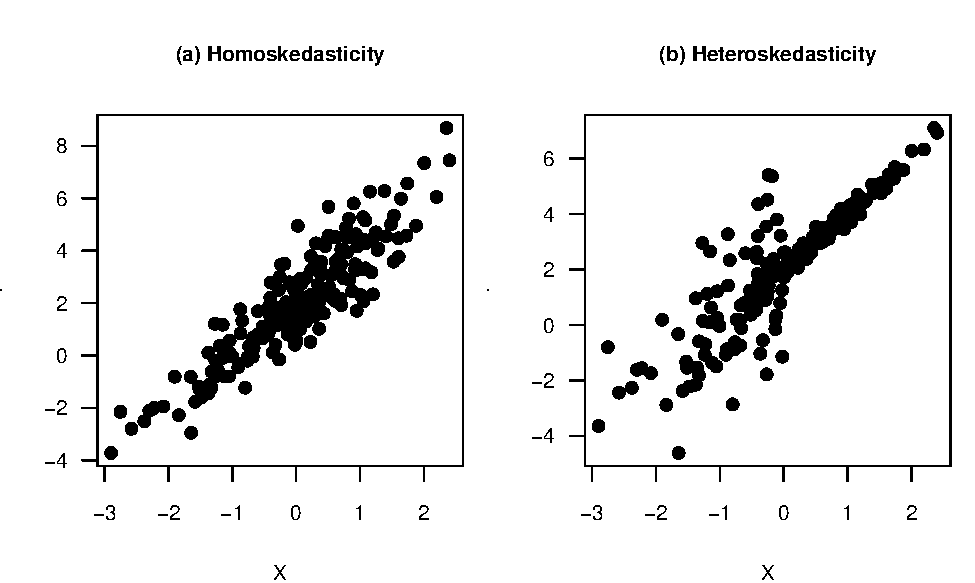
\includegraphics[width=0.9\linewidth]{AdvECTS_files/figure-latex/heteroskedasticity-1} 

}

\caption{Homoskedasticity vs heteroskedasticity.}\label{fig:heteroskedasticity}
\end{figure}

Figure \ref{fig:exmpSalarayPhDSHP} shows a situation of heteroskedasticity, based on data taken from the \href{https://forscenter.ch/projects/swiss-household-panel/}{Swiss Household Panel}. The sample is restricted to persons younger than 35 year in 2019, and that have completed at least 19 years of study. The figure shows that the dispersion of yearly income increases with age.

\begin{Shaded}
\begin{Highlighting}[]
\FunctionTok{library}\NormalTok{(AEC)}
\FunctionTok{table}\NormalTok{(shp}\SpecialCharTok{$}\NormalTok{edyear19)}
\end{Highlighting}
\end{Shaded}

\begin{verbatim}
## 
##    8    9   10   12   13   14   16   19   21 
##   70  325  350 1985  454  117  990 1263  168
\end{verbatim}

\begin{Shaded}
\begin{Highlighting}[]
\NormalTok{shp\_higherEd }\OtherTok{\textless{}{-}} \FunctionTok{subset}\NormalTok{(shp,(edyear19}\SpecialCharTok{\textgreater{}}\DecValTok{18}\NormalTok{)}\SpecialCharTok{\&}\NormalTok{age19}\SpecialCharTok{\textless{}}\DecValTok{35}\NormalTok{)}
\FunctionTok{plot}\NormalTok{(i19wyg}\SpecialCharTok{/}\DecValTok{1000}\SpecialCharTok{\textasciitilde{}}\NormalTok{age19,}\AttributeTok{data=}\NormalTok{shp\_higherEd,}\AttributeTok{pch=}\DecValTok{19}\NormalTok{,}\AttributeTok{las=}\DecValTok{1}\NormalTok{,}\AttributeTok{xlab=}\StringTok{"Age"}\NormalTok{,}\AttributeTok{ylab=}\StringTok{"Yearly work income"}\NormalTok{)}
\FunctionTok{abline}\NormalTok{(}\FunctionTok{lm}\NormalTok{(i19wyg}\SpecialCharTok{/}\DecValTok{1000}\SpecialCharTok{\textasciitilde{}}\NormalTok{age19,}\AttributeTok{data=}\NormalTok{shp\_higherEd),}\AttributeTok{col=}\StringTok{"red"}\NormalTok{,}\AttributeTok{lwd=}\DecValTok{2}\NormalTok{)}
\end{Highlighting}
\end{Shaded}

\begin{figure}
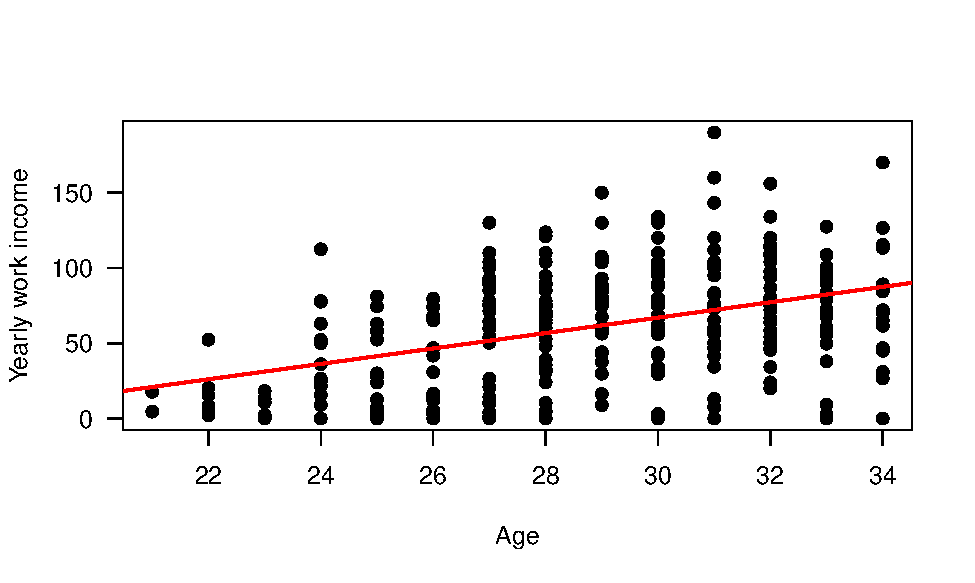
\includegraphics[width=0.95\linewidth]{AdvECTS_files/figure-latex/exmpSalarayPhDSHP-1} \caption{Income versus age. Data are from the Swiss Household Panel. The sample is restricted to persons that have completed at least 19 years of study. The figure shows that the dispersion of yearly income increases with age.}\label{fig:exmpSalarayPhDSHP}
\end{figure}

The next assumption concers the correlation of the errors across entities.

\begin{hypothesis}[Uncorrelated errors]
\protect\hypertarget{hyp:noncorrelResid}{}\label{hyp:noncorrelResid}\[
\forall i \ne j, \quad \mathbb{C}ov(\varepsilon_i,\varepsilon_j|\mathbf{X})=0.
\]
\end{hypothesis}

We will often work with covariance matrices. Proposition \ref{prp:Sigma} give the specific form of the conditional covariance of the errors when both Hpoytheses \ref{hyp:homoskedasticity} and \ref{hyp:noncorrelResid} are satisfied.

\begin{proposition}
\protect\hypertarget{prp:Sigma}{}\label{prp:Sigma}If Hpoytheses \ref{hyp:homoskedasticity} and \ref{hyp:noncorrelResid} hold, then:
\[
\mathbb{V}ar(\boldsymbol\varepsilon|\mathbf{X})= \sigma^2 Id,
\]
where \(Id\) is the \(n \times n\) identity matrix.
\end{proposition}

We will sometimes assume that errors are Gaussian --- or normal. We will then work under Hypothesis \ref{hyp:normality}:

\begin{hypothesis}[Normal distribution]
\protect\hypertarget{hyp:normality}{}\label{hyp:normality}\[
\forall i, \quad \varepsilon_i \sim \mathcal{N}(0,\sigma^2).
\]
\end{hypothesis}

\hypertarget{LSquares}{%
\section{Least square estimation}\label{LSquares}}

\hypertarget{derivation-of-the-ols-formula}{%
\subsection{Derivation of the OLS formula}\label{derivation-of-the-ols-formula}}

In this section, we will present and study the properties of the very popular estimation approach called \textbf{Ordinary Least Squares (OLS)}. As suggested by its name, the OLS estimator of \(\boldsymbol\beta\) is defined as the vector \(\mathbf{b}\) that minimizes the sum of squared residuals. (The \textbf{residuals} are the estimates of the \textbf{errors} \(\varepsilon_i\).)

For a given vector of coefficients \(\mathbf{b}=[b_1,\dots,b_K]'\), the sum of squared residuals is:
\[
f(\mathbf{b}) =\sum_{i=1}^n \left(y_i - \sum_{j=1}^K x_{i,j} b_j \right)^2 = \sum_{i=1}^n (y_i - \mathbf{x}_i' \mathbf{b})^2.
\]
Minimizing this sum amounts to minimizing:
\[
f(\mathbf{b}) = (\mathbf{y} - \mathbf{X}\mathbf{b})'(\mathbf{y} - \mathbf{X}\mathbf{b}).
\]

Since:
\[
\frac{\partial f}{\partial \mathbf{b}}(\mathbf{b}) = - 2 \mathbf{X}'\mathbf{y} + 2 \mathbf{X}'\mathbf{X}\mathbf{b},
\]
it comes that a necessary first-order condition (FOC) is:
\begin{equation}
\mathbf{X}'\mathbf{X}\mathbf{b} = \mathbf{X}'\mathbf{y}.\label{eq:OLSFOC}
\end{equation}
Under Assumption \ref{hyp:fullrank}, \(\mathbf{X}'\mathbf{X}\) is invertible. Hence:
\[
\boxed{\mathbf{b} = (\mathbf{X}'\mathbf{X})^{-1} \mathbf{X}'\mathbf{y}.}
\]
Vector \(\mathbf{b}\) minimizes the sum of squared residuals. (\(f\) is a non-negative quadratic function, it therefore admits a minimum.)

We have:
\[
\mathbf{y} = \underbrace{\mathbf{X}\mathbf{b}}_{\mbox{fitted values } (\mathbf{y})} + \underbrace{\mathbf{e}}_{\mbox{residuals}}
\]

The estimated residuals are:
\begin{equation}
\mathbf{e} = \mathbf{y} - \mathbf{X} (\mathbf{X}'\mathbf{X})^{-1} \mathbf{X}' \mathbf{y} = \mathbf{M} \mathbf{y}\label{eq:Mres}
\end{equation}
where \(\mathbf{M} := \mathbf{I} - \mathbf{X} (\mathbf{X}'\mathbf{X})^{-1} \mathbf{X}'\) is called the \textbf{residual maker} matrix.

Moreover, the fitted values \(\hat{\mathbf{y}}\) are given by:
\begin{equation}
\hat{\mathbf{y}}=\mathbf{X} (\mathbf{X}'\mathbf{X})^{-1} \mathbf{X}' \mathbf{y} = \mathbf{P} \mathbf{y},\label{eq:Proj}
\end{equation}
where \(\mathbf{P}=\mathbf{X} (\mathbf{X}'\mathbf{X})^{-1} \mathbf{X}'\) is a \textbf{projection matrix}.

These matrices \(\mathbf{M}\) and \(\mathbf{P}\) are such that:

\begin{itemize}
\tightlist
\item
  \(\mathbf{M} \mathbf{X} = \mathbf{0}\): if one regresses one of the explanatory variables on \(\mathbf{X}\), the residuals are null.
\item
  \(\mathbf{M}\mathbf{y}=\mathbf{M}\boldsymbol\varepsilon\) (because \(\mathbf{y} = \mathbf{X}\boldsymbol\beta + \boldsymbol\varepsilon\) and \(\mathbf{M} \mathbf{X} = \mathbf{0}\)).
\end{itemize}

Here are some additional properties of \(\mathbf{M}\) and \(\mathbf{P}\):

\begin{itemize}
\tightlist
\item
  \(\mathbf{M}\) is symmetric (\(\mathbf{M} = \mathbf{M}'\)) and \textbf{idempotent} (\(\mathbf{M} = \mathbf{M}^2 = \mathbf{M}^k\) for \(k>0\)).
\item
  \(\mathbf{P}\) is symmetric and idempotent.
\item
  \(\mathbf{P}\mathbf{X} = \mathbf{X}\).
\item
  \(\mathbf{P} \mathbf{M} = \mathbf{M} \mathbf{P} = 0\).
\item
  \(\mathbf{y} = \mathbf{P}\mathbf{y} + \mathbf{M}\mathbf{y}\) (decomposition of \(\mathbf{y}\) into two orthogonal parts).
\end{itemize}

It is easily checked that \(\mathbf{X}'\mathbf{e}=0\). Each column of \(\mathbf{X}\) is therefore orthogonal to \(\mathbf{e}\). In particular, if an intercept is included in the regression (\(x_{i,1} \equiv 1\), i.e., the first column of \(\mathbf{X}\) is filled with ones), the average of the residuals is null.

\begin{example}[Bivariate case]
\protect\hypertarget{exm:bivar}{}\label{exm:bivar}Consider a bivariate situation, where we regress\(y_i\) on a constant and an explanatory variable \(w_i\). We have \(K=2\), and \(\mathbf{X}\) is a \(n \times 2\) matrix whose \(i^{th}\) row is \([x_{i,1},x_{i,2}]\), with \(x_{i,1}=1\) (to account for the intercept) and with \(w_i = x_{i,2}\) (say).

We have:
\begin{eqnarray*}
\mathbf{X}'\mathbf{X} &=& 
\left[\begin{array}{cc}
n & \sum_i w_i \\
\sum_i w_i & \sum_i w_i^2
\end{array}
\right],\\
(\mathbf{X}'\mathbf{X})^{-1} &=& 
\frac{1}{n\sum_i w_i^2-(\sum_i w_i)^2}
\left[\begin{array}{cc}
\sum_i w_i^2 & -\sum_i w_i \\
-\sum_i w_i & n
\end{array}
\right],\\
(\mathbf{X}'\mathbf{X})^{-1}\mathbf{X}'\mathbf{y} &=& 
\frac{1}{n\sum_i w_i^2-(\sum_i w_i)^2}
\left[\begin{array}{c}
\sum_i w_i^2\sum_i y_i -\sum_i w_i \sum_i w_iy_i \\
-\sum_i w_i \sum_i y_i + n \sum_i w_i y_i
\end{array}
\right]\\
&=& \frac{1}{\frac{1}{n}\sum_i(w_i - \bar{w})^2}
\left[\begin{array}{c}
\frac{\bar{y}}{n}\sum_i w_i^2 -\frac{\bar{w}}{n}\sum_i w_iy_i \\
\frac{1}{n}\sum_i (w_i-\bar{w})(y_i-\bar{y})
\end{array}
\right].
\end{eqnarray*}

It can be seen that the second element of \(\mathbf{b}=(\mathbf{X}'\mathbf{X})^{-1}\mathbf{X}'\mathbf{y}\) is:
\[
b_2 = \frac{\overline{\mathbb{C}ov(W,Y)}}{\overline{\mathbb{V}ar(W)}},
\]
where \(\overline{\mathbb{C}ov(W,Y)}\) and \(\overline{\mathbb{V}ar(W)}\) are sample estimates.

Since there is a constant in the regression, we have \(b_1 = \bar{y} - b_2 \bar{w}\).
\end{example}

\hypertarget{properties-of-the-ols-estimate-small-sample}{%
\subsection{Properties of the OLS estimate (small sample)}\label{properties-of-the-ols-estimate-small-sample}}

Proposition \ref{prp:propOLS} states first properties of the OLS estimator:

\begin{proposition}[Properties of the OLS estimator]
\protect\hypertarget{prp:propOLS}{}\label{prp:propOLS}

We have:

\begin{enumerate}
\def\labelenumi{\roman{enumi}.}
\item
  Under Assumptions \ref{hyp:fullrank} and \ref{hyp:exogeneity}, the OLS estimator is linear and unbiased.
\item
  Under Hypotheses \ref{hyp:fullrank} to \ref{hyp:noncorrelResid}, the conditional covariance matrix of \(\mathbf{b}\) is: \(\mathbb{V}ar(\mathbf{b}|\mathbf{X}) = \sigma^2 (\mathbf{X}'\mathbf{X})^{-1}\).
\end{enumerate}

\end{proposition}

\begin{proof}

Under Hypothesis \ref{hyp:fullrank}, \(\mathbf{X}'\mathbf{X}\) can be inverted. We have:
\[
\mathbf{b} = (\mathbf{X}'\mathbf{X})^{-1} \mathbf{X}'\mathbf{y} = \boldsymbol\beta + (\mathbf{X}'\mathbf{X})^{-1} \mathbf{X}' \mathbf{\varepsilon}.
\]

\begin{enumerate}
\def\labelenumi{\roman{enumi}.}
\tightlist
\item
  Let us consider the expectation of the last term, i.e.~\(\mathbb{E}((\mathbf{X}'\mathbf{X})^{-1} \mathbf{X}' \mathbf{\varepsilon})\). Using the law of iterated expectations, we obtain:
  \[
  \mathbb{E}((\mathbf{X}'\mathbf{X})^{-1} \mathbf{X}' \mathbf{\varepsilon}) = \mathbb{E}(\mathbb{E}[(\mathbf{X}'\mathbf{X})^{-1} \mathbf{X}' \mathbf{\varepsilon}|\mathbf{X}]) = \mathbb{E}((\mathbf{X}'\mathbf{X})^{-1} \mathbf{X}'\mathbb{E}[\mathbf{\varepsilon}|\mathbf{X}]).
  \]
  By Hypothesis \ref{hyp:exogeneity}, we have \(\mathbb{E}[\mathbf{\varepsilon}|\mathbf{X}]=0\). Hence \(\mathbb{E}((\mathbf{X}'\mathbf{X})^{-1} \mathbf{X}' \mathbf{\varepsilon}) =0\) and result (i) follows.
\item
  \(\mathbb{V}ar(\mathbf{b}|\mathbf{X}) = (\mathbf{X}'\mathbf{X})^{-1} \mathbf{X}' \mathbb{E}(\boldsymbol\varepsilon\boldsymbol\varepsilon'|\mathbf{X}) \mathbf{X} (\mathbf{X}'\mathbf{X})^{-1}\).
  By Prop. \ref{prp:Sigma}, if \ref{hyp:homoskedasticity} and \ref{hyp:noncorrelResid} hold, then we have \(\mathbb{E}(\boldsymbol\varepsilon\boldsymbol\varepsilon'|\mathbf{X})=\mathbb{V}ar(\boldsymbol\varepsilon|\mathbf{X})=\sigma^2 Id\).
\end{enumerate}

\end{proof}

Together, Hypotheses \ref{hyp:fullrank} to \ref{hyp:noncorrelResid} form the Gauss-Markov set of assumptions. Under these assumptions, the OLS estimator feature the lowest possible variance:

\begin{theorem}[Gauss-Markov Theorem]
\protect\hypertarget{thm:GaussMarkov}{}\label{thm:GaussMarkov}Under Assumptions \ref{hyp:fullrank} to \ref{hyp:noncorrelResid}, for any vector \(w\), the minimum-variance linear unbiased estimator of \(w' \boldsymbol\beta\) is \(w' \mathbf{b}\), where \(\mathbf{b}\) is the least squares estimator. (BLUE: Best Linear Unbiased Estimator.)
\end{theorem}

\begin{proof}
Consider \(\mathbf{b}^* = C \mathbf{y}\), another linear unbiased estimator of \(\boldsymbol\beta\). Since it is unbiased, we must have \(\mathbb{E}(C\mathbf{y}|\mathbf{X}) = \mathbb{E}(C\mathbf{X}\boldsymbol\beta + C\boldsymbol\varepsilon|\mathbf{X}) = \boldsymbol\beta\). We have \(\mathbb{E}(C\boldsymbol\varepsilon|\mathbf{X})=C\mathbb{E}(\boldsymbol\varepsilon|\mathbf{X})=0\) (by \ref{hyp:exogeneity}).

Therefore \(\mathbf{b}^*\) is unbiased if \(\mathbb{E}(C\mathbf{X})\boldsymbol\beta=\boldsymbol\beta\). This has to be the case for any \(\boldsymbol\beta\), which implies that we must have \(C\mathbf{X}=\mathbf{I}\).

Let us compute \(\mathbb{V}ar(\mathbf{b^*}|\mathbf{X})\). For this, we introduce \(D = C - (\mathbf{X}'\mathbf{X})^{-1}\mathbf{X}'\), which is such that \(D\mathbf{y}=\mathbf{b}^*-\mathbf{b}\). The fact that \(C\mathbf{X}=\mathbf{I}\) implies that \(D\mathbf{X} = \mathbf{0}\).

We have \(\mathbb{V}ar(\mathbf{b^*}|\mathbf{X}) = \mathbb{V}ar(C \mathbf{y}|\mathbf{X}) =\mathbb{V}ar(C \boldsymbol\varepsilon|\mathbf{X}) = \sigma^2CC'\) (by Assumptions \ref{hyp:homoskedasticity} and \ref{hyp:noncorrelResid}, see Prop. \ref{prp:Sigma}). Using \(C=D+(\mathbf{X}'\mathbf{X})^{-1}\mathbf{X}'\) and exploiting the fact that \(D\mathbf{X} = \mathbf{0}\) leads to:
\[
\mathbb{V}ar(\mathbf{b^*}|\mathbf{X}) =\sigma^2\left[(D+(\mathbf{X}'\mathbf{X})^{-1}\mathbf{X}')(D+(\mathbf{X}'\mathbf{X})^{-1}\mathbf{X}')'\right] = \mathbb{V}ar(\mathbf{b}|\mathbf{X}) + \sigma^2 \mathbf{D}\mathbf{D}'.
\]
Therefore, we have \(\mathbb{V}ar(w'\mathbf{b^*}|\mathbf{X})=w'\mathbb{V}ar(\mathbf{b}|\mathbf{X})w + \sigma^2 w'\mathbf{D}\mathbf{D}'w\ge w'\mathbb{V}ar(\mathbf{b}|\mathbf{X})w=\mathbb{V}ar(w'\mathbf{b}|\mathbf{X})\).
\end{proof}

The Frish-Waugh theorem (Theorem \ref{thm:FW}) reveals the relationship between the OLS estimator and the notion of partial correlation coefficient. Consider the linear least square regression of \(\mathbf{y}\) on \(\mathbf{X}\). We introduce the notations:

\begin{itemize}
\tightlist
\item
  \(\mathbf{b}^{\mathbf{y}/\mathbf{X}}\): OLS estimates of \(\boldsymbol\beta\),
\item
  \(\mathbf{M}^{\mathbf{X}}\): residual-maker matrix of any regression on \(\mathbf{X}\),
\item
  \(\mathbf{P}^{\mathbf{X}}\): projection matrix of any regression on \(\mathbf{X}\).
\end{itemize}

Let us split the set of explanatory variables into two: \(\mathbf{X} = [\mathbf{X}_1,\mathbf{X}_2]\). With obvious notations: \(\mathbf{b}^{\mathbf{y}/\mathbf{X}}=[\mathbf{b}_1',\mathbf{b}_2']'\).

\begin{theorem}[Frisch-Waugh Theorem]
\protect\hypertarget{thm:FW}{}\label{thm:FW}We have:
\[
\mathbf{b}_2 = \mathbf{b}^{\mathbf{M^{\mathbf{X}_1}y}/\mathbf{M^{\mathbf{X}_1}\mathbf{X}_2}}.
\]
\end{theorem}

\begin{proof}
The minimization of the least squares leads to (these are first-order conditions, see Eq. \eqref{eq:OLSFOC}):
\[
\left[ \begin{array}{cc} \mathbf{X}_1'\mathbf{X}_1 & \mathbf{X}_1'\mathbf{X}_2 \\ \mathbf{X}_2'\mathbf{X}_1 & \mathbf{X}_2'\mathbf{X}_2\end{array}\right]
\left[ \begin{array}{c} \mathbf{b}_1 \\ \mathbf{b}_2\end{array}\right] =
\left[ \begin{array}{c} \mathbf{X}_1' \mathbf{y} \\ \mathbf{X}_2' \mathbf{y} \end{array}\right].
\]
Use the first-row block of equations to solve for \(\mathbf{b}_1\) first; it comes as a function of \(\mathbf{b}_2\). Then use the second set of equations to solve for \(\mathbf{b}_2\), which leads to:
\[
\mathbf{b}_2 = [\mathbf{X}_2'\mathbf{X}_2 - \mathbf{X}_2'\mathbf{X}_1(\mathbf{X}_1'\mathbf{X}_1)\mathbf{X}_1'\mathbf{X}_2]^{-1}\mathbf{X}_2'(Id - \mathbf{X}_1(\mathbf{X}_1'\mathbf{X}_1)\mathbf{X}_1')\mathbf{y}=[\mathbf{X}_2' \mathbf{M}^{\mathbf{X}_1}\mathbf{X}_2]^{-1}\mathbf{X}_2'\mathbf{M}^{\mathbf{X}_1}\mathbf{y}.
\]
Using the fact that \(\mathbf{M}^{\mathbf{X}_1}\) is idempotent and symmetric leads to the result.
\end{proof}

This suggests a second way of estimating \(\mathbf{b}_2\):

\begin{enumerate}
\def\labelenumi{\arabic{enumi}.}
\tightlist
\item
  Regress \(Y\) on \(X_1\), regress \(X_2\) on \(X_1\).
\item
  Regress the residuals associated with the former regression on the ones associated withe the latter regressions.
\end{enumerate}

This is illustrated by the following code, where we run different regressions involving the number of Google searches for ``parapluie'' (\emph{umbrella} in French) In the broad specification, we regress it on French precipitations and month dummies. Next, we deseasonalize both the dependent variable and the precipitations by regressing them on the month dummies. As stated by Theorem \ref{thm:FW}, regressing deseasonalized Google searches on deseasonalized precipitations give the same coefficient as in the baseline regression.

\begin{Shaded}
\begin{Highlighting}[]
\FunctionTok{library}\NormalTok{(AEC)}
\NormalTok{dummies }\OtherTok{\textless{}{-}} \FunctionTok{as.matrix}\NormalTok{(parapluie[,}\DecValTok{4}\SpecialCharTok{:}\DecValTok{14}\NormalTok{])}
\NormalTok{eq\_all }\OtherTok{\textless{}{-}} \FunctionTok{lm}\NormalTok{(parapluie}\SpecialCharTok{\textasciitilde{}}\NormalTok{precip}\SpecialCharTok{+}\NormalTok{dummies,}\AttributeTok{data=}\NormalTok{parapluie)}
\NormalTok{deseas\_parapluie }\OtherTok{\textless{}{-}} \FunctionTok{lm}\NormalTok{(parapluie}\SpecialCharTok{\textasciitilde{}}\NormalTok{dummies,}\AttributeTok{data=}\NormalTok{parapluie)}\SpecialCharTok{$}\NormalTok{residuals}
\NormalTok{deseas\_precip    }\OtherTok{\textless{}{-}} \FunctionTok{lm}\NormalTok{(precip}\SpecialCharTok{\textasciitilde{}}\NormalTok{dummies,}\AttributeTok{data=}\NormalTok{parapluie)}\SpecialCharTok{$}\NormalTok{residuals}
\NormalTok{eq\_frac }\OtherTok{\textless{}{-}} \FunctionTok{lm}\NormalTok{(deseas\_parapluie}\SpecialCharTok{\textasciitilde{}}\NormalTok{deseas\_precip)}
\FunctionTok{rbind}\NormalTok{(eq\_all}\SpecialCharTok{$}\NormalTok{coefficients,}
      \FunctionTok{c}\NormalTok{(eq\_frac}\SpecialCharTok{$}\NormalTok{coefficients,}\FunctionTok{rep}\NormalTok{(}\ConstantTok{NaN}\NormalTok{,}\DecValTok{11}\NormalTok{)))}
\end{Highlighting}
\end{Shaded}

\begin{verbatim}
##        (Intercept)    precip  dummies1  dummies2  dummies3  dummies4  dummies5
## [1,] -2.953448e+00 0.1300055 -8.599068 -13.32904 -7.982958 -3.392353 -3.703816
## [2,] -1.038345e-15 0.1300055       NaN       NaN       NaN       NaN       NaN
##       dummies6  dummies7  dummies8 dummies9 dummies10 dummies11
## [1,] -3.360641 -7.315881 -7.717277  -4.6492 -5.109199   1.98077
## [2,]       NaN       NaN       NaN      NaN       NaN       NaN
\end{verbatim}

When \(b_2\) is scalar (and then \(\mathbf{X}_2\) is of dimension \(n \times 1\)), Theorem \ref{thm:FW} gives the expression of the \textbf{partial regression coefficient} \(b_2\):
\[
b_2 = \frac{\mathbf{X}_2'M^{\mathbf{X}_1}\mathbf{y}}{\mathbf{X}_2'M^{\mathbf{X}_1}\mathbf{X}_2}.
\]

\hypertarget{goodness-of-fit}{%
\subsection{Goodness of fit}\label{goodness-of-fit}}

Define the total variation in \(y\) as the sum of squared deviations:
\[
TSS = \sum_{i=1}^{n} (y_i - \bar{y})^2.
\]
We have:
\[
\mathbf{y} = \mathbf{X}\mathbf{b} + \mathbf{e} = \hat{\mathbf{y}} + \mathbf{e}
\]
In the following, we assume that the regression includes a constant (i.e.~for all \(i\), \(x_{i,1}=1\)). Denote by \(\mathbf{M}^0\) the matrix that transforms observations into deviations from sample means. Using that \(\mathbf{M}^0 \mathbf{e} = \mathbf{e}\) and that \(\mathbf{X}' \mathbf{e}=0\), we have:
\begin{eqnarray*}
\underbrace{\mathbf{y}'\mathbf{M}^0\mathbf{y}}_{\mbox{Total sum of sq.}} &=& (\mathbf{X}\mathbf{b} + \mathbf{e})' \mathbf{M}^0 (\mathbf{X}\mathbf{b} + \mathbf{e})\\
&=& \underbrace{\mathbf{b}' \mathbf{X}' \mathbf{M}^0 \mathbf{X}\mathbf{b}}_{\mbox{"Explained" sum of sq.}} + \underbrace{\mathbf{e}'\mathbf{e}}_{\mbox{Sum of sq. residuals}}\\
TSS &=& Expl.SS + SSR.
\end{eqnarray*}

We can now define the coefficient of determination:
\begin{equation}
\boxed{\mbox{Coefficient of determination} = \frac{Expl.SS}{TSS} = 1 - \frac{SSR}{TSS} = 1 - \frac{\mathbf{e}'\mathbf{e}}{\mathbf{y}'\mathbf{M}^0\mathbf{y}}.}\label{eq:RR2}
\end{equation}

It can be shown \citep[Section 3.5]{Greene2003Econometric} that:
\[
\mbox{Coefficient of determination} = \frac{[\sum_{i=1}^n(y_i - \bar{y})(\hat{y_i} - \bar{y})]^2}{\sum_{i=1}^n(y_i - \bar{y})^2 \sum_{i=1}^n(\hat{y_i} - \bar{y})^2}.
\]
That is, the \(R^2\) is the sample squared correlation between \(y\) and the (regression-implied) \(y\)'s predictions.

The hgher the \(R^2\), the higher the goodness of fit of a model. One however has to be cautious with \(R^2\). Indeed, it is easy to increase it: it suffices to add explanatory variables. As stated by Proposition \ref{prp:chgeInR2}, adding an explanatory variable (even if it does not truly relate to the dependent variable) results in an increase in the \(R^2\). In the limit, taking any set of \(n\) non-linearly-dependent explanatory variables (i.e., variables satisfying Hypothesis \ref{hyp:fullrank}) results in a \(R^2\) equal to one.

\begin{proposition}[Change in SSR when a variable is added]
\protect\hypertarget{prp:chgeR2}{}\label{prp:chgeR2}We have:
\begin{equation}
\mathbf{u}'\mathbf{u} = \mathbf{e}'\mathbf{e} - c^2(\mathbf{z^*}'\mathbf{z^*}) \qquad (\le \mathbf{e}'\mathbf{e}) \label{eq:uu}
\end{equation}
where (i) \(\mathbf{u}\) and \(\mathbf{e}\) are the residuals in the regressions of \(\mathbf{y}\) on \([\mathbf{X},\mathbf{z}]\) and of \(\mathbf{y}\) on \(\mathbf{X}\), respectively, (ii) \(c\) is the regression coefficient on \(\mathbf{z}\) in the former regression and where \(\mathbf{z}^*\) are the residuals in the regression of \(\mathbf{z}\) on \(\mathbf{X}\).
\end{proposition}

\begin{proof}
The OLS estimates \([\mathbf{d}',\mathbf{c}]'\) in the regression of \(\mathbf{y}\) on \([\mathbf{X},\mathbf{z}]\) satisfies (first-order cond., Eq. \eqref{eq:OLSFOC})
\[
\left[ \begin{array}{cc} \mathbf{X}'\mathbf{X} & \mathbf{X}'\mathbf{z} \\ \mathbf{z}'\mathbf{X} & \mathbf{z}'\mathbf{z}\end{array}\right]
\left[ \begin{array}{c} \mathbf{d} \\ \mathbf{c}\end{array}\right] =
\left[ \begin{array}{c} \mathbf{X}' \mathbf{y} \\ \mathbf{z}' \mathbf{y} \end{array}\right].
\]
Hence, in particular \(\mathbf{d} = \mathbf{b} - (\mathbf{X}'\mathbf{X})^{-1}\mathbf{X}'\mathbf{z}\mathbf{c}\), where \(\mathbf{b}\) is the OLS of \(\mathbf{y}\) on \(\mathbf{X}\). Substituting in \(\mathbf{u} = \mathbf{y} - \mathbf{X}\mathbf{d} - \mathbf{z}c\), we get \(\mathbf{u} = \mathbf{e} - \mathbf{z}^*c\). We therefore have:
\begin{equation}
\mathbf{u}'\mathbf{u} = (\mathbf{e} - \mathbf{z}^*c)(\mathbf{e} - \mathbf{z}^*c)= \mathbf{e}'\mathbf{e} + c^2(\mathbf{z^*}'\mathbf{z^*}) - 2 c\mathbf{z^*}'\mathbf{e}.\label{eq:uuu}
\end{equation}
Now \(\mathbf{z^*}'\mathbf{e} = \mathbf{z^*}'(\mathbf{y} - \mathbf{X}\mathbf{b}) = \mathbf{z^*}'\mathbf{y}\) because \(\mathbf{z}^*\) are the residuals in an OLS regression on \(\mathbf{X}\). Since \(c = (\mathbf{z^*}'\mathbf{z^*})^{-1}\mathbf{z^*}'\mathbf{y^*}\) (by an application of Theorem \ref{thm:FW}), we have \((\mathbf{z^*}'\mathbf{z^*})c = \mathbf{z^*}'\mathbf{y^*}\) and, therefore, \(\mathbf{z^*}'\mathbf{e} = (\mathbf{z^*}'\mathbf{z^*})c\). Inserting this in Eq. \eqref{eq:uuu} leads to the results.
\end{proof}

\begin{proposition}[Change in the coefficient of determination when a variable is added]
\protect\hypertarget{prp:chgeInR2}{}\label{prp:chgeInR2}Denoting by \(R_W^2\) the coefficient of determination in the regression of \(\mathbf{y}\) on some variable \(\mathbf{W}\), we have:
\[
R_{\mathbf{X},\mathbf{z}}^2 = R_{\mathbf{X}}^2 + (1-R_{\mathbf{X}}^2)(r_{yz}^\mathbf{X})^2,
\]
where \(r_{yz}^\mathbf{X}\) is the coefficient of partial correlation (see Definition \ref{def:partialcorrel}).
\end{proposition}

\begin{proof}
Let's use the same notations as in Prop. @ref\{prp:chgeR2\}. Theorem \ref{thm:FW} implies that \(c = (\mathbf{z^*}'\mathbf{z^*})^{-1}\mathbf{z^*}'\mathbf{y^*}\). Using this in Eq. \eqref{eq:uu} gives \(\mathbf{u}'\mathbf{u} = \mathbf{e}'\mathbf{e} - (\mathbf{z^*}'\mathbf{y^*})^2/(\mathbf{z^*}'\mathbf{z^*})\). Using the definition of the partial correlation (Eq. \eqref{eq:pc}), we get \(\mathbf{u}'\mathbf{u} = \mathbf{e}'\mathbf{e}\left(1 - (r_{yz}^\mathbf{X})^2\right)\). The results is obtained by dividing both sides of the previous equation by \(\mathbf{y}'\mathbf{M}_0\mathbf{y}\).
\end{proof}

Figure \ref{fig:R2issue}, below, illustrates the fact that one can obtain an \(R^2\) of one by regressing a sample of length \(n\) on any set of \(n\) linearly-independent variables.

\begin{Shaded}
\begin{Highlighting}[]
\NormalTok{n }\OtherTok{\textless{}{-}} \DecValTok{30}\NormalTok{;Y }\OtherTok{\textless{}{-}} \FunctionTok{rnorm}\NormalTok{(n);X }\OtherTok{\textless{}{-}} \FunctionTok{matrix}\NormalTok{(}\FunctionTok{rnorm}\NormalTok{(n}\SpecialCharTok{\^{}}\DecValTok{2}\NormalTok{),n,n)}
\NormalTok{all\_R2 }\OtherTok{\textless{}{-}} \ConstantTok{NULL}\NormalTok{;all\_adjR2 }\OtherTok{\textless{}{-}} \ConstantTok{NULL}
\ControlFlowTok{for}\NormalTok{(j }\ControlFlowTok{in} \DecValTok{0}\SpecialCharTok{:}\NormalTok{(n}\DecValTok{{-}1}\NormalTok{))\{}
  \ControlFlowTok{if}\NormalTok{(j}\SpecialCharTok{==}\DecValTok{0}\NormalTok{)\{eq }\OtherTok{\textless{}{-}} \FunctionTok{lm}\NormalTok{(Y}\SpecialCharTok{\textasciitilde{}}\DecValTok{1}\NormalTok{)}
\NormalTok{  \}}\ControlFlowTok{else}\NormalTok{\{eq }\OtherTok{\textless{}{-}} \FunctionTok{lm}\NormalTok{(Y}\SpecialCharTok{\textasciitilde{}}\NormalTok{X[,}\DecValTok{1}\SpecialCharTok{:}\NormalTok{j])\}}
\NormalTok{  all\_R2 }\OtherTok{\textless{}{-}} \FunctionTok{c}\NormalTok{(all\_R2,}\FunctionTok{summary}\NormalTok{(eq)}\SpecialCharTok{$}\NormalTok{r.squared)}
\NormalTok{  all\_adjR2 }\OtherTok{\textless{}{-}} \FunctionTok{c}\NormalTok{(all\_adjR2,}\FunctionTok{summary}\NormalTok{(eq)}\SpecialCharTok{$}\NormalTok{adj.r.squared)}
\NormalTok{\}}
\FunctionTok{plot}\NormalTok{(all\_R2,}\AttributeTok{pch=}\DecValTok{19}\NormalTok{,}\AttributeTok{ylim=}\FunctionTok{c}\NormalTok{(}\FunctionTok{min}\NormalTok{(all\_adjR2,}\AttributeTok{na.rm =} \ConstantTok{TRUE}\NormalTok{),}\DecValTok{1}\NormalTok{),}\AttributeTok{xlab=}\StringTok{"number of regressors"}\NormalTok{,}\AttributeTok{ylab=}\StringTok{"R2"}\NormalTok{)}
\FunctionTok{points}\NormalTok{(all\_adjR2,}\AttributeTok{pch=}\DecValTok{3}\NormalTok{);}\FunctionTok{abline}\NormalTok{(}\AttributeTok{h=}\DecValTok{0}\NormalTok{,}\AttributeTok{col=}\StringTok{"light grey"}\NormalTok{,}\AttributeTok{lwd=}\DecValTok{2}\NormalTok{)}
\FunctionTok{legend}\NormalTok{(}\StringTok{"topleft"}\NormalTok{,}\FunctionTok{c}\NormalTok{(}\StringTok{"R2"}\NormalTok{,}\StringTok{"Adjusted R2"}\NormalTok{),}
       \AttributeTok{lty=}\ConstantTok{NaN}\NormalTok{,}\AttributeTok{col=}\FunctionTok{c}\NormalTok{(}\StringTok{"black"}\NormalTok{),}\AttributeTok{pch=}\FunctionTok{c}\NormalTok{(}\DecValTok{19}\NormalTok{,}\DecValTok{3}\NormalTok{),}\AttributeTok{lwd=}\DecValTok{2}\NormalTok{)}
\end{Highlighting}
\end{Shaded}

\begin{figure}

{\centering 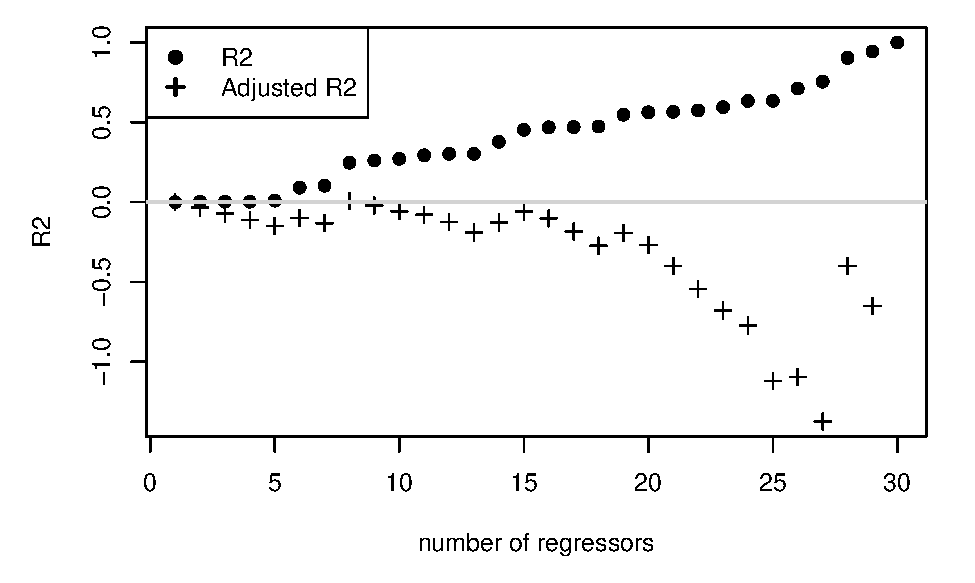
\includegraphics[width=0.9\linewidth]{AdvECTS_files/figure-latex/R2issue-1} 

}

\caption{This figure illustrates the monotonous increase in the $R^2$ as a function of the number of explanatory variables. In the true model, there is no explanatory variables, i.e., $y_i = \varepsilon_i$. We then take (independent) regressors and regress $y$ on the latter, progresively increasing the set of regressors.}\label{fig:R2issue}
\end{figure}

In order to address the risk of adding irrelevant explanatory variables, measures of \textbf{adjusted \(R^2\)} have been proposed. Compared to the standard \(R^2\), these measures add penalties that depend on the number of covariates employed in the regression. A common adjusted \(R^2\) measure, denoted by \(\bar{R}^2\), is the following:
\begin{equation*}
\boxed{\bar{R}^2 = 1 - \frac{\mathbf{e}'\mathbf{e}/(n-K)}{\mathbf{y}'\mathbf{M}^0\mathbf{y}/(n-1)} = 1 - \frac{n-1}{n-K}(1-R^2).}
\end{equation*}

\hypertarget{inference-and-confidence-intervals-in-small-sample}{%
\subsection{Inference and confidence intervals (in small sample)}\label{inference-and-confidence-intervals-in-small-sample}}

Under the normality assumption (Assumption \ref{hyp:normality}), we know the distribution of \(\mathbf{b}\) (conditional on \(\mathbf{X}\)). Indeed, \((\mathbf{b}|\mathbf{X}) \equiv (\mathbf{X}'\mathbf{X})^{-1} \mathbf{X}'\mathbf{y}\) is multivariate Gaussian:
\begin{equation}
\mathbf{b}|\mathbf{X} \sim \mathcal{N}(\beta,\sigma^2(\mathbf{X}'\mathbf{X})^{-1}).\label{eq:distriBcondi}
\end{equation}

Eq. \eqref{eq:distriBcondi} can be used to conduct inference and tests. However, in practice, we do not know \(\sigma^2\) (which is a population parameter). The following proposition gives an unbiased estimate of \(\sigma^2\).

\begin{proposition}
\protect\hypertarget{prp:expects2}{}\label{prp:expects2}Under \ref{hyp:fullrank} to \ref{hyp:noncorrelResid}, an unbiased estimate of \(\sigma^2\) is given by:
\begin{equation}
s^2 = \frac{\mathbf{e}'\mathbf{e}}{n-K}.\label{eq:s2}
\end{equation}
(It is sometimes denoted by \(\sigma^2_{OLS}\).)
\end{proposition}

\begin{proof}
\(\mathbb{E}(\mathbf{e}'\mathbf{e}|\mathbf{X})=\mathbb{E}(\boldsymbol{\varepsilon}'\mathbf{M}\boldsymbol{\varepsilon}|\mathbf{X})=\mathbb{E}(\mbox{Tr}(\boldsymbol{\varepsilon}'\mathbf{M}\boldsymbol{\varepsilon})|\mathbf{X})) =\mbox{Tr}(\mathbf{M}\mathbb{E}(\boldsymbol{\varepsilon}\boldsymbol{\varepsilon}'|\mathbf{X}))=\sigma^2 \mbox{Tr}(\mathbf{M})\). (Note that we have \(\mathbb{E}(\boldsymbol{\varepsilon}\boldsymbol{\varepsilon}'|\mathbf{X})=\sigma^2Id\) by Assumptions \ref{hyp:homoskedasticity} and \ref{hyp:noncorrelResid}, see Prop. \ref{prp:Sigma}.) Finally:
\begin{eqnarray*}
\mbox{Tr}(\mathbf{M})&=&n-\mbox{Tr}(\mathbf{X}(\mathbf{X}'\mathbf{X})^{-1}\mathbf{X}')\\
&=&n-\mbox{Tr}((\mathbf{X}'\mathbf{X})^{-1}\mathbf{X}'\mathbf{X})=n-\mbox{Tr}(Id_{K \times K}),
\end{eqnarray*}
which leads to the result.
\end{proof}

Two results will prove important to produce inference:

\begin{enumerate}
\def\labelenumi{\roman{enumi}.}
\tightlist
\item
  We know the distribution of \(s^2\) (Prop. \ref{prp:s2distri}).
\item
  \(s^2\) and \(\mathbf{b}\) are independent random variables (Prop. \ref{prp:indeps2b}).
\end{enumerate}

\begin{proposition}
\protect\hypertarget{prp:s2distri}{}\label{prp:s2distri}Under \ref{hyp:fullrank} to \ref{hyp:normality}, we have: \(\dfrac{s^2}{\sigma^2} | \mathbf{X} \sim \chi^2(n-K)/(n-K)\).
\end{proposition}

\begin{proof}
We have \(\mathbf{e}'\mathbf{e}=\boldsymbol\varepsilon'\mathbf{M}\boldsymbol\varepsilon\). \(\mathbf{M}\) is an idempotent symmetric matrix. Therefore it can be decomposed as \(PDP'\) where \(D\) is a diagonal matrix and \(P\) is an orthogonal matrix. As a result \(\mathbf{e}'\mathbf{e} = (P'\boldsymbol\varepsilon)'D(P'\boldsymbol\varepsilon)\), i.e.~\(\mathbf{e}'\mathbf{e}\) is a weighted sum of independent squared Gaussian variables (the entries of \(P'\boldsymbol\varepsilon\) are independent because they are Gaussian ---under \ref{hyp:normality}--- and uncorrelated). The variance of each of these i.i.d. Gaussian variable is \(\sigma^2\). Because \(\mathbf{M}\) is an idempotent symmetric matrix, its eigenvalues are either 0 or 1, and its rank equals its trace (see Propositions \ref{prp:rootsidempotent} and \ref{prp:chi2idempotent}). Further, its trace is equal to \(n-K\) (see proof of Eq. \eqref{eq:s2}). Therefore \(D\) has \(n-K\) entries equal to 1 and \(K\) equal to 0. Hence, \(\mathbf{e}'\mathbf{e} = (P'\boldsymbol\varepsilon)'D(P'\boldsymbol\varepsilon)\) is a sum of \(n-K\) squared independent Gaussian variables of variance \(\sigma^2\). Therefore \(\frac{\mathbf{e}'\mathbf{e}}{\sigma^2} = (n-K)\frac{s^2}{\sigma^2}\) is a sum of \(n-k\) squared i.i.d. standard normal variables.
\end{proof}

\begin{proposition}
\protect\hypertarget{prp:indeps2b}{}\label{prp:indeps2b}Under Hypotheses \ref{hyp:fullrank} to \ref{hyp:normality}, \(\mathbf{b}\) and \(s^2\) are independent.
\end{proposition}

\begin{proof}
We have \(\mathbf{b}=\boldsymbol\beta + [\mathbf{X}'{\mathbf{X}}]^{-1}\mathbf{X}\boldsymbol\varepsilon\) and \(s^2 = \boldsymbol\varepsilon' \mathbf{M} \boldsymbol\varepsilon/(n-K)\). Hence \(\mathbf{b}\) is an affine combination of \(\boldsymbol\varepsilon\) and \(s^2\) is a quadratic combination of the same Gaussian shocks. One can write \(s^2\) as \(s^2 = (\mathbf{M}\boldsymbol\varepsilon)' \mathbf{M} \boldsymbol\varepsilon/(n-K)\) and \(\mathbf{b}\) as \(\boldsymbol\beta + \mathbf{T}\boldsymbol\varepsilon\). Since \(\mathbf{T}\mathbf{M}=0\), \(\mathbf{T}\boldsymbol\varepsilon\) and \(\mathbf{M}\boldsymbol\varepsilon\) are independent (because two uncorrelated Gaussian variables are independent), therefore \(\mathbf{b}\) and \(s^2\), which are functions of two sets of independent variables, are independent.
\end{proof}

Consistently with Eq. \eqref{eq:distriBcondi}, under Hypotheses \ref{hyp:fullrank} to \ref{hyp:normality}, the \(k^{th}\) entry of \(\mathbf{b}\) satisfies:
\[
b_k | \mathbf{X} \sim \mathcal{N}(\beta_k,\sigma^2 v_k),
\]
where \(v_k\) is the k\(^{th}\) component of the diagonal of \((\mathbf{X}'\mathbf{X})^{-1}\).

Moreover, we have (Prop. \ref{prp:s2distri}):
\[
\frac{(n-K)s^2}{\sigma^2} | \mathbf{X} \sim \chi ^2 (n-K).
\]

As a result (using Propositions \ref{prp:s2distri} and \ref{prp:indeps2b}), we have:
\begin{equation}
\boxed{t_k = \frac{\frac{b_k - \beta_k}{\sqrt{\sigma^2 v_k}}}{\sqrt{\frac{(n-K)s^2}{\sigma^2(n-K)}}} = \frac{b_k - \beta_k}{\sqrt{s^2v_k}} \sim t(n-K),}\label{eq:resultstudentt}
\end{equation}
where \(t(n-K)\) denotes a \(t\) distribution with \(n-K\) degrees of freedom.\footnote{We have \(\frac{b_k - \beta_k}{\sqrt{\sigma^2 v_k}} | \mathbf{X} \sim \mathcal{N}(0,1)\) and \(\frac{(n-K)s^2}{\sigma^2} | \mathbf{X} \sim \chi ^2 (n-K)\). These two distributions do not depend on \(\mathbf{X}\) \(\Rightarrow\) the \emph{marginal distribution} of \(t_k\) is also \(t\).}

Note that \(s^2 v_k\) is not exactly the conditional variance of \(b_k\): The variance of \(b_k\) conditional on \(\mathbf{X}\) is \(\sigma^2 v_k\). However \(s^2 v_k\) is an unbiased estimate of \(\sigma^2 v_k\) (by Prop. \ref{prp:expects2}).

The previous result (Eq. \eqref{eq:resultstudentt}) can be extended to any linear combinations of elements of \(\mathbf{b}\) (Eq. \eqref{eq:resultstudentt} is for its \(k^{th}\) component only).

Let us consider \(\boldsymbol\alpha'\mathbf{b}\), the OLS estimate of \(\boldsymbol\alpha'\boldsymbol\beta\). From Eq. \eqref{eq:distriBcondi}, we have:
\[
\boldsymbol\alpha'\mathbf{b} | \mathbf{X} \sim \mathcal{N}(\boldsymbol\alpha'\boldsymbol\beta,\sigma^2 \boldsymbol\alpha'(\mathbf{X}'\mathbf{X})^{-1}\boldsymbol\alpha).
\]
Therefore:
\[
\frac{\boldsymbol\alpha'\mathbf{b} - \boldsymbol\alpha'\boldsymbol\beta}{\sqrt{\sigma^2 \boldsymbol\alpha'(\mathbf{X}'\mathbf{X})^{-1}\boldsymbol\alpha}} | \mathbf{X} \sim \mathcal{N}(0,1).
\]
Using the same approach as the one used to derive Eq. \eqref{eq:resultstudentt}, one can show that Props. \ref{prp:s2distri} and \ref{prp:indeps2b} also imply that:
\begin{equation}
\boxed{\frac{\boldsymbol\alpha'\mathbf{b} - \boldsymbol\alpha'\boldsymbol\beta}{\sqrt{s^2\boldsymbol\alpha'(\mathbf{X}'\mathbf{X})^{-1}\boldsymbol\alpha}} \sim t(n-K).}\label{eq:resultstudentt2}
\end{equation}

\begin{figure}
\centering
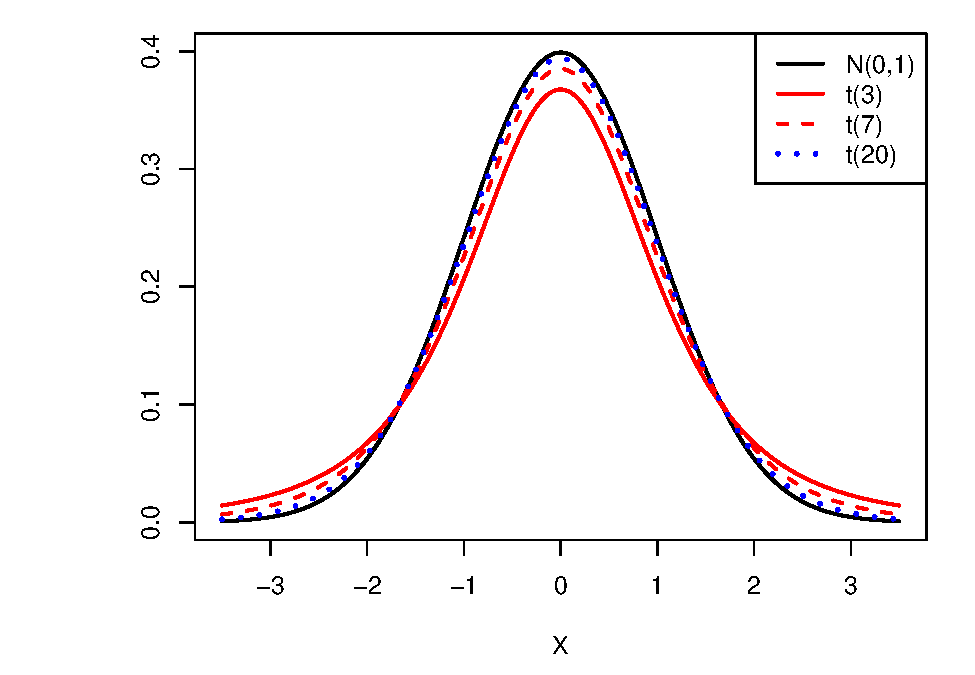
\includegraphics{AdvECTS_files/figure-latex/chartStudent-1.pdf}
\caption{\label{fig:chartStudent}The higher the degree of freedom, the closer the distribution of \(t(\nu)\) gets to the normal distribution. (Convergence in distribution.)}
\end{figure}

What precedes is widely exploited for statistical inference in the context of linear regressions. Indeed, Eq. \eqref{eq:resultstudentt} gives a sense of the distances between \(b_k\) and \(\beta_k\) that can be deemed as ``likely''. For instance, it implies that, if \(\sqrt{v_k s^2}\) is equal to 1 (say), then the probability to obtain \(b_k\) smaller than \(\beta_k-\) 4.587 \(\times \sqrt{v_k s^2}\) or larger than \(\beta_k+\) 4.587 \(\times \sqrt{v_k s^2}\) is equal to 0.1\% when \(n-K=10\).

That means for instance that, under the assumption that \(\beta_k=0\), it would be extremely unlikely to have obtained \(b_k/\sqrt{v_k s^2}\) smaller than 4.587 or larger than 4.587. More generally, this shows that the \textbf{t-statistic}, i.e., the ratio \(b_k/\sqrt{v_k s^2}\), is the test statistic associated with the null hypothesis:
\[
H_0: \beta_k=0.
\]
Under the null hypothesis, the test statistic follows a Student-t distribution with \(n-K\) degrees of freedom. The \textbf{t-statistic} is therefore of particular importance, and, as a result, it is routinely reported in regression outputs. This is illustrated below, in a regression that aims at determining covariates of households' income. This example makes use of data from the \href{https://forscenter.ch/projects/swiss-household-panel/}{Swiss Household Panel (SHP)}. \texttt{edyear19} is the number of years of education and \texttt{age19} is the age of the respondent, as of 2019.

\begin{Shaded}
\begin{Highlighting}[]
\FunctionTok{library}\NormalTok{(AEC)}
\FunctionTok{library}\NormalTok{(sandwich)}
\NormalTok{shp}\SpecialCharTok{$}\NormalTok{income }\OtherTok{\textless{}{-}}\NormalTok{ shp}\SpecialCharTok{$}\NormalTok{i19ptotn}\SpecialCharTok{/}\DecValTok{1000}
\NormalTok{shp}\SpecialCharTok{$}\NormalTok{female }\OtherTok{\textless{}{-}} \DecValTok{1}\SpecialCharTok{*}\NormalTok{(shp}\SpecialCharTok{$}\NormalTok{sex19}\SpecialCharTok{==}\DecValTok{2}\NormalTok{)}
\NormalTok{eq }\OtherTok{\textless{}{-}} \FunctionTok{lm}\NormalTok{(income }\SpecialCharTok{\textasciitilde{}}\NormalTok{ edyear19 }\SpecialCharTok{+}\NormalTok{ age19 }\SpecialCharTok{+} \FunctionTok{I}\NormalTok{(age19}\SpecialCharTok{\^{}}\DecValTok{2}\NormalTok{) }\SpecialCharTok{+}\NormalTok{ female,}\AttributeTok{data=}\NormalTok{shp)}
\end{Highlighting}
\end{Shaded}

The last two columns give the \textbf{t-statistic} and p-values associated with the t-test, whose \textbf{critical region} for the test of size \(\alpha\) is:
\[
\left]-\infty,-\Phi^{-1}_{t(n-K)}\left(1-\frac{\alpha}{2}\right)\right] \cup \left[\Phi^{-1}_{t(n-K)}\left(1-\frac{\alpha}{2}\right),+\infty\right[.
\]
We recall that the \textbf{p-value} is defined as the probability that \(|Z| > |t|\), where \(t\) is the (computed) t statistics and where \(Z \sim t(n-K)\). That is, the p-value is given by \(2(1 - \Phi_{t(n-K)}(|t_k|))\). See \href{https://jrenne.shinyapps.io/tests/}{this webpage} for details regarding the link between critical regions, p-value, and test outcomes.

Now, suppose we want to compute a (symmetrical) \textbf{confidence interval} \([I_{d,1-\alpha},I_{u,1-\alpha}]\) that is such that \(\mathbb{P}(\beta_k \in [I_{d,1-\alpha},I_{u,1-\alpha}])=1-\alpha\). In particular, we want to have: \(\mathbb{P}(\beta_k < I_{d,1-\alpha})=\frac{\alpha}{2}\).

For this purpose, we make use of Eq. \eqref{eq:resultstudentt}, i.e., \(t_k = \frac{b_k - \beta_k}{\sqrt{s^2v_k}} \sim t(n-K)\). We have:
\begin{eqnarray*}
\mathbb{P}(\beta_k < I_{d,1-\alpha})=\frac{\alpha}{2} &\Leftrightarrow& \\
\mathbb{P}\left(\frac{b_k - \beta_k}{\sqrt{s^2v_k}} > \frac{b_k - I_{d,1-\alpha}}{\sqrt{s^2v_k}}\right)=\frac{\alpha}{2} &\Leftrightarrow& \mathbb{P}\left(t_k > \frac{b_k - I_{d,1-\alpha}}{\sqrt{s^2v_k}}\right)=\frac{\alpha}{2} \Leftrightarrow\\
1 - \mathbb{P}\left(t_k \le \frac{b_k - I_{d,1-\alpha}}{\sqrt{s^2v_k}}\right)=\frac{\alpha}{2} &\Leftrightarrow& \frac{b_k - I_{d,1-\alpha}}{\sqrt{s^2v_k}} = \Phi^{-1}_{t(n-K)}\left(1-\frac{\alpha}{2}\right),
\end{eqnarray*}
where \(\Phi_{t(n-K)}(\alpha)\) is the c.d.f. of the \(t(n-K)\) distribution (Table \ref{tab:Student}).

Doing the same for \(I_{u,1-\alpha}\), we obtain:
\begin{eqnarray*}
&&[I_{d,1-\alpha},I_{u,1-\alpha}] =\\
&&\left[b_k - \Phi^{-1}_{t(n-K)}\left(1-\frac{\alpha}{2}\right)\sqrt{s^2v_k},b_k + \Phi^{-1}_{t(n-K)}\left(1-\frac{\alpha}{2}\right)\sqrt{s^2v_k}\right].
\end{eqnarray*}

Using the results of the previous regression, we compute lower and upper bounds of 95/\% confidence intervals for the estimated parameters as follows:

\begin{Shaded}
\begin{Highlighting}[]
\NormalTok{n }\OtherTok{\textless{}{-}} \FunctionTok{length}\NormalTok{(eq}\SpecialCharTok{$}\NormalTok{residuals); K }\OtherTok{\textless{}{-}} \FunctionTok{length}\NormalTok{(eq}\SpecialCharTok{$}\NormalTok{coefficients)}
\NormalTok{lower.b }\OtherTok{\textless{}{-}}\NormalTok{ eq}\SpecialCharTok{$}\NormalTok{coefficients }\SpecialCharTok{{-}} \FunctionTok{pt}\NormalTok{(.}\DecValTok{025}\NormalTok{,}\AttributeTok{df=}\NormalTok{n}\SpecialCharTok{{-}}\NormalTok{K)}\SpecialCharTok{*}\FunctionTok{sqrt}\NormalTok{(}\FunctionTok{diag}\NormalTok{(}\FunctionTok{vcov}\NormalTok{(eq)))}
\NormalTok{upper.b }\OtherTok{\textless{}{-}}\NormalTok{ eq}\SpecialCharTok{$}\NormalTok{coefficients }\SpecialCharTok{+} \FunctionTok{pt}\NormalTok{(.}\DecValTok{025}\NormalTok{,}\AttributeTok{df=}\NormalTok{n}\SpecialCharTok{{-}}\NormalTok{K)}\SpecialCharTok{*}\FunctionTok{sqrt}\NormalTok{(}\FunctionTok{diag}\NormalTok{(}\FunctionTok{vcov}\NormalTok{(eq)))}
\FunctionTok{cbind}\NormalTok{(lower.b,upper.b)}
\end{Highlighting}
\end{Shaded}

\begin{verbatim}
##                 lower.b      upper.b
## (Intercept) -74.8848532 -69.06276141
## edyear19      4.7334839   4.95504836
## age19         3.1272532   3.34998983
## I(age19^2)   -0.0300164  -0.02788323
## female      -32.5523381 -31.06546311
\end{verbatim}

\hypertarget{Ftest}{%
\subsection{Testing a set of linear restrictions}\label{Ftest}}

We sometimes want to test if a set of restrictions is \emph{jointly} consistent with the data at hand. Let us formalize such a set of (\(J\)) linear restrictions:
\begin{equation}\label{eq:restrictions}
\begin{array}{ccc}
r_{1,1} \beta_1 + \dots + r_{1,K} \beta_K &=& q_1\\
\vdots && \vdots\\
r_{J,1} \beta_1 + \dots + r_{J,K} \beta_K &=& q_J.
\end{array}
\end{equation}
In matrix form, we get:
\begin{equation}
\mathbf{R}\boldsymbol\beta = \mathbf{q}.
\end{equation}

Define the \textbf{Discrepancy vector} \(\mathbf{m} = \mathbf{R}\mathbf{b} - \mathbf{q}\). Under the null hypothesis:
\begin{eqnarray*}
\mathbb{E}(\mathbf{m}|\mathbf{X}) &=& \mathbf{R}\boldsymbol\beta - \mathbf{q} = 0 \quad \mbox{and} \\
\mathbb{V}ar(\mathbf{m}|\mathbf{X}) &=& \mathbf{R} \mathbb{V}ar(\mathbf{b}|\mathbf{X}) \mathbf{R}'.
\end{eqnarray*}

With these notations, the assumption to test is:
\begin{equation}
\boxed{H_0: \mathbf{R}\boldsymbol\beta - \mathbf{q} = 0 \mbox{ against } H_1: \mathbf{R}\boldsymbol\beta - \mathbf{q} \ne 0.}\label{eq:H0Ftest}
\end{equation}

Under Hypotheses \ref{hyp:fullrank} to \ref{hyp:noncorrelResid}, we have \(\mathbb{V}ar(\mathbf{m}|\mathbf{X}) = \sigma^2 \mathbf{R} (\mathbf{X}'\mathbf{X})^{-1} \mathbf{R}'\) (see Prop. \ref{prp:propOLS}). If we add the normality assumption (Hypothesis \ref{hyp:normality}), we have:
\begin{equation}
W = \mathbf{m}'\mathbb{V}ar(\mathbf{m}|\mathbf{X})^{-1}\mathbf{m} \sim \chi^2(J). \label{eq:W1}
\end{equation}

If \(\sigma^2\) was known, we could then conduct a \textbf{Wald test}. But this is not the case in practice and we cannot compute \(W\). We can, however, approximate it be replacing \(\sigma^2\) by \(s^2\). The distribution of this new statistic is not \(\chi^2(J)\) any more; it is an \textbf{\(\mathcal{F}\) distribution} (whose quantiles are shown in Table \ref{tab:Fstat}), and the test is called \textbf{\(F\) test}.

\begin{proposition}
\protect\hypertarget{prp:Ftest1}{}\label{prp:Ftest1}Under Hypotheses \ref{hyp:fullrank} to \ref{hyp:normality} and if Eq. \eqref{eq:H0Ftest} holds, we have:
\begin{equation}
F = \frac{W}{J}\frac{\sigma^2}{s^2} = \frac{\mathbf{m}'(\mathbf{R}(\mathbf{X}'\mathbf{X})^{-1}\mathbf{R}')^{-1}\mathbf{m}}{s^2J} \sim \mathcal{F}(J,n-K),\label{eq:defFstatistics}
\end{equation}
where \(\mathcal{F}\) is the distribution of the F-statistic.
\end{proposition}

\begin{proof}
According to Eq. \eqref{eq:W1}, \(W/J \sim \chi^2(J)/J\). Moreover, the denominator (\(s^2/\sigma^2\)) is \(\sim \chi^2(n-K)\). Therefore, \(F\) is the ratio of a r.v. distributed as \(\chi^2(J)/J\) and another distributed as \(\chi^2(n-K)/(n-K)\). It remains to verify that these r.v. are independent.

Under \(H_0\), we have \(\mathbf{m} = \mathbf{R}(\mathbf{b}-\boldsymbol\beta) = \mathbf{R}(\mathbf{X}'\mathbf{X})^{-1}\mathbf{X}'\boldsymbol\varepsilon\).
Therefore \(\mathbf{m}'(\mathbf{R}(\mathbf{X}'\mathbf{X})^{-1}\mathbf{R}')^{-1}\mathbf{m}\) is of the form \(\boldsymbol\varepsilon'\mathbf{T}\boldsymbol\varepsilon\) with \(\mathbf{T}=\mathbf{D}'\mathbf{C}\mathbf{D}\) where \(\mathbf{D}=\mathbf{R}(\mathbf{X}'\mathbf{X})^{-1}\mathbf{X}'\) and \(\mathbf{C}=(\mathbf{R}(\mathbf{X}'\mathbf{X})^{-1}\mathbf{R}')^{-1}\). Under Hypotheses \ref{hyp:fullrank} to \ref{hyp:noncorrelResid}, the covariance between \(\mathbf{T}\boldsymbol\varepsilon\) and \(\mathbf{M}\boldsymbol\varepsilon\) is \(\sigma^2\mathbf{T}\mathbf{M} = \mathbf{0}\). Therefore, under \ref{hyp:normality}, these variables are Gaussian variables with 0 covariance. Hence they are independent.
\end{proof}

For large \(n-K\), the \(\mathcal{F}_{J,n-K}\) distribution converges to \(\mathcal{F}_{J,\infty}=\chi^2(J)/J\).

The following proposition proposes another computation of the F-statistic, based on the \(R^2\) of the restricted and unrestricted linear models.

\begin{proposition}
\protect\hypertarget{prp:Ftest}{}\label{prp:Ftest}The F-statistic defined by Eq. \eqref{eq:defFstatistics} is also equal to:
\begin{equation}
F = \frac{(R^2-R_*^2)/J}{(1-R^2)/(n-K)} =  \frac{(SSR_{restr}-SSR_{unrestr})/J}{SSR_{unrestr}/(n-K)},\label{eq:defFstatistics2}
\end{equation}
where \(R_*^2\) is the coef. of determination (Eq. \eqref{eq:RR2}) of the ``restricted regression'' \emph{(SSR: sum of squared residuals.)}
\end{proposition}

\begin{proof}
Let's denote by \(\mathbf{e}_*=\mathbf{y}-\mathbf{X}\mathbf{b}_*\) the vector of residuals associated to the \emph{restricted regression} (i.e.~\(\mathbf{R}\mathbf{b}_*=\mathbf{q}\)).
We have \(\mathbf{e}_*=\mathbf{e} - \mathbf{X}(\mathbf{b}_*-\mathbf{b})\). Using \(\mathbf{e}'\mathbf{X}=0\), we get \(\mathbf{e}_*'\mathbf{e}_*=\mathbf{e}'\mathbf{e} + (\mathbf{b}_*-\mathbf{b})'\mathbf{X}'\mathbf{X}(\mathbf{b}_*-\mathbf{b}) \ge \mathbf{e}'\mathbf{e}\).

By Proposition \ref{prp:constrainedLS} (in Appendix \ref{constrainedLS}), we have: \(\mathbf{b}_*-\mathbf{b}=-(\mathbf{X}'\mathbf{X})^{-1} \mathbf{R}'\{\mathbf{R}(\mathbf{X}'\mathbf{X})^{-1}\mathbf{R}'\}^{-1}(\mathbf{R}\mathbf{b} - \mathbf{q})\). Therefore:
\[
\mathbf{e}_*'\mathbf{e}_* - \mathbf{e}'\mathbf{e} = (\mathbf{R}\mathbf{b} - \mathbf{q})'[\mathbf{R}(\mathbf{X}'\mathbf{X})^{-1}\mathbf{R}']^{-1}(\mathbf{R}\mathbf{b} - \mathbf{q}).
\]
This implies that the F statistic defined in Prop. \ref{prp:Ftest1} is also equal to:
\[
\frac{(\mathbf{e}_*'\mathbf{e}_* - \mathbf{e}'\mathbf{e})/J}{\mathbf{e}'\mathbf{e}/(n-K)},
\]
which leads to the result.
\end{proof}

The null hypothesis \(H_0\) (Eq. \eqref{eq:H0Ftest}) of the F-test is rejected if \(F\) --defined by Eq. \eqref{eq:defFstatistics} or \eqref{eq:defFstatistics2}-- is higher than \(\mathcal{F}_{1-\alpha}(J,n-K)\). (Hence, this test is a one-sided test.)

\hypertarget{largeSample}{%
\subsection{Large Sample Properties}\label{largeSample}}

Even if we relax the normality assumption (Hypothesis \ref{hyp:normality}), we can approximate the finite-sample behavior of the estimators by using \emph{large-sample} or \emph{asymptotic properties}.

To begin with, we proceed under Hypothesis \ref{hyp:fullrank} to \ref{hyp:noncorrelResid}. (We will see, later on, how to deal with --partial-- relaxations of Hypothesis \ref{hyp:homoskedasticity} and \ref{hyp:noncorrelResid}.)

Under regularity assumptions, and under Hypotheses \ref{hyp:fullrank} to \ref{hyp:noncorrelResid}, even if the residuals are not normally-distributed, the least square estimators can be \emph{asymptotically normal} and inference can be performed as in small samples when Hypotheses \ref{hyp:fullrank} to \ref{hyp:normality} hold. This derives from Prop. \ref{prp:asymptOLS} (below). The F-test (Prop. \ref{prp:Ftest}) and the t-test (Eq. \eqref{eq:resultstudentt}) can then be performed.

\begin{proposition}
\protect\hypertarget{prp:asymptOLS}{}\label{prp:asymptOLS}Under Assumptions \ref{hyp:fullrank} to \ref{hyp:noncorrelResid}, and assuming further that:
\begin{equation}
Q = \mbox{plim}_{n \rightarrow \infty} \frac{\mathbf{X}'\mathbf{X}}{n},\label{eq:Qasympt}
\end{equation}
and that the \((\mathbf{x}_i,\varepsilon_i)\)s are independent (across entities \(i\)), we have:
\begin{equation}
\sqrt{n}(\mathbf{b} - \boldsymbol\beta)\overset{d} {\rightarrow} \mathcal{N}\left(0,\sigma^2Q^{-1}\right).\label{eq:convgceOLS}
\end{equation}
\end{proposition}

\begin{proof}
Since \(\mathbf{b} = \boldsymbol\beta + \left( \frac{\mathbf{X}'\mathbf{X}}{n}\right)^{-1}\left(\frac{\mathbf{X}'\boldsymbol\varepsilon}{n}\right)\), we have: \(\sqrt{n}(\mathbf{b} - \boldsymbol\beta) = \left( \frac{\mathbf{X}'\mathbf{X}}{n}\right)^{-1} \left(\frac{1}{\sqrt{n}}\right)\mathbf{X}'\boldsymbol\varepsilon\). Since \(f:A \rightarrow A^{-1}\) is a continuous function (for \(A \ne \mathbf{0}\)), \(\mbox{plim}_{n \rightarrow \infty} \left(\frac{\mathbf{X}'\mathbf{X}}{n}\right)^{-1} = \mathbf{Q}^{-1}\) (see Prop. \ref{prp:Slutsky}). Let us denote by \(V_i\) the vector \(\mathbf{x}_i \varepsilon_i\). Because the \((\mathbf{x}_i,\varepsilon_i)\)s are independent, the \(V_i\)s are independent as well. Their covariance matrix is \(\sigma^2\mathbb{E}(\mathbf{x}_i \mathbf{x}_i')=\sigma^2Q\). Applying the multivariate central limit theorem on vectors \(V_i\) gives \(\sqrt{n}\left(\frac{1}{n}\sum_{i=1}^n \mathbf{x}_i \varepsilon_i\right) = \left(\frac{1}{\sqrt{n}}\right)\mathbf{X}'\boldsymbol\varepsilon \overset{d}{\rightarrow} \mathcal{N}(0,\sigma^2Q)\). An application of Slutsky's theorem (Prop. \ref{prp:Slutsky}) then leads to the results.
\end{proof}

In practice, \(\sigma^2\) is estimated with \(\frac{\mathbf{e}'\mathbf{e}}{n-K}\) (Eq. \eqref{eq:s2}) and \(\mathbf{Q}^{-1}\) with \(\left(\frac{\mathbf{X}'\mathbf{X}}{n}\right)^{-1}\). That is, the covariance matrix of the estimator is approximated by:
\begin{equation}
\widehat{\mathbb{V}ar}(\mathbf{b}) = s^2 (\mathbf{X}'\mathbf{X})^{-1}.\label{eq:sXX}
\end{equation}

Eqs. \eqref{eq:Qasympt} and \eqref{eq:convgceOLS} respectively correspond to convergences in probability and in distribution (see Definitions \ref{def:convergenceproba} and \ref{def:cvgceDistri}, respectively).

\hypertarget{CommonPitfalls}{%
\section{Common pitfalls in linear regressions}\label{CommonPitfalls}}

\hypertarget{multicollinearity}{%
\subsection{Multicollinearity}\label{multicollinearity}}

Consider the model: \(y_i = \beta_1 x_{i,1} + \beta_2 x_{i,2} + \varepsilon_i\), where all variables are zero-mean and \(\mathbb{V}ar(\varepsilon_i)=\sigma^2\). We have
\[
\mathbf{X}'\mathbf{X} = \left[ \begin{array}{cc}
\sum_i x_{i,1}^2 & \sum_i x_{i,1} x_{i,2} \\
\sum_i x_{i,1} x_{i,2} & \sum_i x_{i,2}^2
\end{array}\right],
\]
therefore:
\begin{eqnarray*}
(\mathbf{X}'\mathbf{X})^{-1} &=& \frac{1}{\sum_i x_{i,1}^2\sum_i x_{i,2}^2 - (\sum_i x_{i,1} x_{i,2})^2} \left[ \begin{array}{cc}
\sum_i x_{i,2}^2 & -\sum_i x_{i,1} x_{i,2} \\
-\sum_i x_{i,1} x_{i,2} & \sum_i x_{i,1}^2
\end{array}\right].
\end{eqnarray*}
The inverse of the upper-left parameter of \((\mathbf{X}'\mathbf{X})^{-1}\) is:
\begin{equation}
\sum_i x_{i,1}^2 - \frac{(\sum_i x_{i,1} x_{i,2})^2}{\sum_i x_{i,2}^2} = \sum_i x_{i,1}^2(1 - correl_{1,2}^2),\label{eq:multicollin}
\end{equation}
where \(correl_{1,2}\) is the sample correlation between \(\mathbf{x}_{1}\) and \(\mathbf{x}_{2}\).

Hence, the closer to one \(correl_{1,2}\), the higher the variance of \(b_1\) (recall that the variance of \(b_1\) is the upper-left component of \(\sigma^2(\mathbf{X}'\mathbf{X})^{-1}\)).

\hypertarget{omitted-variables}{%
\subsection{Omitted variables}\label{omitted-variables}}

Consider the following model (the ``True model''):
\[
\mathbf{y} = \underbrace{\mathbf{X}_1}_{n \times K_1}\underbrace{\boldsymbol\beta_1}_{K_1 \times 1} + \underbrace{\mathbf{X}_2}_{n\times K_2}\underbrace{\boldsymbol\beta_2}_{K_2 \times 1} + \boldsymbol\varepsilon
\]
If one computes \(\mathbf{b}_1\) by regressing \(\mathbf{y}\) on \(\mathbf{X}_1\) only, one gets:
\[
\mathbf{b}_1 = (\mathbf{X}_1'\mathbf{X}_1)^{-1}\mathbf{X}_1'\mathbf{y} = \boldsymbol\beta_1 + (\mathbf{X}_1'\mathbf{X}_1)^{-1}\mathbf{X}_1'\mathbf{X}_2\boldsymbol\beta_2 + 
(\mathbf{X}_1'\mathbf{X}_1)^{-1}\mathbf{X}_1'\boldsymbol\varepsilon.
\]

This results in the omitted-variable formula:
\[
\boxed{\mathbb{E}(\mathbf{b}_1|\mathbf{X}) = \boldsymbol\beta_1 + \underbrace{(\mathbf{X}_1'\mathbf{X}_1)^{-1}(\mathbf{X}_1'\mathbf{X}_2)}_{K_1 \times K_2}\boldsymbol\beta_2}
\]
(each column of \((\mathbf{X}_1'\mathbf{X}_1)^{-1}(\mathbf{X}_1'\mathbf{X}_2)\) are the OLS regressors obtained when regressing the columns of \(\mathbf{X}_2\) on \(\mathbf{X}_1\)). Unless the variables included in \(\mathbf{X}_1\) are orthogonal to those in \(\mathbf{X}_2\), we obtain a bias.

\begin{example}
\protect\hypertarget{exm:CASchools}{}\label{exm:CASchools}

Let us use the \href{https://rdrr.io/cran/AER/man/CASchools.html}{California Test Score dataset} (in the package \texttt{AER}). Assume we want to measure the effect of the students-to-teacher ratio (\texttt{str}) on student test scores (\texttt{testscr}). The following regressions show that the effect is lower when controls are added.

\begin{Shaded}
\begin{Highlighting}[]
\FunctionTok{library}\NormalTok{(AER); }\FunctionTok{data}\NormalTok{(}\StringTok{"CASchools"}\NormalTok{)}
\NormalTok{CASchools}\SpecialCharTok{$}\NormalTok{str }\OtherTok{\textless{}{-}}\NormalTok{ CASchools}\SpecialCharTok{$}\NormalTok{students}\SpecialCharTok{/}\NormalTok{CASchools}\SpecialCharTok{$}\NormalTok{teachers}
\NormalTok{CASchools}\SpecialCharTok{$}\NormalTok{testscr }\OtherTok{\textless{}{-}}\NormalTok{ .}\DecValTok{5} \SpecialCharTok{*}\NormalTok{ (CASchools}\SpecialCharTok{$}\NormalTok{math }\SpecialCharTok{+}\NormalTok{ CASchools}\SpecialCharTok{$}\NormalTok{read)}
\NormalTok{eq1 }\OtherTok{\textless{}{-}} \FunctionTok{lm}\NormalTok{(testscr}\SpecialCharTok{\textasciitilde{}}\NormalTok{str,}\AttributeTok{data=}\NormalTok{CASchools)}
\NormalTok{eq2 }\OtherTok{\textless{}{-}} \FunctionTok{lm}\NormalTok{(testscr}\SpecialCharTok{\textasciitilde{}}\NormalTok{str}\SpecialCharTok{+}\NormalTok{lunch,}\AttributeTok{data=}\NormalTok{CASchools)}
\NormalTok{eq3 }\OtherTok{\textless{}{-}} \FunctionTok{lm}\NormalTok{(testscr}\SpecialCharTok{\textasciitilde{}}\NormalTok{str}\SpecialCharTok{+}\NormalTok{lunch}\SpecialCharTok{+}\NormalTok{english,}\AttributeTok{data=}\NormalTok{CASchools)}
\NormalTok{stargazer}\SpecialCharTok{::}\FunctionTok{stargazer}\NormalTok{(eq1,eq2,eq3,}\AttributeTok{type=}\StringTok{"text"}\NormalTok{,}\AttributeTok{no.space =} \ConstantTok{TRUE}\NormalTok{)}
\end{Highlighting}
\end{Shaded}

\begin{verbatim}
## 
## =============================================================================================
##                                                Dependent variable:                           
##                     -------------------------------------------------------------------------
##                                                      testscr                                 
##                               (1)                     (2)                      (3)           
## ---------------------------------------------------------------------------------------------
## str                        -2.280***               -1.117***                -0.998***        
##                             (0.480)                 (0.240)                  (0.239)         
## lunch                                              -0.600***                -0.547***        
##                                                     (0.017)                  (0.022)         
## english                                                                     -0.122***        
##                                                                              (0.032)         
## Constant                  698.933***               702.911***               700.150***       
##                             (9.467)                 (4.700)                  (4.686)         
## ---------------------------------------------------------------------------------------------
## Observations                  420                     420                      420           
## R2                           0.051                   0.767                    0.775          
## Adjusted R2                  0.049                   0.766                    0.773          
## Residual Std. Error    18.581 (df = 418)        9.222 (df = 417)         9.080 (df = 416)    
## F Statistic         22.575*** (df = 1; 418) 685.756*** (df = 2; 417) 476.306*** (df = 3; 416)
## =============================================================================================
## Note:                                                             *p<0.1; **p<0.05; ***p<0.01
\end{verbatim}

\end{example}

\hypertarget{irrelevant}{%
\subsection{Irrelevant variable}\label{irrelevant}}

Consider the \emph{True model}:
\[
\mathbf{y} = \mathbf{X}_1\boldsymbol\beta_1 + \boldsymbol\varepsilon,
\]
while the \emph{Estimated model} is:
\[
\mathbf{y} = \mathbf{X}_1\boldsymbol\beta_1 + \mathbf{X}_2\boldsymbol\beta_2 + \boldsymbol\varepsilon
\]

The estimates are unbiased. However, adding irrelevant explanatory variables increases the variance of the estimate of \(\boldsymbol\beta_1\) (compared to the case where one uses the correct explanatory variables). This is the case unless the correlation between \(\mathbf{X}_1\) and \(\mathbf{X}_2\) is null, see Eq. \eqref{eq:multicollin}.

In other words, the estimator is \emph{inefficient}, i.e., there exists an alternative consistent estimator whose variance is lower. The inefficiency problem can have serious consequences when testing hypotheses of type \(H_0: \beta_1 = 0\) due to the loss of power, so we might infer that they are no relevant variables when they truly are (Type-II error; False Negative).

\hypertarget{IV}{%
\section{Instrumental Variables}\label{IV}}

\href{http://www.learneconometrics.com/class/6243/notes/IVtests.pdf}{Nice of interpretation of tests}

The conditional mean zero assumption (Hypothesis \ref{hyp:exogeneity}), according to which \(\mathbb{E}(\boldsymbol\varepsilon|\mathbf{X})=0\) ---which implies in particular that \(\mathbf{x}_i\) and \(\varepsilon_i\) are uncorrelated--- is sometimes not consistent with the considered economic framework. When it is the case, the parameters of interest may still be estimated consistently by resorting to instrumental variable techniques.

Consider the following model:
\begin{equation}
y_i = \mathbf{x_i}'\boldsymbol\beta + \varepsilon_i, \quad \mbox{where } \mathbb{E}(\varepsilon_i)=0  \mbox{ and } \mathbf{x_i}\not\perp \varepsilon_i.\label{eq:modelIV}
\end{equation}

Let us illustrate how this situation may result in biased OLS estimate. Consider for instance the situation where:
\begin{equation}
\mathbb{E}(\varepsilon_i)=0 \quad \mbox{and} \quad \mathbb{E}(\varepsilon_i \mathbf{x_i})=\boldsymbol\gamma,\label{eq:exmIV}
\end{equation}
in which case we have \(\mathbf{x}_i\not\perp \varepsilon_i\) (consistently with Eq. \eqref{eq:modelIV}).

By the law of large numbers, \(\mbox{plim}_{n \rightarrow \infty} \mathbf{X}'\boldsymbol\varepsilon / n = \boldsymbol\gamma\). If \(\mathbf{Q}_{xx} := \mbox{plim } \mathbf{X}'\mathbf{X}/n\), the OLS estimator is not consistent because
\[
\mathbf{b} = \boldsymbol\beta + (\mathbf{X}'\mathbf{X})^{-1}\mathbf{X}'\boldsymbol\varepsilon \overset{p}{\rightarrow} \boldsymbol\beta + \mathbf{Q}_{xx}^{-1}\boldsymbol\gamma \ne \boldsymbol\beta.
\]

Let us now introduce the notion of instruments.

\begin{definition}[Instrumental variables]
\protect\hypertarget{def:instruments}{}\label{def:instruments}

The \(L\)-dimensional random variable \(\mathbf{z}_i\) is a valid set of instruments if:

\begin{enumerate}
\def\labelenumi{\alph{enumi}.}
\tightlist
\item
  \(\mathbf{z}_i\) is correlated to \(\mathbf{x}_i\);
\item
  we have \(\mathbb{E}(\boldsymbol\varepsilon|\mathbf{Z})=0\) and
\item
  the orthogonal projections of the \(\mathbf{x}_i\)s on the \(\mathbf{z}_i\)s are not multicollinear.
\end{enumerate}

\end{definition}

If \(\mathbf{z}_i\) is a valid set of instruments, we have:
\[
\mbox{plim}\left( \frac{\mathbf{Z}'\mathbf{y}}{n} \right) =\mbox{plim}\left( \frac{\mathbf{Z}'(\mathbf{X}\boldsymbol\beta + \boldsymbol\varepsilon)}{n} \right) = \mbox{plim}\left( \frac{\mathbf{Z}'\mathbf{X}}{n} \right)\boldsymbol\beta
\]
Indeed, by the law of large numbers, \(\frac{\mathbf{Z}'\boldsymbol\varepsilon}{n} \overset{p}{\rightarrow}\mathbb{E}(\mathbf{z}_i\varepsilon_i)=0\).

If \(L = K\), the matrix \(\frac{\mathbf{Z}'\mathbf{X}}{n}\) is of dimension \(K \times K\) and we have:
\[
\left[\mbox{plim }\left( \frac{\mathbf{Z}'\mathbf{X}}{n} \right)\right]^{-1}\mbox{plim }\left( \frac{\mathbf{Z}'\mathbf{y}}{n} \right) = \boldsymbol\beta.
\]
By continuity of the inverse funct.: \(\left[\mbox{plim }\left( \frac{\mathbf{Z}'\mathbf{X}}{n} \right)\right]^{-1}=\mbox{plim }\left( \frac{\mathbf{Z}'\mathbf{X}}{n} \right)^{-1}\).
The Slutsky Theorem (Prop. \ref{prp:Slutsky}) further implies that:
\[
\mbox{plim }\left( \frac{\mathbf{Z}'\mathbf{X}}{n} \right)^{-1} \mbox{plim }\left( \frac{\mathbf{Z}'\mathbf{y}}{n} \right)  = \mbox{plim }\left( \left( \frac{\mathbf{Z}'\mathbf{X}}{n} \right)^{-1} \frac{\mathbf{Z}'\mathbf{y}}{n} \right).
\]
Hence \(\mathbf{b}_{iv}\) is consistent if it is defined by:
\[
\boxed{\mathbf{b}_{iv} = (\mathbf{Z}'\mathbf{X})^{-1}\mathbf{Z}'\mathbf{y}.}
\]

\begin{proposition}[Asymptotic distribution of the IV estimator]
\protect\hypertarget{prp:IV}{}\label{prp:IV}If \(\mathbf{z}_i\) is a \(L\)-dimensional random variable that constitutes a valid set of instruments (see Def. \ref{def:instruments}) and if \(L=K\), then the asymptotic distribution of \(\mathbf{b}_{iv}\) is:
\[
\mathbf{b}_{iv} \overset{d}{\rightarrow} \mathcal{N}\left(\boldsymbol\beta,\frac{\sigma^2}{n}\left[Q_{xz}Q_{zz}^{-1}Q_{zx}\right]^{-1}\right)
\]
where \(\mbox{plim } \mathbf{Z}'\mathbf{Z}/n =: \mathbf{Q}_{zz}\), \(\mbox{plim } \mathbf{Z}'\mathbf{X}/n =: \mathbf{Q}_{zx}\), \(\mbox{plim } \mathbf{X}'\mathbf{Z}/n =: \mathbf{Q}_{xz}\).
\end{proposition}

\begin{proof}
The proof is very similar to that of Prop. \ref{prp:asymptOLS}, the starting point being that \(\mathbf{b}_{iv} = \boldsymbol\beta + (\mathbf{Z}'\mathbf{X})^{-1}\mathbf{Z}'\boldsymbol\varepsilon\).
\end{proof}

When \(L=K\), we have:
\[
\left[Q_{xz}Q_{zz}^{-1}Q_{zx}\right]^{-1}=Q_{zx}^{-1}Q_{zz}Q_{xz}^{-1}
\]
In practice, to estimate \(\mathbb{V}ar(\mathbf{b}_{iv}) = \frac{\sigma^2}{n}Q_{zx}^{-1}Q_{zz}Q_{xz}^{-1}\), we replace \(\sigma^2\) by:
\[
s_{iv}^2 = \frac{1}{n}\sum_{i=1}^{n} (y_i - \mathbf{x}_i'\mathbf{b}_{iv})^2.
\]

What about when \(L > K\)? In this case, we proceed as follows:

\begin{enumerate}
\def\labelenumi{\arabic{enumi}.}
\tightlist
\item
  Regress \(\mathbf{X}\) on the space spanned by \(\mathbf{Z}\) and
\item
  Regress \(\mathbf{y}\) on the fitted values \(\hat{\mathbf{X}}:=\mathbf{Z}(\mathbf{Z}'\mathbf{Z})^{-1}\mathbf{Z}'\mathbf{X}\).
\end{enumerate}

The results in:
\begin{equation}
\boxed{\mathbf{b}_{iv} = [\mathbf{X}'\mathbf{Z}(\mathbf{Z}'\mathbf{Z})^{-1}\mathbf{Z}'\mathbf{X}]^{-1}\mathbf{X}'\mathbf{Z}(\mathbf{Z}'\mathbf{Z})^{-1}\mathbf{Z}'\mathbf{Y}.} \label{eq:IV}
\end{equation}

In this case, Prop. \ref{prp:IV} still holds, with \(\mathbf{b}_{iv}\) given by Eq. \eqref{eq:IV}.

\(\mathbf{b}_{iv}\) is also the result of the regression of \(\mathbf{y}\) on \(\mathbf{X}^*\), where the columns of \(\mathbf{X}^*\) are the (othogonal) projections of those of \(\mathbf{X}\) on \(\mathbf{Z}\), i.e.~\(\mathbf{X}^* = \mathbf{P^{Z}X}\) (using the notations introduced in Eq. \eqref{eq:Proj}). Hence the other names of this estimator: \textbf{Two-Stage Least Squares (TSLS)}.

If the instruments do not properly satisfy Condition (a) in Def. \ref{def:instruments} (i.e.~if \(\mathbf{x}_i\) and \(\mathbf{z}_i\) are only loosely related), the instruments are said to be \textbf{weak} (see, e.g., \citet{stock_yogo_2005}, available \href{http://scholar.harvard.edu/files/stock/files/testing_for_weak_instruments_in_linear_iv_regression.pdf}{here} or \citet{Andrews_Stock_Sun_2019}). A simple standard way to test for weak instruments consist in looking at the F-statistic associated with the first stage of the estimation. The easier it is to reject the null hypothesis (large test statistic), the less weak the instruments.

The Durbin-Wu-Hausman test (\citet{Durbin_1954}, \citet{Wu_1973}, \citet{Hausman_1978}) can be used to test if IV necessary. IV techniques are required if \(\mbox{plim}_{n \rightarrow \infty} \mathbf{X}'\boldsymbol\varepsilon / n \ne 0\). \href{http://www.jstor.org/stable/1913827?seq=1\#page_scan_tab_contents}{Hausman (1978)} proposes a test of the efficiency of estimators. Under the null hypothesis two estimators, \(\mathbf{b}_0\) and \(\mathbf{b}_1\), are consistent but \(\mathbf{b}_0\) is (asymptotically) efficient relative to \(\mathbf{b}_1\). Under the alternative hypothesis, \(\mathbf{b}_1\) (IV in the present case) remains consistent but not \(\mathbf{b}_0\) (OLS in the present case). That is, when we reject the null hypothesis, it means that the OLS estimator is not consistent, potentially due to endogeneity issue.

The test statistic is:
\[
H = (\mathbf{b}_1 - \mathbf{b}_0)' MPI(\mathbb{V}ar(\mathbf{b}_1) - \mathbb{V}ar(\mathbf{b}_0))(\mathbf{b}_1 - \mathbf{b}_0),
\]
where \(MPI\) is the Moore-Penrose pseudo-inverse. Under the null hypothesis, \(H \sim \chi^2(q)\), where \(q\) is the rank of \(\mathbb{V}ar(\mathbf{b}_1) - \mathbb{V}ar(\mathbf{b}_0)\).

\begin{example}[Estimation of price elasticity]
\protect\hypertarget{exm:priceElasticity}{}\label{exm:priceElasticity}

See e.g.~\href{http://www.who.int/tobacco/economics/2_2estimatingpriceincomeelasticities.pdf?ua=1}{WHO and estimation of tobacco price elasticity of demand}.

We want to estimate what is the effect on demand of an \emph{exogenous increase} in prices of cigarettes (say).

The model is:
\begin{eqnarray*}
\underbrace{q^d_t}_{\mbox{log(demand)}} &=& \alpha_0 + \alpha_1 \underbrace{\times p_t}_{\mbox{log(price)}} + \alpha_2 \underbrace{\times w_t}_{\mbox{income}} + \varepsilon_t^d\\
\underbrace{q^s_t}_{\mbox{log(supply)}} &=& \gamma_0 + \gamma_1 \times p_t + \gamma_2 \underbrace{\times \mathbf{y}_t}_{\mbox{cost factors}} + \varepsilon_t^s,
\end{eqnarray*}
where \(\mathbf{y}_t\), \(w_t\), \(\varepsilon_t^s \sim \mathcal{N}(0,\sigma^2_s)\) and \(\varepsilon_t^d \sim \mathcal{N}(0,\sigma^2_d)\) are independent.

Equilibrium: \(q^d_t = q^s_t\). This implies that prices are \textbf{endogenous}:
\[
p_t = \frac{\alpha_0 + \alpha_2 w_t + \varepsilon_t^d - \gamma_0 - \gamma_2 \mathbf{y}_t - \varepsilon_t^s}{\gamma_1 - \alpha_1}.
\]
In particular we have \(\mathbb{E}(p_t \varepsilon_t^d) = \frac{\sigma^2_d}{\gamma_1 - \alpha_1} \ne 0\) \(\Rightarrow\) Regressing by OLS \(q_t^d\) on \(p_t\) gives biased estimates (see Eq. \eqref{eq:exmIV}).

\begin{figure}
\centering
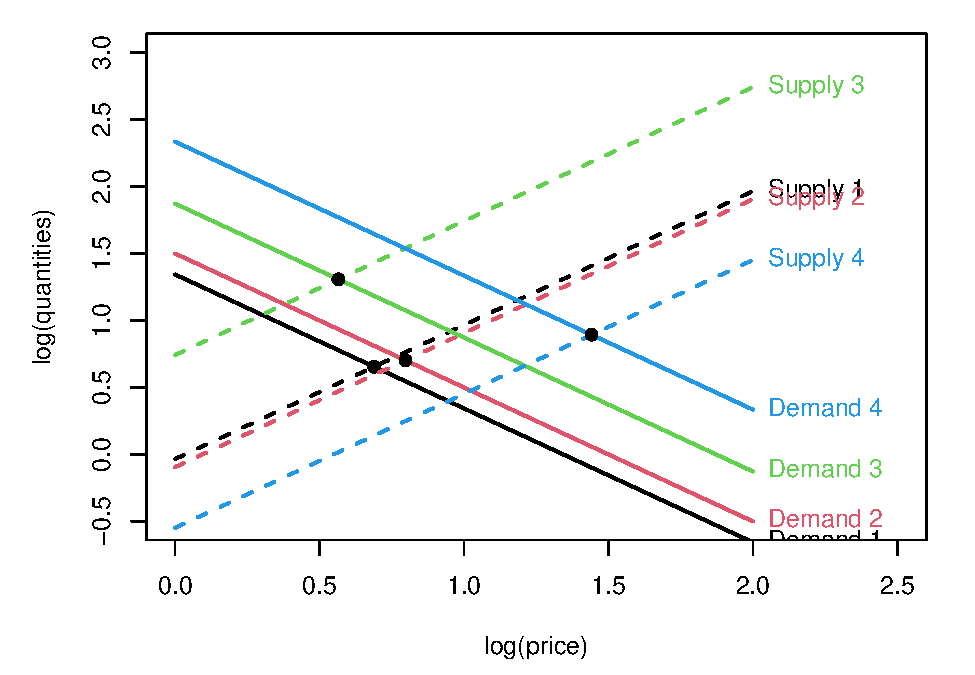
\includegraphics{AdvECTS_files/figure-latex/figureIV-1.pdf}
\caption{\label{fig:figureIV}This figure illustrates the situation prevailing when estimating a price-elasticity (and the price is endogenous).}
\end{figure}

Let us use IV regressions to estimate the price elasticity of cigarette demand. For that purpose, we use the \texttt{CigarettesSW} dataset of package \texttt{AER} (these data are used by \citet{Stock_Watson_2003}). This panel dataset documents cigarette consumption for the 48 continental US States from 1985--1995. The instrument is the real tax on cigarettes arising from the state's general sales tax. The rationale is that larger general sales tax drives cigarette prices up, but the general tax is not determined by other forces affecting \(\varepsilon_t^d\).

\begin{Shaded}
\begin{Highlighting}[]
\FunctionTok{data}\NormalTok{(}\StringTok{"CigarettesSW"}\NormalTok{, }\AttributeTok{package =} \StringTok{"AER"}\NormalTok{)}
\NormalTok{CigarettesSW}\SpecialCharTok{$}\NormalTok{rprice  }\OtherTok{\textless{}{-}} \FunctionTok{with}\NormalTok{(CigarettesSW, price}\SpecialCharTok{/}\NormalTok{cpi)}
\NormalTok{CigarettesSW}\SpecialCharTok{$}\NormalTok{rincome }\OtherTok{\textless{}{-}} \FunctionTok{with}\NormalTok{(CigarettesSW, income}\SpecialCharTok{/}\NormalTok{population}\SpecialCharTok{/}\NormalTok{cpi)}
\NormalTok{CigarettesSW}\SpecialCharTok{$}\NormalTok{tdiff   }\OtherTok{\textless{}{-}} \FunctionTok{with}\NormalTok{(CigarettesSW, (taxs }\SpecialCharTok{{-}}\NormalTok{ tax)}\SpecialCharTok{/}\NormalTok{cpi)}

\DocumentationTok{\#\# model }
\NormalTok{eq.IV1 }\OtherTok{\textless{}{-}} \FunctionTok{ivreg}\NormalTok{(}\FunctionTok{log}\NormalTok{(packs) }\SpecialCharTok{\textasciitilde{}} \FunctionTok{log}\NormalTok{(rprice) }\SpecialCharTok{+} \FunctionTok{log}\NormalTok{(rincome) }\SpecialCharTok{|} \FunctionTok{log}\NormalTok{(rincome) }\SpecialCharTok{+}\NormalTok{ tdiff }\SpecialCharTok{+} \FunctionTok{I}\NormalTok{(tax}\SpecialCharTok{/}\NormalTok{cpi),}
                \AttributeTok{data =}\NormalTok{ CigarettesSW, }\AttributeTok{subset =}\NormalTok{ year }\SpecialCharTok{==} \StringTok{"1995"}\NormalTok{)}
\NormalTok{eq.IV2 }\OtherTok{\textless{}{-}} \FunctionTok{ivreg}\NormalTok{(}\FunctionTok{log}\NormalTok{(packs) }\SpecialCharTok{\textasciitilde{}} \FunctionTok{log}\NormalTok{(rprice) }\SpecialCharTok{|}\NormalTok{ tdiff,}
                \AttributeTok{data =}\NormalTok{ CigarettesSW, }\AttributeTok{subset =}\NormalTok{ year }\SpecialCharTok{==} \StringTok{"1995"}\NormalTok{)}
\NormalTok{eq.no.IV }\OtherTok{\textless{}{-}} \FunctionTok{lm}\NormalTok{(}\FunctionTok{log}\NormalTok{(packs) }\SpecialCharTok{\textasciitilde{}} \FunctionTok{log}\NormalTok{(rprice) }\SpecialCharTok{+} \FunctionTok{log}\NormalTok{(rincome),}
               \AttributeTok{data =}\NormalTok{ CigarettesSW, }\AttributeTok{subset =}\NormalTok{ year }\SpecialCharTok{==} \StringTok{"1995"}\NormalTok{)}
\NormalTok{stargazer}\SpecialCharTok{::}\FunctionTok{stargazer}\NormalTok{(eq.no.IV,eq.IV1,eq.IV2,}\AttributeTok{type=}\StringTok{"text"}\NormalTok{,}\AttributeTok{no.space =} \ConstantTok{TRUE}\NormalTok{)}
\end{Highlighting}
\end{Shaded}

\begin{verbatim}
## 
## ==========================================================================
##                                      Dependent variable:                  
##                     ------------------------------------------------------
##                                           log(packs)                      
##                              OLS                    instrumental          
##                                                       variable            
##                              (1)                 (2)             (3)      
## --------------------------------------------------------------------------
## log(rprice)               -1.407***           -1.277***       -1.084***   
##                            (0.251)             (0.263)         (0.317)    
## log(rincome)                0.344               0.280                     
##                            (0.235)             (0.239)                    
## Constant                  10.342***           9.895***        9.720***    
##                            (1.023)             (1.059)         (1.514)    
## --------------------------------------------------------------------------
## Observations                  48                 48              48       
## R2                          0.433               0.429           0.401     
## Adjusted R2                 0.408               0.404           0.388     
## Residual Std. Error    0.187 (df = 45)     0.188 (df = 45) 0.190 (df = 46)
## F Statistic         17.165*** (df = 2; 45)                                
## ==========================================================================
## Note:                                          *p<0.1; **p<0.05; ***p<0.01
\end{verbatim}

\begin{Shaded}
\begin{Highlighting}[]
\FunctionTok{summary}\NormalTok{(eq.IV1,}\AttributeTok{diagnostics =} \ConstantTok{TRUE}\NormalTok{)}\SpecialCharTok{$}\NormalTok{diagnostics}
\end{Highlighting}
\end{Shaded}

\begin{verbatim}
##                  df1 df2   statistic      p-value
## Weak instruments   2  44 244.7337536 1.444054e-24
## Wu-Hausman         1  44   3.0678163 8.682505e-02
## Sargan             1  NA   0.3326221 5.641191e-01
\end{verbatim}

\end{example}

\begin{example}[Education and wage]
\protect\hypertarget{exm:IVCollegeDistance}{}\label{exm:IVCollegeDistance}

In this example, we make use of another dataset proposed by \citet{Stock_Watson_2003}, namely the \texttt{CollegeDistance} dataset.\footnote{Cross-section data from the High School and Beyond survey conducted by the Department of Education in the 80s. The survey includes students from approximately 1,100 high schools.} the objective is to estimate the effect of education on wages. Education choice is suspected to be an endogenous variable, which calls for an IV strategy. The instrumental variable is the distance to college.

\begin{Shaded}
\begin{Highlighting}[]
\FunctionTok{library}\NormalTok{(sem)}
\FunctionTok{data}\NormalTok{(}\StringTok{"CollegeDistance"}\NormalTok{, }\AttributeTok{package =} \StringTok{"AER"}\NormalTok{)}
\NormalTok{eq}\FloatTok{.1}\NormalTok{st.stage }\OtherTok{\textless{}{-}} \FunctionTok{lm}\NormalTok{(education }\SpecialCharTok{\textasciitilde{}}\NormalTok{ urban }\SpecialCharTok{+}\NormalTok{ gender }\SpecialCharTok{+}\NormalTok{ ethnicity }\SpecialCharTok{+}\NormalTok{ unemp }\SpecialCharTok{+}\NormalTok{ distance,}
                   \AttributeTok{data =}\NormalTok{ CollegeDistance)}
\NormalTok{CollegeDistance}\SpecialCharTok{$}\NormalTok{ed.pred}\OtherTok{\textless{}{-}} \FunctionTok{predict}\NormalTok{(eq}\FloatTok{.1}\NormalTok{st.stage)}
\NormalTok{eq}\FloatTok{.2}\NormalTok{nd.stage }\OtherTok{\textless{}{-}} \FunctionTok{lm}\NormalTok{(wage }\SpecialCharTok{\textasciitilde{}}\NormalTok{ urban }\SpecialCharTok{+}\NormalTok{ gender }\SpecialCharTok{+}\NormalTok{ ethnicity }\SpecialCharTok{+}\NormalTok{ unemp }\SpecialCharTok{+}\NormalTok{ ed.pred ,}
                   \AttributeTok{data =}\NormalTok{ CollegeDistance)}
\NormalTok{eqOLS }\OtherTok{\textless{}{-}} \FunctionTok{lm}\NormalTok{(wage }\SpecialCharTok{\textasciitilde{}}\NormalTok{ urban }\SpecialCharTok{+}\NormalTok{ gender }\SpecialCharTok{+}\NormalTok{ ethnicity }\SpecialCharTok{+}\NormalTok{ unemp }\SpecialCharTok{+}\NormalTok{ education,}
            \AttributeTok{data=}\NormalTok{CollegeDistance)}
\NormalTok{eqTSLS }\OtherTok{\textless{}{-}} \FunctionTok{ivreg}\NormalTok{(wage }\SpecialCharTok{\textasciitilde{}}\NormalTok{ urban }\SpecialCharTok{+}\NormalTok{ gender }\SpecialCharTok{+}\NormalTok{ ethnicity }\SpecialCharTok{+}\NormalTok{ unemp }\SpecialCharTok{+}\NormalTok{ education}\SpecialCharTok{|}
\NormalTok{                  urban }\SpecialCharTok{+}\NormalTok{ gender }\SpecialCharTok{+}\NormalTok{ ethnicity }\SpecialCharTok{+}\NormalTok{ unemp }\SpecialCharTok{+}\NormalTok{ distance,}
                \AttributeTok{data=}\NormalTok{CollegeDistance)}
\NormalTok{stargazer}\SpecialCharTok{::}\FunctionTok{stargazer}\NormalTok{(eq}\FloatTok{.1}\NormalTok{st.stage,eq}\FloatTok{.2}\NormalTok{nd.stage,eqTSLS,eqOLS,}\AttributeTok{type=}\StringTok{"text"}\NormalTok{,}\AttributeTok{no.space =} \ConstantTok{TRUE}\NormalTok{)}
\end{Highlighting}
\end{Shaded}

\begin{verbatim}
## 
## ===========================================================================
##                                             Dependent variable:            
##                                 -------------------------------------------
##                                 education               wage               
##                                    OLS       OLS     instrumental    OLS   
##                                                        variable            
##                                    (1)       (2)         (3)         (4)   
## ---------------------------------------------------------------------------
## urbanyes                         -0.092     0.046       0.046       0.070  
##                                  (0.065)   (0.045)     (0.060)     (0.045) 
## genderfemale                     -0.025    -0.071*      -0.071    -0.085** 
##                                  (0.052)   (0.037)     (0.050)     (0.037) 
## ethnicityafam                   -0.524*** -0.227***    -0.227**   -0.556***
##                                  (0.072)   (0.073)     (0.099)     (0.052) 
## ethnicityhispanic               -0.275*** -0.351***   -0.351***   -0.544***
##                                  (0.068)   (0.057)     (0.077)     (0.049) 
## unemp                             0.010    0.139***    0.139***   0.133*** 
##                                  (0.010)   (0.007)     (0.009)     (0.007) 
## distance                        -0.087***                                  
##                                  (0.012)                                   
## ed.pred                                    0.647***                        
##                                            (0.101)                         
## education                                              0.647***     0.005  
##                                                        (0.136)     (0.010) 
## Constant                        14.061***   -0.359      -0.359    8.641*** 
##                                  (0.083)   (1.412)     (1.908)     (0.157) 
## ---------------------------------------------------------------------------
## Observations                      4,739     4,739       4,739       4,739  
## R2                                0.023     0.117       -0.612      0.110  
## Adjusted R2                       0.022     0.116       -0.614      0.109  
## Residual Std. Error (df = 4732)   1.770     1.263       1.706       1.268  
## F Statistic (df = 6; 4732)      18.552*** 104.971***              97.274***
## ===========================================================================
## Note:                                           *p<0.1; **p<0.05; ***p<0.01
\end{verbatim}

\end{example}

\hypertarget{general-regression-model-grm-and-robust-covariance-matrices}{%
\section{General Regression Model (GRM) and robust covariance matrices}\label{general-regression-model-grm-and-robust-covariance-matrices}}

The statistical inference presented above relies on strong assumptions regarding the stochastic properties of the errors. Namely, they are assumed to be mutually uncorrelated (Hypothesis @ref(hyp:noncorrel\_resid)) and homoskedastic (Hypothesis \ref{hyp:homoskedasticity}.

The objective of this section is to present approaches aimed at adjusting the estimate of the covariance matrix of the OLS estimator (\((\mathbf{X}'\mathbf{X})^{-1}s^2\), see Eq. \eqref{eq:sXX}), when the previous hypotheses do not hold.

\hypertarget{presentation-of-the-general-regression-model-grm}{%
\subsection{Presentation of the General Regression Model (GRM)}\label{presentation-of-the-general-regression-model-grm}}

It will prove useful to introduce the following notation:
\begin{eqnarray}
\mathbb{V}ar(\boldsymbol\varepsilon | \mathbf{X}) = \mathbb{E}(\boldsymbol\varepsilon \boldsymbol\varepsilon'| \mathbf{X}) &=& \boldsymbol\Sigma. \label{eq:assumGLS2}
\end{eqnarray}

Note that Eq. (\eqref{eq:assumGLS2}) is more general than Hypothesis \ref{hyp:homoskedasticity} and @ref(hyp:noncorrel\_resid) because the diagonal entries of \(\boldsymbol\Sigma\) may be different (as opposed to under Hypothesis \ref{hyp:homoskedasticity}), and the non-diagonal entries of \(\boldsymbol\Sigma\) can be non-null (as opposed to under Hypothesis \ref{hyp:noncorrelResid}).

\begin{definition}[General Regression Model (GRM)]
\protect\hypertarget{def:GRM}{}\label{def:GRM}Hypothesis \ref{hyp:fullrank} and \ref{hyp:exogeneity}, together with Eq. \eqref{eq:assumGLS2}, form the General Regression Model (GRM) framework.
\end{definition}

Naturally, a regression model where Hypotheses \ref{hyp:fullrank} to \ref{hyp:noncorrelResid} hold is a specific case of the GRM framework.

The GRM context notably encompasses situations of heteroskedasticity and autocorrelation:

\begin{itemize}
\item
  Heteroskedasticity:
  \begin{equation}
  \boldsymbol\Sigma = \left[  \begin{array}{cccc}
  \sigma_1^2 & 0 & \dots & 0 \\
  0 & \sigma_2^2 &  & 0 \\
  \vdots && \ddots& \vdots \\
  0 & \dots & 0 & \sigma_n^2
  \end{array} \right]. \label{eq:heteroskedasticity}
  \end{equation}
\item
  Autocorrelation:
  \begin{equation}
  \boldsymbol\Sigma = \sigma^2 \left[ \begin{array}{cccc}
  1 & \rho_{2,1} & \dots & \rho_{n,1} \\
  \rho_{2,1} & 1 &  & \vdots \\
  \vdots && \ddots& \rho_{n,n-1} \\
  \rho_{n,1} & \rho_{n,2} & \dots & 1
  \end{array} \right]. \label{eq:autocorrelation}
  \end{equation}
\end{itemize}

\begin{example}[Auto-regressive processes]
\protect\hypertarget{exm:autocorrelaaa}{}\label{exm:autocorrelaaa}Autocorrelation is, in particular, a recurrent problem when time-series data are used (see Section \ref{TS}).

In a time-series context, subscript \(i\) refers to a date. Assume for instance that:
\begin{equation}
y_i = \mathbf{x}_i' \boldsymbol\beta + \varepsilon_i \label{eq:usual}
\end{equation}
with
\begin{equation}
\varepsilon_i = \rho \varepsilon_{i-1} + v_i, \quad v_i \sim \mathcal{N}(0,\sigma_v^2).\label{eq:usual2}
\end{equation}
In this case, we are in the GRM context, with:
\begin{equation}\label{eq:SigmaAutocorrel}
\boldsymbol\Sigma =\frac{ \sigma_v^2}{1 - \rho^2} \left[    \begin{array}{cccc}
1 & \rho & \dots & \rho^{n-1} \\
\rho & 1 &  & \vdots \\
\vdots && \ddots& \rho \\
\rho^{n-1} & \rho^{n-2} & \dots & 1
\end{array} \right].
\end{equation}
\end{example}

In some cases ---in particular when one assumes a parametric formulation for \(\boldsymbol\Sigma\)--- one can determine a better (more accurate) estimator than the OLS one. This approach is called Generalized Least Squares (GLS), which we present below.

\hypertarget{GLS}{%
\subsection{Generalized Least Squares}\label{GLS}}

Assume \(\boldsymbol\Sigma\) is known (``feasible GLS''). Because \(\boldsymbol\Sigma\) is symmetric positive, it admits a spectral decomposition of the form \(\boldsymbol\Sigma = \mathbf{C} \boldsymbol\Lambda \mathbf{C}'\), where \(\mathbf{C}\) is an orthogonal matrix (i.e.~\(\mathbf{C}\mathbf{C}'=Id\)) and \(\boldsymbol\Lambda\) is a diagonal matrix (the diagonal entries are the eigenvalues of \(\boldsymbol\Sigma\)).

We have \(\boldsymbol\Sigma = (\mathbf{P}\mathbf{P}')^{-1}\) with \(\mathbf{P} = \mathbf{C}\boldsymbol\Lambda^{-1/2}\). Consider the transformed model:
\[
\mathbf{P}'\mathbf{y} = \mathbf{P}'\mathbf{X}\boldsymbol\beta + \mathbf{P}'\boldsymbol\varepsilon \quad \mbox{or} \quad \mathbf{y}^* = \mathbf{X}^*\boldsymbol\beta + \boldsymbol\varepsilon^*.
\]
The variance of \(\boldsymbol\varepsilon^*\) is \(\mathbf{I}\). In the transformed model, OLS is BLUE (Gauss-Markow Theorem \ref{thm:GaussMarkov}).

The \textbf{Generalized least squares} estimator of \(\boldsymbol\beta\) is:
\begin{equation}
\boxed{\mathbf{b}_{GLS} = (\mathbf{X}'\boldsymbol\Sigma^{-1}\mathbf{X})^{-1}\mathbf{X}'\boldsymbol\Sigma^{-1}\mathbf{y}}.\label{eq:betaGLS}
\end{equation}
We have:
\[
\mathbb{V}ar(\mathbf{b}_{GLS}|\mathbf{X}) = (\mathbf{X}'\boldsymbol\Sigma^{-1}\mathbf{X})^{-1}.
\]

However, in general, \(\boldsymbol\Sigma\) is unknown. The GLS estimator is then said to be \emph{infeasible}. Some structure is required. Assume \(\boldsymbol\Sigma\) admits a parametric form \(\boldsymbol\Sigma(\theta)\). The estimation becomes \emph{feasible} (FGLS) if one replaces \(\boldsymbol\Sigma(\theta)\) by \(\boldsymbol\Sigma(\hat\theta)\), where \(\hat\theta\) is a consistent estimator of \(\theta\). In that case, the FGLS is asymptotically efficient (see Example \ref{exm:autocorrelaa}).

When \(\boldsymbol\Sigma\) has no obvious structure: the OLS (or IV) is the only estimator available. Under regularity assumptions, it remains unbiased, consistent, and asymptotically normally distributed, but not efficient. Standard inference procedures are no longer appropriate.

\begin{example}[GLS in the auto-correlation case]
\protect\hypertarget{exm:autocorrelaaa2}{}\label{exm:autocorrelaaa2}Consider the case presented in Example \ref{exm:autocorrelaaa}. Because the OLS estimate \(\mathbf{b}\) of \(\boldsymbol\beta\) is consistent, the estimates \(e_i\)s of the \(\varepsilon_i\)s also are. Consistent estimators of \(\rho\) and \(\sigma_v\) are then obtained by regressing the \(e_i\)s on the \(e_{i-1}\)s. Using these estimates in Eq. \eqref{eq:SigmaAutocorrel} provides a consistent estimate of \(\boldsymbol\Sigma\). Applying these steps recursively gives an efficient estimator of \(\boldsymbol\beta\) (\citet{Cochrane_Orcutt_1949}).
\end{example}

\hypertarget{asymptotic-properties-of-the-ols-estimator-in-the-grm-framework}{%
\subsection{Asymptotic properties of the OLS estimator in the GRM framework}\label{asymptotic-properties-of-the-ols-estimator-in-the-grm-framework}}

In the GRM framework, we have:
\begin{equation}
\mathbb{V}ar(\mathbf{b}|\mathbf{X}) = \frac{1}{n}\left(\frac{1}{n}\mathbf{X}'\mathbf{X}\right)^{-1}\left(\frac{1}{n}\mathbf{X}'\boldsymbol\Sigma\mathbf{X}\right)\left(\frac{1}{n}\mathbf{X}'\mathbf{X}\right)^{-1}.\label{eq:xsx}
\end{equation}

The conditional covariance matrix of the OLS estimator is therefore not \(\sigma^2 (\mathbf{X}'\mathbf{X})^{-1}\) any longer Therefore, using \(s^2 (\mathbf{X}'\mathbf{X})^{-1}\) for inference may be misleading. Below, we will see appropriate how to construct appropriate estimates of the covariance matrix of \(\mathbf{b}\). Before, that, let us prove that the OLS estimator remains consistent in the GRM framework.

\begin{proposition}[Consistency of the OLS estimator in the GRM framework]
\protect\hypertarget{prp:XXX}{}\label{prp:XXX}If \(\mbox{plim }(\mathbf{X}'\mathbf{X}/n)\) and \(\mbox{plim }(\mathbf{X}'\boldsymbol\Sigma\mathbf{X}/n)\) are finite positive definite matrices, then \(\mbox{plim }(\mathbf{b})=\boldsymbol\beta\).
\end{proposition}

\begin{proof}
We have \(\mathbb{V}ar(\mathbf{b})=\mathbb{E}[\mathbb{V}ar(\mathbf{b}|\mathbf{X})]+\mathbb{V}ar[\mathbb{E}(\mathbf{b}|\mathbf{X})]\). Since \(\mathbb{E}(\mathbf{b}|\mathbf{X})=\boldsymbol\beta\), \(\mathbb{V}ar[\mathbb{E}(\mathbf{b}|\mathbf{X})]=0\). Eq. \eqref{eq:xsx} implies that \(\mathbb{V}ar(\mathbf{b}|\mathbf{X}) \rightarrow 0\). Hence \(\mathbf{b}\) converges in mean square, and therefore in probability (see Prop. \ref{implicationsconv}).
\end{proof}

Prop. \ref{prp:AsymptGRM} gives the asymptotic distribution of the OLS estimator in the GRM framework.

\begin{proposition}[Asymptotic distribution of the OLS estimator in the GRM framework]
\protect\hypertarget{prp:AsymptGRM}{}\label{prp:AsymptGRM}If \(Q_{xx}=\mbox{plim }(\mathbf{X}'\mathbf{X}/n)\) and \(Q_{x\boldsymbol\Sigma x}=\mbox{plim }(\mathbf{X}'\boldsymbol\Sigma\mathbf{X}/n)\) are finite positive definite matrices, then:
\[
\sqrt{n}(\mathbf{b}-\boldsymbol\beta) \overset{d}{\rightarrow} \mathcal{N}(0,Q_{xx}^{-1}Q_{x\boldsymbol\Sigma x}Q_{xx}^{-1}).
\]
\end{proposition}

The IV estimator also features a normal asymptotic distribution:

\begin{proposition}[Asymptotic distribution of the OLS estimator in the GRM framework]
\protect\hypertarget{prp:AsymptIVGRM}{}\label{prp:AsymptIVGRM}If regressors and IV variables are ``well-behaved'', then:
\[
\mathbf{b}_{iv} \overset{a}{\sim} \mathcal{N}(\boldsymbol\beta,\mathbf{V}_{iv}),
\]
where
\[
\mathbf{V}_{iv} = \frac{1}{n}(\mathbf{Q}^*)\mbox{ plim }\left(\frac{1}{n} \mathbf{Z}'\boldsymbol\Sigma \mathbf{Z}\right)(\mathbf{Q}^*)',
\]
with
\[
\mathbf{Q}^* = [\mathbf{Q}_{xz}\mathbf{Q}_{zz}^{-1}\mathbf{Q}_{zx}]^{-1}\mathbf{Q}_{xz}\mathbf{Q}_{zz}^{-1}.
\]
\end{proposition}

For practical purposes, one needs to have estimates of \(\boldsymbol\Sigma\) in Props. \ref{prp:AsymptGRM} or \ref{prp:AsymptIVGRM}. The complication comes from the fact that \(\boldsymbol\Sigma\) is of dimension \(n \times n\), and its estimation ---based on a sample of length \(n\)--- is therefore infeasible in the general case. Notwithstanding, looking at Eq. \eqref{eq:xsx}, it appears that one can focus on the estimation of \(Q_{x\boldsymbol\Sigma x}=\mbox{plim }(\mathbf{X}'\boldsymbol\Sigma\mathbf{X}/n)\) (or \(\mbox{plim }\left(\frac{1}{n} \mathbf{Z}'\boldsymbol\Sigma \mathbf{Z}\right)\) in the IV case). This matrix being of dimension \(K \times K\), its estimation is easier.

We have:
\begin{equation}
\frac{1}{n}\mathbf{X}'\boldsymbol\Sigma\mathbf{X} = \frac{1}{n}\sum_{i=1}^{n}\sum_{j=1}^{n}\sigma_{i,j}\mathbf{x}_i\mathbf{x}'_j. \label{eq:GeneralXSigmaX}
\end{equation}

The so-called \textbf{robust covariance matrices} are estimates of the previous matrix. Their computation is based on the fact that if \(\mathbf{b}\) is consistent, then the \(e_i\)'s are consistent (pointwise) estimators of the \(\varepsilon_i\)'s. Let us present such robust covariance matrices in two basic situations: heteroskedasticity (Example \ref{exm:HCheteroskedasticity}) and auto-correlation of the residuals (Example \ref{exm:})

\begin{example}[Heteroskedasticity]
\protect\hypertarget{exm:HCheteroskedasticity}{}\label{exm:HCheteroskedasticity}This is the case of Eq. \eqref{eq:heteroskedasticity}.

We then need to estimate \(\frac{1}{n}\sum_{i=1}^{n}\sigma_{i}^2\mathbf{x}_i\mathbf{x}'_i\). \citet{White_1980}: Under general conditions:
\begin{equation}
\mbox{plim}\left( \frac{1}{n}\sum_{i=1}^{n}\sigma_{i}^2\mathbf{x}_i\mathbf{x}'_i \right) = 
\mbox{plim}\left( \frac{1}{n}\sum_{i=1}^{n}e_{i}^2\mathbf{x}_i\mathbf{x}'_i \right). \label{eq:white}
\end{equation}
The estimator of \(\frac{1}{n}\mathbf{X}'\boldsymbol\Sigma\mathbf{X}\) therefore is:
\begin{equation}
\frac{1}{n}\mathbf{X}'\mathbf{E}^2\mathbf{X},\label{eq:White}
\end{equation}
where \(\mathbf{E}\) is an \(n \times n\) diagonal matrix whose diagonal elements are the estimated residuals \(e_i\).

Illustration: Figure \ref{fig:exmpSalarayPhD}.

Let us illustrate the influence of heteroskedasticity using simulations.

We consider the following model:
\[
y_i = x_i + \varepsilon_i, \quad \varepsilon_i \sim \mathcal{N}(0,x_i^2).
\]
where the \(x_i\)s are i.i.d. \(t(4)\).

Here is a simulated sample (\(n=200\)) of this model:

\begin{Shaded}
\begin{Highlighting}[]
\NormalTok{n }\OtherTok{\textless{}{-}} \DecValTok{200}
\NormalTok{x }\OtherTok{\textless{}{-}} \FunctionTok{rt}\NormalTok{(n,}\AttributeTok{df=}\DecValTok{5}\NormalTok{)}
\NormalTok{y }\OtherTok{\textless{}{-}}\NormalTok{ x }\SpecialCharTok{+}\NormalTok{ x}\SpecialCharTok{*}\FunctionTok{rnorm}\NormalTok{(n)}
\FunctionTok{plot}\NormalTok{(x,y,}\AttributeTok{pch=}\DecValTok{19}\NormalTok{)}
\end{Highlighting}
\end{Shaded}

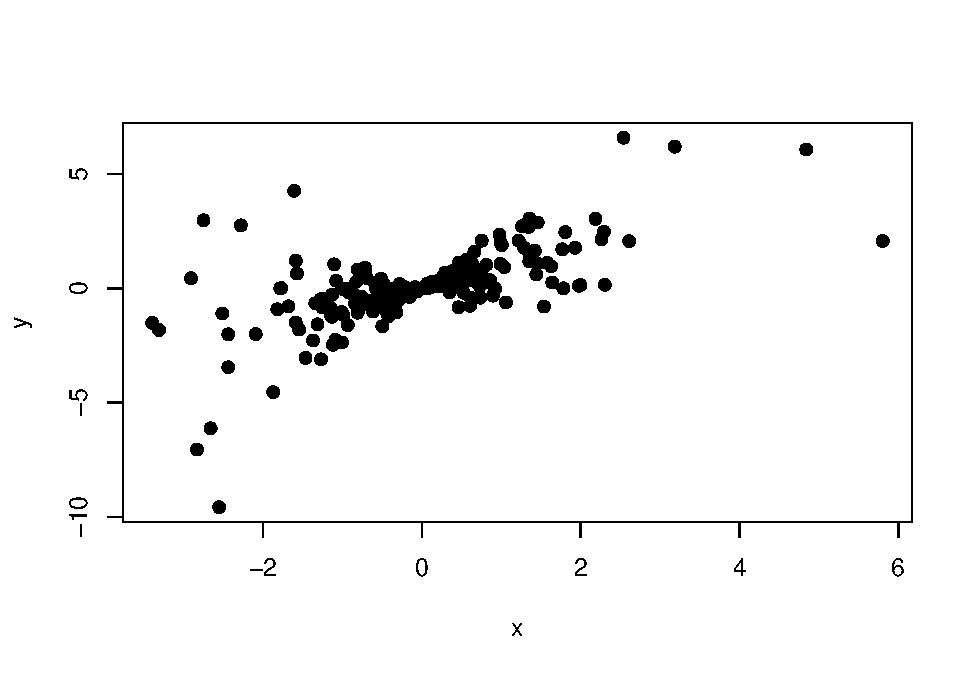
\includegraphics{AdvECTS_files/figure-latex/simulHeterosk-1.pdf}

We simulate 1000 samples of the same model with \(n=200\). For each sample, we compute the OLS estimate of \(\beta\) (=1). Using these 1000 estimates of \(b\), we construct an approximated \emph{(kernel-based) distribution of this OLS estimator} (in red on the figure).

For each of the 1000 OLS estimations, we employ \emph{the standard OLS variance formula (\(s^2 (\mathbf{X}'\mathbf{X})^{-1}\))} to estimate the variance of \(b\). The blue curve is a normal distribution centred on 1 and whose variance is the average of the 1000 previous variance estimates.

The variance of the simulated \(b\) is of 0.040 (that is the \emph{true} one); the average of the estimated variances based on the standard OLS formula is of 0.005 (\emph{bad} estimate); the average of the estimated variances based on the White robust covariance matrix is of 0.030 (better estimate).

The standard OLS formula for the variance of \(b\) overestimates the precision of this estimator.

For almost 50\% of the simulations, 1 is not included in the 95\% confidence interval of \(\beta\) when the computation of the interval is based on the standard OLS formula for the variance of \(b\).

When the White robust covariance matrix is used, 1 is not in the 95\% confidence interval of \(\beta\) for less than 10\% of the simulations.

\begin{Shaded}
\begin{Highlighting}[]
\NormalTok{n }\OtherTok{\textless{}{-}} \DecValTok{200}
\NormalTok{N }\OtherTok{\textless{}{-}} \DecValTok{1000}
\NormalTok{XX }\OtherTok{\textless{}{-}} \FunctionTok{matrix}\NormalTok{(}\FunctionTok{rt}\NormalTok{(n}\SpecialCharTok{*}\NormalTok{N,}\AttributeTok{df=}\DecValTok{5}\NormalTok{),n,N)}
\NormalTok{YY }\OtherTok{\textless{}{-}} \FunctionTok{matrix}\NormalTok{(XX }\SpecialCharTok{+}\NormalTok{ XX}\SpecialCharTok{*}\FunctionTok{rnorm}\NormalTok{(n),n,N)}
\NormalTok{all\_b       }\OtherTok{\textless{}{-}} \ConstantTok{NULL}
\NormalTok{all\_V\_OLS   }\OtherTok{\textless{}{-}} \ConstantTok{NULL}
\NormalTok{all\_V\_White }\OtherTok{\textless{}{-}} \ConstantTok{NULL}
\ControlFlowTok{for}\NormalTok{(j }\ControlFlowTok{in} \DecValTok{1}\SpecialCharTok{:}\NormalTok{N)\{}
\NormalTok{  Y }\OtherTok{\textless{}{-}} \FunctionTok{matrix}\NormalTok{(YY[,j],}\AttributeTok{ncol=}\DecValTok{1}\NormalTok{)}
\NormalTok{  X }\OtherTok{\textless{}{-}} \FunctionTok{matrix}\NormalTok{(XX[,j],}\AttributeTok{ncol=}\DecValTok{1}\NormalTok{)}
\NormalTok{  b }\OtherTok{\textless{}{-}} \FunctionTok{solve}\NormalTok{(}\FunctionTok{t}\NormalTok{(X)}\SpecialCharTok{\%*\%}\NormalTok{X) }\SpecialCharTok{\%*\%} \FunctionTok{t}\NormalTok{(X)}\SpecialCharTok{\%*\%}\NormalTok{Y}
\NormalTok{  e }\OtherTok{\textless{}{-}}\NormalTok{ Y }\SpecialCharTok{{-}}\NormalTok{ X }\SpecialCharTok{\%*\%}\NormalTok{ b}
\NormalTok{  S }\OtherTok{\textless{}{-}} \DecValTok{1}\SpecialCharTok{/}\NormalTok{n }\SpecialCharTok{*} \FunctionTok{t}\NormalTok{(X) }\SpecialCharTok{\%*\%} \FunctionTok{diag}\NormalTok{(}\FunctionTok{c}\NormalTok{(e}\SpecialCharTok{\^{}}\DecValTok{2}\NormalTok{)) }\SpecialCharTok{\%*\%}\NormalTok{ X}
\NormalTok{  V\_OLS   }\OtherTok{\textless{}{-}} \FunctionTok{solve}\NormalTok{(}\FunctionTok{t}\NormalTok{(X)}\SpecialCharTok{\%*\%}\NormalTok{X) }\SpecialCharTok{*} \FunctionTok{var}\NormalTok{(e)}
\NormalTok{  V\_White }\OtherTok{\textless{}{-}} \DecValTok{1}\SpecialCharTok{/}\NormalTok{n }\SpecialCharTok{*}\NormalTok{ (}\FunctionTok{solve}\NormalTok{(}\DecValTok{1}\SpecialCharTok{/}\NormalTok{n}\SpecialCharTok{*}\FunctionTok{t}\NormalTok{(X)}\SpecialCharTok{\%*\%}\NormalTok{X)) }\SpecialCharTok{\%*\%}\NormalTok{ S }\SpecialCharTok{\%*\%}\NormalTok{ (}\FunctionTok{solve}\NormalTok{(}\DecValTok{1}\SpecialCharTok{/}\NormalTok{n}\SpecialCharTok{*}\FunctionTok{t}\NormalTok{(X)}\SpecialCharTok{\%*\%}\NormalTok{X))}
  
\NormalTok{  all\_b       }\OtherTok{\textless{}{-}} \FunctionTok{c}\NormalTok{(all\_b,b)}
\NormalTok{  all\_V\_OLS   }\OtherTok{\textless{}{-}} \FunctionTok{c}\NormalTok{(all\_V\_OLS,V\_OLS)}
\NormalTok{  all\_V\_White }\OtherTok{\textless{}{-}} \FunctionTok{c}\NormalTok{(all\_V\_White,V\_White)}
\NormalTok{\}}
\FunctionTok{plot}\NormalTok{(}\FunctionTok{density}\NormalTok{(all\_b))}
\FunctionTok{abline}\NormalTok{(}\AttributeTok{v=}\FunctionTok{mean}\NormalTok{(all\_b),}\AttributeTok{lty=}\DecValTok{2}\NormalTok{)}
\FunctionTok{abline}\NormalTok{(}\AttributeTok{v=}\DecValTok{1}\NormalTok{)}
\NormalTok{x }\OtherTok{\textless{}{-}} \FunctionTok{seq}\NormalTok{(}\DecValTok{0}\NormalTok{,}\DecValTok{2}\NormalTok{,}\AttributeTok{by=}\NormalTok{.}\DecValTok{01}\NormalTok{)}
\FunctionTok{lines}\NormalTok{(x,}\FunctionTok{dnorm}\NormalTok{(x,}\AttributeTok{mean =} \DecValTok{1}\NormalTok{,}\AttributeTok{sd =} \FunctionTok{mean}\NormalTok{(}\FunctionTok{sqrt}\NormalTok{(all\_V\_OLS))),}\AttributeTok{col=}\StringTok{"blue"}\NormalTok{)}
\FunctionTok{lines}\NormalTok{(x,}\FunctionTok{dnorm}\NormalTok{(x,}\AttributeTok{mean =} \DecValTok{1}\NormalTok{,}\AttributeTok{sd =} \FunctionTok{mean}\NormalTok{(}\FunctionTok{sqrt}\NormalTok{(all\_V\_White))),}\AttributeTok{col=}\StringTok{"red"}\NormalTok{)}
\end{Highlighting}
\end{Shaded}

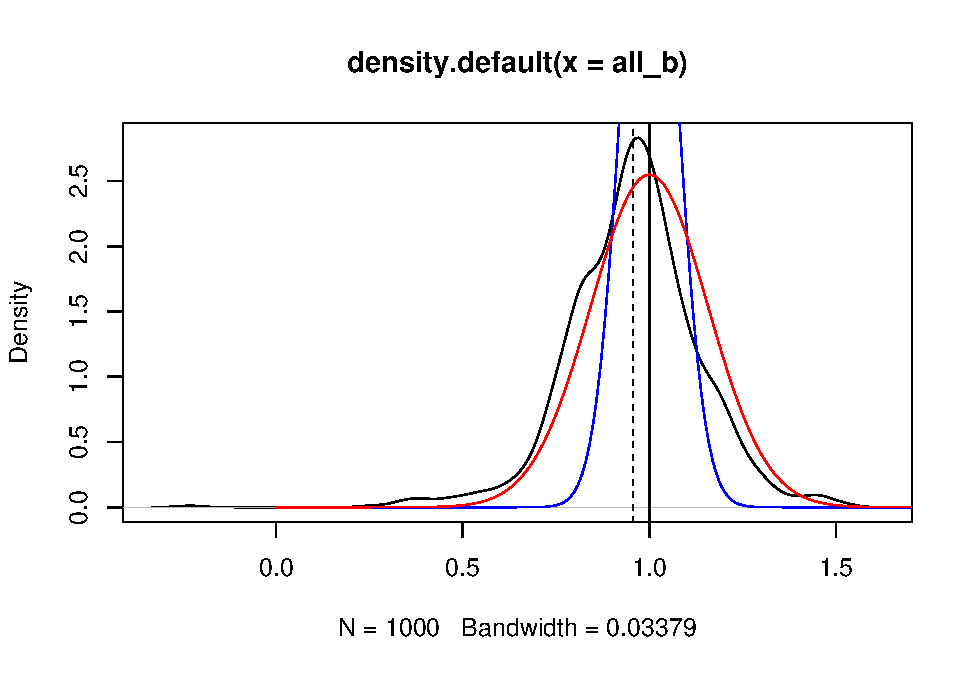
\includegraphics{AdvECTS_files/figure-latex/simulHeterosk2-1.pdf}
\end{example}

\begin{example}[Heteroskedasticity and Autocorrelation (HAC)]
\protect\hypertarget{exm:HCheterAC}{}\label{exm:HCheterAC}This includes the cases of Eqs. \eqref{eq:heteroskedasticity} and \eqref{eq:autocorrelation}.

\href{http://www.jstor.org/stable/1913610}{Newey and West (1987)}: If the correlation between terms \(i\) and \(j\) gets sufficiently small when \(|i-j|\) increases:
\begin{eqnarray}
&&\mbox{plim} \left( \frac{1}{n}\sum_{i=1}^{n}\sum_{j=1}^{n}\sigma_{i,j}\mathbf{x}_i\mathbf{x}'_j \right) =  \\
&&\mbox{plim} \left( \frac{1}{n}\sum_{t=1}^{n}e_{t}^2\mathbf{x}_t\mathbf{x}'_t +
\frac{1}{n}\sum_{\ell=1}^{L}\sum_{t=\ell+1}^{n}w_\ell e_{t}e_{t-\ell}(\mathbf{x}_t\mathbf{x}'_{t-\ell} + \mathbf{x}_{t-\ell}\mathbf{x}'_{t})
\right) \nonumber \label{eq:NW}
\end{eqnarray}
where \(w_\ell = 1 - \ell/(L+1)\).

Let us illustrate the influence of autocorrelation using simulations.

We consider the following model:
\begin{equation}
y_i = x_i + \varepsilon_i, \quad \varepsilon_i \sim \mathcal{N}(0,x_i^2),\label{eq:simul11}
\end{equation}
where the \(x_i\)s and the \(\varepsilon_i\)s are such that:
\begin{equation}
x_i = 0.8 x_{i-1} + u_i \quad and \quad \varepsilon_i = 0.8 \varepsilon_{i-1} + v_i, \label{eq:simul22}
\end{equation}
where the \(u_i\)s and the \(v_i\)s are i.i.d. \(\mathcal{N}(0,1)\).

Here is a simulated sample (\(n=200\)) of this model:

We simulate 1000 samples of the same model with \(n=200\).

For each sample, we compute the OLS estimate of \(\beta\) (=1).

Using these 1000 estimates of \(b\), we construct an approximated (kernel-based) distribution of this OLS estimator (in red on the figure).

For each of the 1000 OLS estimations, we employ the standard OLS variance formula (\(s^2 (\mathbf{X}'\mathbf{X})^{-1}\)) to estimate the variance of \(b\). The blue curve is a normal distribution centred on 1 and whose variance is the average of the 1000 previous variance estimates.

The variance of the simulated \(b\) is of 0.020 (that is the \emph{true} one); the average of the estimated variances based on the standard OLS formula is of 0.005 (\emph{bad} estimate); the average of the estimated variances based on the White robust covariance matrix is of 0.015 (\emph{better} estimate).

The standard OLS formula for the variance of \(b\) overestimates the precision of this estimator.

For about 35\% of the simulations, 1 is not included in the 95\% confidence interval of \(\beta\) when the computation of the interval is based on the standard OLS formula for the variance of \(b\).

When the Newey-West robust covariance matrix is used, 1 is not in the 95\% confidence interval of \(\beta\) for about 13\% of the simulations.

For the sake of comparison, let us consider a model with no auto-correlation (\(x_i \sim i.i.d. \mathcal{N}(0,2.8)\) and \(\varepsilon_i \sim i.i.d. \mathcal{N}(0,2.8)\)).
\end{example}

\hypertarget{how-to-detect-autocorrelation-in-residuals}{%
\subsection{How to detect autocorrelation in residuals?}\label{how-to-detect-autocorrelation-in-residuals}}

Consider the usual regression (say Eq. \eqref{eq:usual}).

The \textbf{Durbin-Watson test} is a typical autocorrelation test. Its test statistic is:
\[
DW = \frac{\sum_{i=2}^{n}(e_i - e_{i-1})^2}{\sum_{i=1}^{n}e_i^2}= 2(1 - r) - \underbrace{\frac{e_1^2 + e_n^2}{\sum_{i=1}^{n}e_i^2}}_{\overset{p}{\rightarrow} 0},
\]
where \(r\) is the slope in the regression of the \(e_i\)s on the \(e_{i-1}\)s, i.e.:
\[
r = \frac{\sum_{i=2}^{n}e_i e_{i-1}}{\sum_{i=1}^{n-1}e_i^2}.
\]
(\(r\) is a consistent estimator of \(\mathbb{C}or(\varepsilon_i,\varepsilon_{i-1})\), i.e.~\(\rho\) in Eq. \eqref{eq:usual2}.)

Critical values depend only on T and K: see e.g.~\href{http://web.stanford.edu/~clint/bench/dwcrit.htm}{tables} CHECK.

The one-sided test for \(H_0\): \(\rho=0\) against \(H_1\): \(\rho>0\) is carried out by comparing \(DW\) to values \(d_L(T, K)\) and \(d_U(T, K)\):
\[
\left\{
\begin{array}{ll}
\mbox{If $DW < d_L$,}&\mbox{ the null hypothesis is rejected;}\\
\mbox{if $DW > d_U$,}&\mbox{ the hypothesis is not rejected;}\\
\mbox{If $d_L \le DW \le d_U$,} &\mbox{ no conclusion is drawn.}
\end{array}
\right.
\]

\hypertarget{summary}{%
\section{Summary}\label{summary}}

\begin{longtable}[]{@{}
  >{\raggedright\arraybackslash}p{(\columnwidth - 12\tabcolsep) * \real{0.1399}}
  >{\raggedright\arraybackslash}p{(\columnwidth - 12\tabcolsep) * \real{0.1062}}
  >{\raggedright\arraybackslash}p{(\columnwidth - 12\tabcolsep) * \real{0.1580}}
  >{\raggedright\arraybackslash}p{(\columnwidth - 12\tabcolsep) * \real{0.1192}}
  >{\raggedright\arraybackslash}p{(\columnwidth - 12\tabcolsep) * \real{0.1606}}
  >{\raggedright\arraybackslash}p{(\columnwidth - 12\tabcolsep) * \real{0.1244}}
  >{\raggedright\arraybackslash}p{(\columnwidth - 12\tabcolsep) * \real{0.1917}}@{}}
\toprule()
\begin{minipage}[b]{\linewidth}\raggedright
\end{minipage} & \begin{minipage}[b]{\linewidth}\raggedright
Under Assumptions \ref{hyp:fullrank}+
\end{minipage} & \begin{minipage}[b]{\linewidth}\raggedright
\(\mathbf{b}\) normal in small sample (Eq. \eqref{eq:distriBcondi})
\end{minipage} & \begin{minipage}[b]{\linewidth}\raggedright
\(\mathbf{b}\) is BLUE (Thm \ref{thm:GaussMarkov})
\end{minipage} & \begin{minipage}[b]{\linewidth}\raggedright
\(\mathbf{b}\) unbiased in small sample (Prop. \ref{prp:propOLS})
\end{minipage} & \begin{minipage}[b]{\linewidth}\raggedright
\(\mathbf{b}\) consistent (Prop. \ref{prp:XXX})\(^*\)
\end{minipage} & \begin{minipage}[b]{\linewidth}\raggedright
\(\mathbf{b}\) \(\sim\) normal in large sample (Prop. \ref{prp:AsymptGRM})\(^*\)
\end{minipage} \\
\midrule()
\endhead
\rotatebox[origin=c]{90}{ Condit. mean-zero} & \ref{hyp:exogeneity} & X & X & X & X & X \\
\rotatebox[origin=c]{90}{ Homoskedasticity} & \ref{hyp:homoskedasticity} & X & X & & & \\
\rotatebox[origin=c]{90}{Uncorrelated residuals} & \ref{hyp:noncorrelResid} & X & X & & & \\
\rotatebox[origin=c]{90}{ Normality of disturbances} & \ref{hyp:normality} & X & & & & \\
\bottomrule()
\end{longtable}

\(^*\): see however Prop. \ref{prp:XXX} and Prop. \ref{prp:AsymptGRM} for additional hypotheses. Specifically \(\mathbf{X}'\mathbf{X}/n\) and \(\mathbf{X}'\boldsymbol{\Sigma}\mathbf{X}/n\) must converge in proba. to finite positive definite matrices (\(\boldsymbol\Sigma\) is defined in Eq. \eqref{eq:assumGLS2}).

\hypertarget{clusters}{%
\section{Clusters}\label{clusters}}

\begin{Shaded}
\begin{Highlighting}[]
\FunctionTok{library}\NormalTok{(AEC)}
\FunctionTok{library}\NormalTok{(sandwich)}
\NormalTok{shp}\SpecialCharTok{$}\NormalTok{income }\OtherTok{\textless{}{-}}\NormalTok{ shp}\SpecialCharTok{$}\NormalTok{i19ptotn}\SpecialCharTok{/}\DecValTok{1000}
\NormalTok{shp}\SpecialCharTok{$}\NormalTok{female }\OtherTok{\textless{}{-}} \DecValTok{1}\SpecialCharTok{*}\NormalTok{(shp}\SpecialCharTok{$}\NormalTok{sex19}\SpecialCharTok{==}\DecValTok{2}\NormalTok{)}
\NormalTok{eq }\OtherTok{\textless{}{-}} \FunctionTok{lm}\NormalTok{(income }\SpecialCharTok{\textasciitilde{}}\NormalTok{ edyear19 }\SpecialCharTok{+}\NormalTok{ age19 }\SpecialCharTok{+} \FunctionTok{I}\NormalTok{(age19}\SpecialCharTok{\^{}}\DecValTok{2}\NormalTok{) }\SpecialCharTok{+}\NormalTok{ female,}\AttributeTok{data=}\NormalTok{shp)}
\CommentTok{\#eq \textless{}{-} lm(income \textasciitilde{} edyear19 + age19 + I(age19\^{}2) + female + I(female*ownkid19*(age19\textless{}40)),data=shp)}
\CommentTok{\#lmtest::coeftest(eq,vcov. = sandwich)}
\CommentTok{\#lmtest::coeftest(eq,vcov. = vcovHC)}
\CommentTok{\#X \textless{}{-} cbind(1,shp$edyear19,shp$age19,shp$age19\^{}2,shp$female)}
\CommentTok{\#solve(t(X) \%*\% X) \%*\% t(X) \%*\% diag(eq$residuals\^{}2) \%*\% X \%*\% solve(t(X) \%*\% X)}
\CommentTok{\#vcovHC(eq,type="HC0")}
\CommentTok{\#sandwich(eq)}
\CommentTok{\#vcovHC(eq,type="HC1")}
\end{Highlighting}
\end{Shaded}

XXXX HC0, HC1\ldots{} Davidson MacKinnon 2004 Section 5.5 XXXX

\href{https://www.sciencedirect.com/science/article/pii/S0304407622000781\#da1}{MacKinnon, Nielsen, and Webb (2022)}

A nice reference is \citet{MACKINNON2022}

Another one is \citet{Cameron_Miller_2014}

See package \href{https://cran.r-project.org/web/packages/fwildclusterboot/vignettes/fwildclusterboot.html}{fwildclusterboot} for wild cluster bootstrap.

XXXXXX

Based on \citet{MACKINNON2022}:

We have:
\begin{equation}
\mathbf{b} = \boldsymbol\beta + (\mathbf{X}'\mathbf{X})^{-1}\mathbf{X}'\boldsymbol\varepsilon.\label{eq:BBB}
\end{equation}
Consider a set \(\{n_1,n_2,\dots,n_G\}\) s.t. \(n=\sum_g n_g\), on which is based the following decomposition of \(\mathbf{X}\):
\[
\mathbf{X} = \left[
\begin{array}{c}
\mathbf{X}_1 \\
\mathbf{X}_1 \\
\vdots\\
\mathbf{X}_G
\end{array}
\right].
\]
With these notations, Eq. \eqref{eq:BBB} rewrites:
\begin{equation}
\mathbf{b} - \boldsymbol\beta = \left(\sum_{g=1}^G \mathbf{X}_g'\mathbf{X}_g\right)^{-1}\mathbf{X}'\sum_{g=1}^G \mathbf{s}_g,\label{eq:cluster1}
\end{equation}
where \(\mathbf{s}_g = \mathbf{X}_g'\boldsymbol\varepsilon_g\) denotes the score vector (of dimension \(K \times 1\)) associoated with the \(g^{th}\) cluster.

If the model is correctly specified then \(\mathbb{E}(\mathbf{s}_g))0\) for all clusters \(g\). Note that Eq. \eqref{eq:cluster1} is valid for any partition of \(\{1,\dots,n\}\). Nevertheless, dividing the sample into \textbf{clusters} really becomes meaningful if we assume that the following hypothesis holds:

\begin{hypothesis}
\protect\hypertarget{hyp:cluster}{}\label{hyp:cluster}We have:
\[
(i)\; \mathbb{E}(\mathbf{s}_g\mathbf{s}_g')=\Sigma_g,\quad (ii)\; \mathbb{E}(\mathbf{s}_g\mathbf{s}_q')=0,\;g \ne q.
\]
\end{hypothesis}

The real assumotion here is \((ii)\). The first one simply gives a notation for the covariance matrix of the score assiciated with the \(g^{th}\) cluster. Remark that these covariance matrices can differ across clusters. That is, cluster-based inference is robust against both heteroskedasticity and intra-cluster dependence without imposing any restrictions on the (unknown) form of either of them.

While the choice of clustering structure is sometimes debatable, the structure is generally assumed known in both theoretical and applied work.

Matrix \(\Sigma_g\) depends on the covariance structure of the \(\varepsilon\)'s. In particular, if \(\Omega_g = \mathbb{E}(\boldsymbol\varepsilon_g\boldsymbol\varepsilon_g'|\mathbf{X}_g)\), then we have \(\Sigma_g = \mathbb{E}(\mathbf{X}_g'\Omega_g\mathbf{X}_g)\).

Under Hypothesis \ref{hyp:cluster}, it comes that the covariance matrix of \(\mathbf{b}\) is:
\begin{equation}
\left(\mathbf{X}'\mathbf{X}\right)^{-1}\left(\sum_{g=1}^G \Sigma_g\right)\left(\mathbf{X}'\mathbf{X}\right)^{-1}\label{eq:cluster2}
\end{equation}

Let us denote by \(\varepsilon_{g,i}\) the error associated with the \(i^{th}\) component of vector \(\boldsymbol\varepsilon_g\). Consider the special case where \(\mathbb{E}(\varepsilon_{g,i} \varepsilon_{g,j}|\mathbf{X}_g)=\sigma^2\mathbb{I}_{\{i=j\}}\), then Eq. \eqref{eq:cluster2} gives the standard expression \(\sigma^2\left(\mathbf{X}'\mathbf{X}\right)^{-1}\).

If we have \(\mathbb{E}(\varepsilon_{gi} \varepsilon_{gj}|\mathbf{X}_g)=\sigma_{gi}^2\mathbb{I}_{\{i=j\}}\), then we fall in the case addressed by the White formula (see Eq. \eqref{eq:White}), i.e.:
\[
\left(\mathbf{X}'\mathbf{X}\right)^{-1}\left(\mathbf{X}'\left[  \begin{array}{cccc}
\sigma_1^2 & 0 & \dots & 0 \\
0 & \sigma_2^2 &  & 0 \\
\vdots && \ddots& \vdots \\
0 & \dots & 0 & \sigma_n^2
\end{array} \right]\mathbf{X}\right)\left(\mathbf{X}'\mathbf{X}\right)^{-1}.
\]
The natural way to estimate Eq. \eqref{eq:cluster2} consists in replacing the \(\Sigma_g\) by their sample equivalent, i.e.~\(\widehat{\Sigma}_g=\mathbf{X}_g'\mathbf{e}_g\mathbf{e}_g'\mathbf{X}_g\). Adding corrections for the degrees of freedom, this leads to the following estimate of the covariance matrix of \(\mathbf{b}\):
\begin{equation}
\frac{G(n-1)}{(G-1)(n-K)}\left(\mathbf{X}'\mathbf{X}\right)^{-1}\left(\sum_{g=1}^G\widehat{\Sigma}_g\right) \left(\mathbf{X}'\mathbf{X}\right)^{-1}. \label{eq:AsymptCL}
\end{equation}
The previous estimate is CRCV1 in \citet{MACKINNON2022}.

Note that we indeed find the White estimator when \(G=n\) (see Eq. \eqref{eq:White}).

Remark, if only one cluster, and neglecting the degree-of-freedom correction, we would have, for \(G=1\):
\[
\left(\mathbf{X}'\mathbf{X}\right)^{-1}\left(\mathbf{X}'\mathbf{e}\mathbf{e}'\mathbf{X}\right) \left(\mathbf{X}'\mathbf{X}\right)^{-1} = 0
\]
because \(\mathbf{X}'\mathbf{e}=0\). Hence, large clusters not necessarily increase variance.

\hypertarget{two-way-clustering}{%
\subsection{Two-way clustering}\label{two-way-clustering}}

Let's add a second dimension to the data (e.g., time). There are now two partitions of the data: one through index \(g\), with \(g \in \{1,\dots,G\}\), and the other through index \(h\), with \(h \in \{1,\dots,H\}\). Accordingly, we denote by \(\mathbf{X}_{g,h}\) the submatrix of \(\mathbf{X}\) that contains the explanatory variables corresponding to clusters \(g\) and \(h\) (e.g., the firms of a given country \(g\) at a given date \(h\)). We also denote by \(\mathbf{X}_{g,\bullet}\) (respectively \(\mathbf{X}_{\bullet,h}\)) the submatrix of \(\mathbf{X}\) containing all explanatory variables pertaining to cluster \(g\), for all possible values of \(h\) (resp. to cluster \(h\), for all possible values of \(g\)).

Consider the follwing hypothesis:

\begin{hypothesis}
\protect\hypertarget{hyp:twowaycluster}{}\label{hyp:twowaycluster}We have:
\begin{eqnarray*}
&&\mathbb{E}(\mathbf{s}_{g,\bullet}\mathbf{s}_{g,\bullet}')=\Sigma_g,\quad \mathbb{E}(\mathbf{s}_{\bullet,h}\mathbf{s}_{\bullet,h}')=\Sigma^*_h,\quad \mathbb{E}(\mathbf{s}_{g,h}\mathbf{s}_{g,h}')=\Sigma_{g,h},\\ &&\mathbb{E}(\mathbf{s}_{g,h}\mathbf{s}_{q,k}')=0\;\mbox{if }g\neq q\mbox{ and }h \ne k.
\end{eqnarray*}
\end{hypothesis}

Under this assumption, the matrix of covariance of the scores is given by:
\[
\Sigma = \sum_{g=1}^G \Sigma_{g} + \sum_{h=1}^H \Sigma^*_{h} - \sum_{g=1}^G\sum_{h=1}^H \Sigma_{g,h}.
\]
The last term on the right-hand side must be subtracted in order to avoid double counting.

\begin{proof}
We have:
\begin{eqnarray*}
\Sigma &=& \sum_{g=1}^G\sum_{q=1}^G\sum_{h=1}^H\sum_{k=1}^H \mathbf{s}_{g,h}\mathbf{s}_{q,k}'\\
&=& \sum_{g=1}^G\underbrace{\left(\sum_{h=1}^H\sum_{k=1}^H \mathbf{s}_{g,h}\mathbf{s}_{g,k}'\right)}_{=\Sigma_g}+\sum_{h=1}^H\underbrace{\left(\sum_{g=1}^G\sum_{q=1}^G \mathbf{s}_{g,h}\mathbf{s}_{q,h}'\right)}_{=\Sigma^*_h}-\sum_{g=1}^G\sum_{h=1}^H \mathbf{s}_{g,h}\mathbf{s}_{g,h}',
\end{eqnarray*}
which gives the result.
\end{proof}

The asymptotic theory can be based on tow different approaches: (i) large number of clusters (common case), and (ii) fixed number of clusters but large number of observations in each cluster (see SUbsections 4.1 and 4.2 in \citet{MACKINNON2022}). The more variable the \(N_g\)'s, the less reliable asymptotic inference based on Eq. \eqref{eq:AsymptCL}, especially when a very few clusters are unusually large, or when the distribution of the data is heavy-tailed (has fewer moments). These issues are somehow mitigated when the clusters have an approximate factor structure.

In practice, \(\Sigma\) is estimated by:
\[
\widehat{\Sigma} = \sum_{g=1}^G \widehat{\mathbf{s}}_{g,\bullet}\widehat{\mathbf{s}}_{g,\bullet}' + \sum_{h=1}^H \widehat{\mathbf{s}}_{\bullet,h}\widehat{\mathbf{s}}_{\bullet,h} - \sum_{g=1}^G\sum_{h=1}^H \widehat{\mathbf{s}}_{g,h}\widehat{\mathbf{s}}_{g,h}',
\]
and we then use:
\[
\widehat{\mathbb{V}ar}(\mathbf{b}) = \left(\mathbf{X}'\mathbf{X}\right)^{-1}\widehat{\Sigma}\left(\mathbf{X}'\mathbf{X}\right)^{-1}.
\]

As an alternative to the asymptotic approximation to the distribution of a statistic of interest, one can resort to bootstrap approximation (see Section 5 of \citet{MACKINNON2022}). In R, the packge \texttt{fwildclusterboot} allows to implement such approaches (see, e.g., \href{https://cran.r-project.org/web/packages/fwildclusterboot/vignettes/fwildclusterboot.html}{this tutorial by Alexander Fischer}).

\hypertarget{shrinkage-methods}{%
\section{Shrinkage methods}\label{shrinkage-methods}}

Chosing the right variables is often complicated, especially in the presence of many potentially relevant covariates. Keeping a large number of covariates results in large standard deviations for the estimated parameters (see Section \ref{irrelevant}). In order to address this issue, shrinkage methods have been designed. The objective of these methods is to help to select of a limited number of variables (by shrinking the regression coefficients of the less useful variables towards zero). The two best-known shrinkage techniques are \textbf{ridge regression} and the \textbf{lasso} approach.\footnote{See \citet{Tibshirani_2011} for a review of the lasso approach. See also Section 6.2 of \citet{James2013}.}

In both cases (ridge and lasso), the OLS minimization problem (see Section \ref{LSquares}), that is:
\begin{equation}
\mathbf{b} = \underset{\boldsymbol\beta}{\mbox{argmin}}\; \sum_{i=1}^n(y_i - \mathbf{x}_i'\boldsymbol\beta)
\end{equation}
is replaced by the following:
\begin{equation}
\mathbf{b}_\lambda = \underset{\boldsymbol\beta}{\mbox{argmin}}\; \sum_{i=1}^n(y_i - \mathbf{x}_i'\boldsymbol\beta) + \lambda f(\boldsymbol\beta),\label{eq:minLasso}
\end{equation}
where \(\lambda f(\boldsymbol\beta)\) is a penalty term that positively depends on the ``size'' of the comppments of \(\boldsymbol\beta\). This term is called the \emph{shrinkage penalty} term.

Specifically, assuming that vector \(\mathbf{x}_i\), that contains the whole set of potential covariates, is of dimension \(K \times 1\), we have:
\begin{eqnarray*}
f(\boldsymbol\beta) & = & \sum_{j=1}^K \beta_j^2 \quad \mbox{in the ridge case ($\ell_2$ norm)},\\
f(\boldsymbol\beta) & = & \sum_{j=1}^K |\beta_j| \quad \mbox{in the lasso case ($\ell_1$ norm)}.
\end{eqnarray*}

In most cases, we do not want to involve the intercept in the set of parameters to shrink, and the preceding equations are respectively replaced with:
\begin{eqnarray*}
f(\boldsymbol\beta) & = & \sum_{j=2}^K \beta_j^2 \quad \mbox{(ridge)},\\
f(\boldsymbol\beta) & = & \sum_{j=2}^K |\beta_j| \quad \mbox{(lasso)}.
\end{eqnarray*}

The nature of the penalty (based on the \(\ell_1\) or \(\ell_2\) norms) implies a different behaviour of the parameter estimates when \(\lambda\) --the\emph{tuning parameter}-- grows. In the the ridge regression, coefficient estimates go to zero (shrinkage); in the lasso case, some coefficients reach zero when \(\lambda\) reach some values. In other words, while ridge regression acheive shrinkage, lasso regressions acheive shrinkage and variable selection.

Parameter \(\lambda\) is a , that has to be determined separately from the minimization problem of Eq. \eqref{eq:minLasso}. One can combine standard criteria (e.g., BIC or Akaike) with lasso regressions to help determine \(\lambda\).

In R, one can use the \texttt{glmnet} package to run ridge and lasso regressions. In the folowing example, we employ this package to model the interest rates proposed to debtors. The data come from the \href{https://www.kaggle.com/datasets/ethon0426/lending-club-20072020q1}{Lending Club}.

To begin with, let us define the variables we want to consider:

\begin{Shaded}
\begin{Highlighting}[]
\FunctionTok{library}\NormalTok{(AEC)}
\FunctionTok{library}\NormalTok{(glmnet)}
\end{Highlighting}
\end{Shaded}

\begin{verbatim}
## Loading required package: Matrix
\end{verbatim}

\begin{verbatim}
## Loaded glmnet 4.1-4
\end{verbatim}

\begin{Shaded}
\begin{Highlighting}[]
\NormalTok{credit}\SpecialCharTok{$}\NormalTok{owner }\OtherTok{\textless{}{-}} \DecValTok{1}\SpecialCharTok{*}\NormalTok{(credit}\SpecialCharTok{$}\NormalTok{home\_ownership}\SpecialCharTok{==}\StringTok{"OWN"}\NormalTok{)}
\NormalTok{credit}\SpecialCharTok{$}\NormalTok{renter }\OtherTok{\textless{}{-}} \DecValTok{1}\SpecialCharTok{*}\NormalTok{(credit}\SpecialCharTok{$}\NormalTok{home\_ownership}\SpecialCharTok{==}\StringTok{"MORTGAGE"}\NormalTok{)}
\NormalTok{credit}\SpecialCharTok{$}\NormalTok{verification\_status }\OtherTok{\textless{}{-}} \DecValTok{1}\SpecialCharTok{*}\NormalTok{(credit}\SpecialCharTok{$}\NormalTok{verification\_status}\SpecialCharTok{==}\StringTok{"Not Verified"}\NormalTok{)}
\NormalTok{credit}\SpecialCharTok{$}\NormalTok{emp\_length\_10 }\OtherTok{\textless{}{-}} \DecValTok{1}\SpecialCharTok{*}\NormalTok{(credit}\SpecialCharTok{$}\NormalTok{emp\_length\_10)}
\NormalTok{credit}\SpecialCharTok{$}\NormalTok{log\_annual\_inc }\OtherTok{\textless{}{-}} \FunctionTok{log}\NormalTok{(credit}\SpecialCharTok{$}\NormalTok{annual\_inc)}
\NormalTok{credit}\SpecialCharTok{$}\NormalTok{log\_funded\_amnt }\OtherTok{\textless{}{-}} \FunctionTok{log}\NormalTok{(credit}\SpecialCharTok{$}\NormalTok{funded\_amnt)}
\NormalTok{credit}\SpecialCharTok{$}\NormalTok{annual\_inc2 }\OtherTok{\textless{}{-}}\NormalTok{ (credit}\SpecialCharTok{$}\NormalTok{annual\_inc)}\SpecialCharTok{\^{}}\DecValTok{2}
\NormalTok{credit}\SpecialCharTok{$}\NormalTok{funded\_amnt2 }\OtherTok{\textless{}{-}}\NormalTok{ (credit}\SpecialCharTok{$}\NormalTok{funded\_amnt)}\SpecialCharTok{\^{}}\DecValTok{2}
\NormalTok{x }\OtherTok{\textless{}{-}} \FunctionTok{subset}\NormalTok{(credit,}\AttributeTok{select =} \FunctionTok{c}\NormalTok{(delinq\_2yrs, annual\_inc, annual\_inc2, log\_annual\_inc, dti, installment, verification\_status, funded\_amnt, funded\_amnt2, log\_funded\_amnt, pub\_rec, emp\_length\_10, owner, renter, pub\_rec\_bankruptcies, revol\_util, revol\_bal))}
\end{Highlighting}
\end{Shaded}

Let us standardize the data:

\begin{Shaded}
\begin{Highlighting}[]
\NormalTok{y }\OtherTok{\textless{}{-}}\NormalTok{ credit}\SpecialCharTok{$}\NormalTok{int\_rate}\SpecialCharTok{/}\FunctionTok{sd}\NormalTok{(credit}\SpecialCharTok{$}\NormalTok{int\_rate,}\AttributeTok{na.rm =} \ConstantTok{TRUE}\NormalTok{)}
\NormalTok{stdv.x }\OtherTok{\textless{}{-}} \FunctionTok{apply}\NormalTok{(x,}\DecValTok{2}\NormalTok{,}\ControlFlowTok{function}\NormalTok{(a)\{}\FunctionTok{sd}\NormalTok{(a,}\AttributeTok{na.rm =} \ConstantTok{TRUE}\NormalTok{)\})}
\NormalTok{x }\OtherTok{\textless{}{-}}\NormalTok{ x}\SpecialCharTok{/}\FunctionTok{t}\NormalTok{(}\FunctionTok{matrix}\NormalTok{(stdv.x,}\FunctionTok{dim}\NormalTok{(x)[}\DecValTok{2}\NormalTok{],}\FunctionTok{dim}\NormalTok{(x)[}\DecValTok{1}\NormalTok{]))}
\end{Highlighting}
\end{Shaded}

Next, we define the set of \(\lambda\) we will use, and run the ridge and lasso regressions:

\begin{Shaded}
\begin{Highlighting}[]
\NormalTok{grid.lambda }\OtherTok{\textless{}{-}} \FunctionTok{seq}\NormalTok{(}\DecValTok{0}\NormalTok{,.}\DecValTok{2}\NormalTok{,}\AttributeTok{by=}\NormalTok{.}\DecValTok{005}\NormalTok{)}
\NormalTok{result.ridge }\OtherTok{\textless{}{-}} \FunctionTok{glmnet}\NormalTok{(x, y, }\AttributeTok{alpha =} \DecValTok{0}\NormalTok{, }\AttributeTok{lambda =}\NormalTok{ grid.lambda)}
\NormalTok{result.lasso }\OtherTok{\textless{}{-}} \FunctionTok{glmnet}\NormalTok{(x, y, }\AttributeTok{alpha =} \DecValTok{1}\NormalTok{, }\AttributeTok{lambda =}\NormalTok{ grid.lambda)}
\end{Highlighting}
\end{Shaded}

The following figure shows how estimated parameters depend on \(\lambda\):

\begin{Shaded}
\begin{Highlighting}[]
\NormalTok{variab }\OtherTok{\textless{}{-}} \DecValTok{3}
\FunctionTok{plot}\NormalTok{(result.ridge}\SpecialCharTok{$}\NormalTok{lambda,}\FunctionTok{coef}\NormalTok{(result.ridge)[variab,],}\AttributeTok{type=}\StringTok{"l"}\NormalTok{,}
     \AttributeTok{ylim=}\FunctionTok{c}\NormalTok{(}\FunctionTok{min}\NormalTok{(}\FunctionTok{coef}\NormalTok{(result.ridge)[variab,],}\FunctionTok{coef}\NormalTok{(result.lasso)[variab,]),}
            \FunctionTok{max}\NormalTok{(}\FunctionTok{coef}\NormalTok{(result.ridge)[variab,],}\FunctionTok{coef}\NormalTok{(result.lasso)[variab,])),}
     \AttributeTok{xlab=}\FunctionTok{expression}\NormalTok{(lambda),}\AttributeTok{ylab=}\StringTok{"Estimated parameter"}\NormalTok{)}
\FunctionTok{lines}\NormalTok{(result.lasso}\SpecialCharTok{$}\NormalTok{lambda,}\FunctionTok{coef}\NormalTok{(result.lasso)[variab,],}\AttributeTok{col=}\StringTok{"red"}\NormalTok{)}
\end{Highlighting}
\end{Shaded}

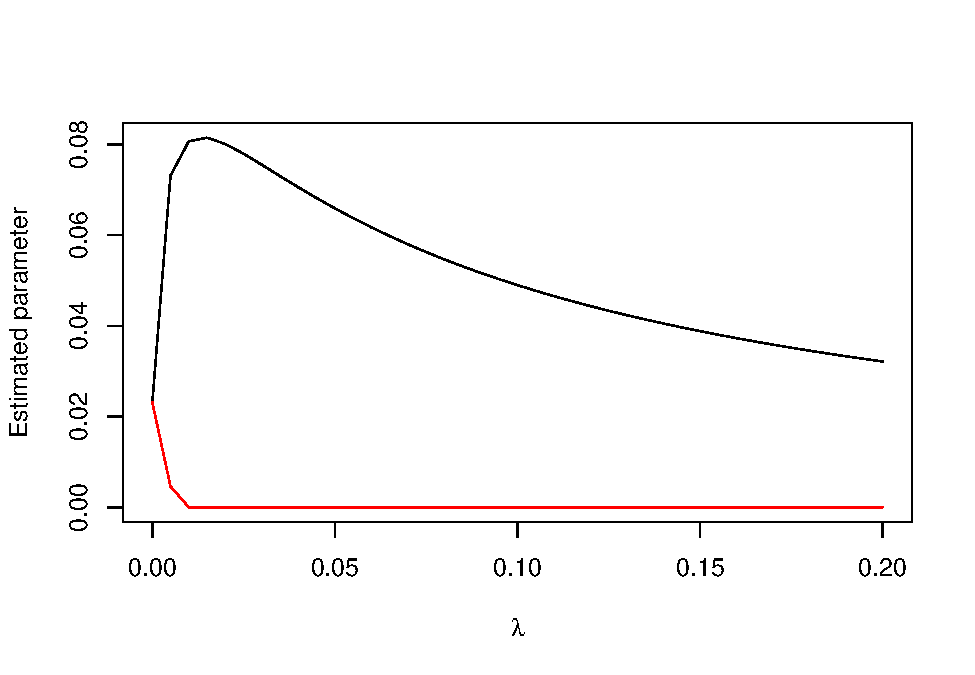
\includegraphics{AdvECTS_files/figure-latex/lasso4-1.pdf}

Let us take two values of \(\lambda\) and see the associated estimated parameters in the context of lasso regressions:

\begin{Shaded}
\begin{Highlighting}[]
\NormalTok{i }\OtherTok{\textless{}{-}} \DecValTok{20}\NormalTok{; j }\OtherTok{\textless{}{-}} \DecValTok{40}
\FunctionTok{cbind}\NormalTok{(result.lasso}\SpecialCharTok{$}\NormalTok{lambda[i],result.lasso}\SpecialCharTok{$}\NormalTok{lambda[j])}
\end{Highlighting}
\end{Shaded}

\begin{verbatim}
##       [,1]  [,2]
## [1,] 0.105 0.005
\end{verbatim}

\begin{Shaded}
\begin{Highlighting}[]
\FunctionTok{cbind}\NormalTok{(}\FunctionTok{coef}\NormalTok{(result.lasso)[,i],}\FunctionTok{coef}\NormalTok{(result.lasso)[,j])}
\end{Highlighting}
\end{Shaded}

\begin{verbatim}
##                             [,1]          [,2]
## (Intercept)           3.24385583  6.4716266208
## delinq_2yrs           0.06308870  0.0689352682
## annual_inc            0.00000000  0.0045956535
## annual_inc2           0.00000000  0.0000000000
## log_annual_inc        0.00000000 -0.0361238200
## dti                   0.00000000  0.0224224582
## installment           0.14767959  8.2287289816
## verification_status   0.00000000 -0.0009750047
## funded_amnt           0.00000000 -7.3091694210
## funded_amnt2          0.00000000 -0.4711846250
## log_funded_amnt       0.00000000 -0.2460932367
## pub_rec               0.03390816  0.0599725219
## emp_length_10         0.00000000 -0.0192494122
## owner                 0.00000000 -0.0244459908
## renter               -0.03882640 -0.0624308746
## pub_rec_bankruptcies  0.00000000  0.0000000000
## revol_util            0.00000000  0.0000000000
## revol_bal             0.00000000  0.0024022685
\end{verbatim}

\begin{Shaded}
\begin{Highlighting}[]
\CommentTok{\# Compute values of y predicted by the model, for all lambdas:}
\NormalTok{pred1 }\OtherTok{\textless{}{-}} \FunctionTok{predict}\NormalTok{(result.lasso,}\FunctionTok{as.matrix}\NormalTok{(x))}
\CommentTok{\# Compute values of y predicted by the model, for a specific value:}
\NormalTok{pred2 }\OtherTok{\textless{}{-}} \FunctionTok{predict}\NormalTok{(result.lasso,}\FunctionTok{as.matrix}\NormalTok{(x),}\AttributeTok{s=}\FloatTok{0.085}\NormalTok{)}
\end{Highlighting}
\end{Shaded}

The \texttt{glmnet} package (see \href{https://glmnet.stanford.edu/articles/glmnet.html}{Hastie et al.~(2021)}) also offers tools to implement cross-validation:

\begin{Shaded}
\begin{Highlighting}[]
\CommentTok{\# cross validation:}
\NormalTok{cvglmnet }\OtherTok{\textless{}{-}} \FunctionTok{cv.glmnet}\NormalTok{(}\FunctionTok{as.matrix}\NormalTok{(x),y)}
\FunctionTok{plot}\NormalTok{(cvglmnet)}
\end{Highlighting}
\end{Shaded}

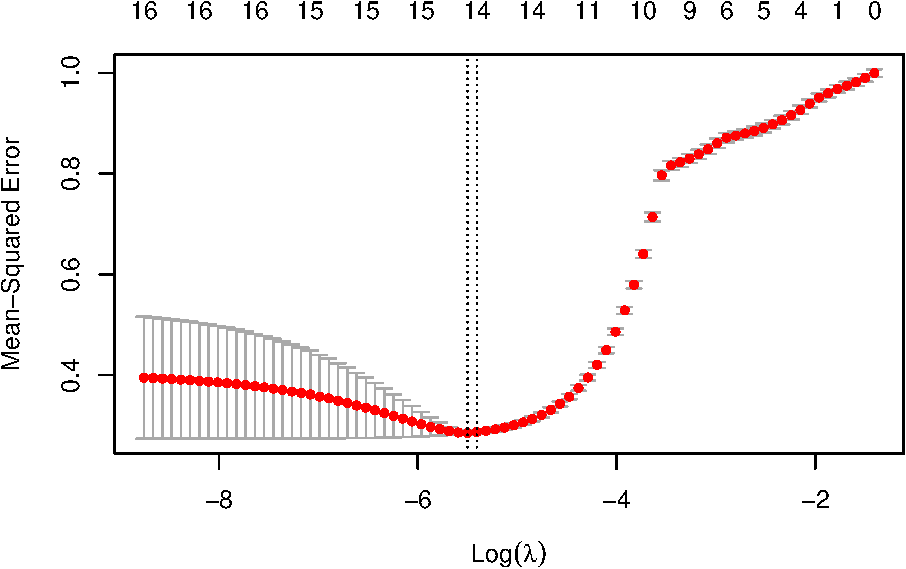
\includegraphics{AdvECTS_files/figure-latex/lasso6-1.pdf}

\begin{Shaded}
\begin{Highlighting}[]
\NormalTok{cvglmnet}\SpecialCharTok{$}\NormalTok{lambda.min }\CommentTok{\# value of lambda.min, that is the value of lambda that gives minimum mean cross{-}validated error}
\end{Highlighting}
\end{Shaded}

\begin{verbatim}
## [1] 0.004091039
\end{verbatim}

\begin{Shaded}
\begin{Highlighting}[]
\NormalTok{cvglmnet}\SpecialCharTok{$}\NormalTok{lambda}\FloatTok{.1}\NormalTok{se }\CommentTok{\# largest value of lambda that is such that the sample cost is within the +1/{-}1 standard{-}deviation band stemming from the cv procedure}
\end{Highlighting}
\end{Shaded}

\begin{verbatim}
## [1] 0.004927671
\end{verbatim}

\begin{Shaded}
\begin{Highlighting}[]
\FunctionTok{coef}\NormalTok{(cvglmnet, }\AttributeTok{s =} \StringTok{"lambda.min"}\NormalTok{) }\CommentTok{\# associated parameters}
\end{Highlighting}
\end{Shaded}

\begin{verbatim}
## 18 x 1 sparse Matrix of class "dgCMatrix"
##                                s1
## (Intercept)           6.583140504
## delinq_2yrs           0.066258597
## annual_inc            0.006054923
## annual_inc2           .          
## log_annual_inc       -0.037951509
## dti                   0.020652724
## installment           8.518960621
## verification_status  -0.002894435
## funded_amnt          -7.560852965
## funded_amnt2         -0.504192252
## log_funded_amnt      -0.253756726
## pub_rec               0.058043332
## emp_length_10        -0.018946660
## owner                -0.024841917
## renter               -0.060398310
## pub_rec_bankruptcies  .          
## revol_util            .          
## revol_bal             0.003093752
\end{verbatim}

\begin{Shaded}
\begin{Highlighting}[]
\FunctionTok{predict}\NormalTok{(cvglmnet, }\AttributeTok{newx =} \FunctionTok{as.matrix}\NormalTok{(x)[}\DecValTok{1}\SpecialCharTok{:}\DecValTok{5}\NormalTok{,], }\AttributeTok{s =} \StringTok{"lambda.min"}\NormalTok{) }\CommentTok{\# predicted values of y for specific values of x}
\end{Highlighting}
\end{Shaded}

\begin{verbatim}
##       lambda.min
## 21529   3.807030
## 21547   3.416528
## 21579   4.026621
## 21583   3.255096
## 21608   3.340412
\end{verbatim}

\hypertarget{append}{%
\chapter{Appendix}\label{append}}

\hypertarget{statistical-tables}{%
\section{Statistical Tables}\label{statistical-tables}}

\begin{table}

\caption{\label{tab:Normal}Quantiles of the $\mathcal{N}(0,1)$ distribution. If $a$ and $b$ are respectively the row and column number; then the corresponding cell gives $\mathbb{P}(0<X\le a+b)$, where $X \sim \mathcal{N}(0,1)$.}
\centering
\begin{tabular}[t]{l|r|r|r|r|r|r|r|r|r|r}
\hline
  & 0 & 0.01 & 0.02 & 0.03 & 0.04 & 0.05 & 0.06 & 0.07 & 0.08 & 0.09\\
\hline
0 & 0.5000 & 0.6179 & 0.7257 & 0.8159 & 0.8849 & 0.9332 & 0.9641 & 0.9821 & 0.9918 & 0.9965\\
\hline
0.1 & 0.5040 & 0.6217 & 0.7291 & 0.8186 & 0.8869 & 0.9345 & 0.9649 & 0.9826 & 0.9920 & 0.9966\\
\hline
0.2 & 0.5080 & 0.6255 & 0.7324 & 0.8212 & 0.8888 & 0.9357 & 0.9656 & 0.9830 & 0.9922 & 0.9967\\
\hline
0.3 & 0.5120 & 0.6293 & 0.7357 & 0.8238 & 0.8907 & 0.9370 & 0.9664 & 0.9834 & 0.9925 & 0.9968\\
\hline
0.4 & 0.5160 & 0.6331 & 0.7389 & 0.8264 & 0.8925 & 0.9382 & 0.9671 & 0.9838 & 0.9927 & 0.9969\\
\hline
0.5 & 0.5199 & 0.6368 & 0.7422 & 0.8289 & 0.8944 & 0.9394 & 0.9678 & 0.9842 & 0.9929 & 0.9970\\
\hline
0.6 & 0.5239 & 0.6406 & 0.7454 & 0.8315 & 0.8962 & 0.9406 & 0.9686 & 0.9846 & 0.9931 & 0.9971\\
\hline
0.7 & 0.5279 & 0.6443 & 0.7486 & 0.8340 & 0.8980 & 0.9418 & 0.9693 & 0.9850 & 0.9932 & 0.9972\\
\hline
0.8 & 0.5319 & 0.6480 & 0.7517 & 0.8365 & 0.8997 & 0.9429 & 0.9699 & 0.9854 & 0.9934 & 0.9973\\
\hline
0.9 & 0.5359 & 0.6517 & 0.7549 & 0.8389 & 0.9015 & 0.9441 & 0.9706 & 0.9857 & 0.9936 & 0.9974\\
\hline
1 & 0.5398 & 0.6554 & 0.7580 & 0.8413 & 0.9032 & 0.9452 & 0.9713 & 0.9861 & 0.9938 & 0.9974\\
\hline
1.1 & 0.5438 & 0.6591 & 0.7611 & 0.8438 & 0.9049 & 0.9463 & 0.9719 & 0.9864 & 0.9940 & 0.9975\\
\hline
1.2 & 0.5478 & 0.6628 & 0.7642 & 0.8461 & 0.9066 & 0.9474 & 0.9726 & 0.9868 & 0.9941 & 0.9976\\
\hline
1.3 & 0.5517 & 0.6664 & 0.7673 & 0.8485 & 0.9082 & 0.9484 & 0.9732 & 0.9871 & 0.9943 & 0.9977\\
\hline
1.4 & 0.5557 & 0.6700 & 0.7704 & 0.8508 & 0.9099 & 0.9495 & 0.9738 & 0.9875 & 0.9945 & 0.9977\\
\hline
1.5 & 0.5596 & 0.6736 & 0.7734 & 0.8531 & 0.9115 & 0.9505 & 0.9744 & 0.9878 & 0.9946 & 0.9978\\
\hline
1.6 & 0.5636 & 0.6772 & 0.7764 & 0.8554 & 0.9131 & 0.9515 & 0.9750 & 0.9881 & 0.9948 & 0.9979\\
\hline
1.7 & 0.5675 & 0.6808 & 0.7794 & 0.8577 & 0.9147 & 0.9525 & 0.9756 & 0.9884 & 0.9949 & 0.9979\\
\hline
1.8 & 0.5714 & 0.6844 & 0.7823 & 0.8599 & 0.9162 & 0.9535 & 0.9761 & 0.9887 & 0.9951 & 0.9980\\
\hline
1.9 & 0.5753 & 0.6879 & 0.7852 & 0.8621 & 0.9177 & 0.9545 & 0.9767 & 0.9890 & 0.9952 & 0.9981\\
\hline
2 & 0.5793 & 0.6915 & 0.7881 & 0.8643 & 0.9192 & 0.9554 & 0.9772 & 0.9893 & 0.9953 & 0.9981\\
\hline
2.1 & 0.5832 & 0.6950 & 0.7910 & 0.8665 & 0.9207 & 0.9564 & 0.9778 & 0.9896 & 0.9955 & 0.9982\\
\hline
2.2 & 0.5871 & 0.6985 & 0.7939 & 0.8686 & 0.9222 & 0.9573 & 0.9783 & 0.9898 & 0.9956 & 0.9982\\
\hline
2.3 & 0.5910 & 0.7019 & 0.7967 & 0.8708 & 0.9236 & 0.9582 & 0.9788 & 0.9901 & 0.9957 & 0.9983\\
\hline
2.4 & 0.5948 & 0.7054 & 0.7995 & 0.8729 & 0.9251 & 0.9591 & 0.9793 & 0.9904 & 0.9959 & 0.9984\\
\hline
2.5 & 0.5987 & 0.7088 & 0.8023 & 0.8749 & 0.9265 & 0.9599 & 0.9798 & 0.9906 & 0.9960 & 0.9984\\
\hline
2.6 & 0.6026 & 0.7123 & 0.8051 & 0.8770 & 0.9279 & 0.9608 & 0.9803 & 0.9909 & 0.9961 & 0.9985\\
\hline
2.7 & 0.6064 & 0.7157 & 0.8078 & 0.8790 & 0.9292 & 0.9616 & 0.9808 & 0.9911 & 0.9962 & 0.9985\\
\hline
2.8 & 0.6103 & 0.7190 & 0.8106 & 0.8810 & 0.9306 & 0.9625 & 0.9812 & 0.9913 & 0.9963 & 0.9986\\
\hline
2.9 & 0.6141 & 0.7224 & 0.8133 & 0.8830 & 0.9319 & 0.9633 & 0.9817 & 0.9916 & 0.9964 & 0.9986\\
\hline
\end{tabular}
\end{table}

\begin{table}

\caption{\label{tab:Student}Quantiles of the Student-$t$ distribution. The rows correspond to different degrees of freedom ($\nu$, say); the columns correspond to different probabilities ($z$, say). The cell gives $q$ that is s.t. $\mathbb{P}(-q<X<q)=z$, with $X \sim t(\nu)$.}
\centering
\begin{tabular}[t]{l|r|r|r|r|r|r|r|r}
\hline
  & 0.05 & 0.1 & 0.75 & 0.9 & 0.95 & 0.975 & 0.99 & 0.999\\
\hline
1 & 0.079 & 0.158 & 2.414 & 6.314 & 12.706 & 25.452 & 63.657 & 636.619\\
\hline
2 & 0.071 & 0.142 & 1.604 & 2.920 & 4.303 & 6.205 & 9.925 & 31.599\\
\hline
3 & 0.068 & 0.137 & 1.423 & 2.353 & 3.182 & 4.177 & 5.841 & 12.924\\
\hline
4 & 0.067 & 0.134 & 1.344 & 2.132 & 2.776 & 3.495 & 4.604 & 8.610\\
\hline
5 & 0.066 & 0.132 & 1.301 & 2.015 & 2.571 & 3.163 & 4.032 & 6.869\\
\hline
6 & 0.065 & 0.131 & 1.273 & 1.943 & 2.447 & 2.969 & 3.707 & 5.959\\
\hline
7 & 0.065 & 0.130 & 1.254 & 1.895 & 2.365 & 2.841 & 3.499 & 5.408\\
\hline
8 & 0.065 & 0.130 & 1.240 & 1.860 & 2.306 & 2.752 & 3.355 & 5.041\\
\hline
9 & 0.064 & 0.129 & 1.230 & 1.833 & 2.262 & 2.685 & 3.250 & 4.781\\
\hline
10 & 0.064 & 0.129 & 1.221 & 1.812 & 2.228 & 2.634 & 3.169 & 4.587\\
\hline
20 & 0.063 & 0.127 & 1.185 & 1.725 & 2.086 & 2.423 & 2.845 & 3.850\\
\hline
30 & 0.063 & 0.127 & 1.173 & 1.697 & 2.042 & 2.360 & 2.750 & 3.646\\
\hline
40 & 0.063 & 0.126 & 1.167 & 1.684 & 2.021 & 2.329 & 2.704 & 3.551\\
\hline
50 & 0.063 & 0.126 & 1.164 & 1.676 & 2.009 & 2.311 & 2.678 & 3.496\\
\hline
60 & 0.063 & 0.126 & 1.162 & 1.671 & 2.000 & 2.299 & 2.660 & 3.460\\
\hline
70 & 0.063 & 0.126 & 1.160 & 1.667 & 1.994 & 2.291 & 2.648 & 3.435\\
\hline
80 & 0.063 & 0.126 & 1.159 & 1.664 & 1.990 & 2.284 & 2.639 & 3.416\\
\hline
90 & 0.063 & 0.126 & 1.158 & 1.662 & 1.987 & 2.280 & 2.632 & 3.402\\
\hline
100 & 0.063 & 0.126 & 1.157 & 1.660 & 1.984 & 2.276 & 2.626 & 3.390\\
\hline
200 & 0.063 & 0.126 & 1.154 & 1.653 & 1.972 & 2.258 & 2.601 & 3.340\\
\hline
500 & 0.063 & 0.126 & 1.152 & 1.648 & 1.965 & 2.248 & 2.586 & 3.310\\
\hline
\end{tabular}
\end{table}

\begin{table}

\caption{\label{tab:Chi2}Quantiles of the $\chi^2$ distribution. The rows correspond to different degrees of freedom; the columns correspond to different probabilities.}
\centering
\begin{tabular}[t]{l|r|r|r|r|r|r|r|r}
\hline
  & 0.05 & 0.1 & 0.75 & 0.9 & 0.95 & 0.975 & 0.99 & 0.999\\
\hline
1 & 0.004 & 0.016 & 1.323 & 2.706 & 3.841 & 5.024 & 6.635 & 10.828\\
\hline
2 & 0.103 & 0.211 & 2.773 & 4.605 & 5.991 & 7.378 & 9.210 & 13.816\\
\hline
3 & 0.352 & 0.584 & 4.108 & 6.251 & 7.815 & 9.348 & 11.345 & 16.266\\
\hline
4 & 0.711 & 1.064 & 5.385 & 7.779 & 9.488 & 11.143 & 13.277 & 18.467\\
\hline
5 & 1.145 & 1.610 & 6.626 & 9.236 & 11.070 & 12.833 & 15.086 & 20.515\\
\hline
6 & 1.635 & 2.204 & 7.841 & 10.645 & 12.592 & 14.449 & 16.812 & 22.458\\
\hline
7 & 2.167 & 2.833 & 9.037 & 12.017 & 14.067 & 16.013 & 18.475 & 24.322\\
\hline
8 & 2.733 & 3.490 & 10.219 & 13.362 & 15.507 & 17.535 & 20.090 & 26.124\\
\hline
9 & 3.325 & 4.168 & 11.389 & 14.684 & 16.919 & 19.023 & 21.666 & 27.877\\
\hline
10 & 3.940 & 4.865 & 12.549 & 15.987 & 18.307 & 20.483 & 23.209 & 29.588\\
\hline
20 & 10.851 & 12.443 & 23.828 & 28.412 & 31.410 & 34.170 & 37.566 & 45.315\\
\hline
30 & 18.493 & 20.599 & 34.800 & 40.256 & 43.773 & 46.979 & 50.892 & 59.703\\
\hline
40 & 26.509 & 29.051 & 45.616 & 51.805 & 55.758 & 59.342 & 63.691 & 73.402\\
\hline
50 & 34.764 & 37.689 & 56.334 & 63.167 & 67.505 & 71.420 & 76.154 & 86.661\\
\hline
60 & 43.188 & 46.459 & 66.981 & 74.397 & 79.082 & 83.298 & 88.379 & 99.607\\
\hline
70 & 51.739 & 55.329 & 77.577 & 85.527 & 90.531 & 95.023 & 100.425 & 112.317\\
\hline
80 & 60.391 & 64.278 & 88.130 & 96.578 & 101.879 & 106.629 & 112.329 & 124.839\\
\hline
90 & 69.126 & 73.291 & 98.650 & 107.565 & 113.145 & 118.136 & 124.116 & 137.208\\
\hline
100 & 77.929 & 82.358 & 109.141 & 118.498 & 124.342 & 129.561 & 135.807 & 149.449\\
\hline
200 & 168.279 & 174.835 & 213.102 & 226.021 & 233.994 & 241.058 & 249.445 & 267.541\\
\hline
500 & 449.147 & 459.926 & 520.950 & 540.930 & 553.127 & 563.852 & 576.493 & 603.446\\
\hline
\end{tabular}
\end{table}

\begin{table}

\caption{\label{tab:Fstat}Quantiles of the $\mathcal{F}$ distribution. The columns and rows correspond to different degrees of freedom (resp. $n_1$ and $n_2$). The different panels correspond to different probabilities ($\alpha$) The corresponding cell gives $z$ that is s.t. $\mathbb{P}(X \le z)=\alpha$, with $X \sim \mathcal{F}(n_1,n_2)$.}
\centering
\begin{tabular}[t]{l|r|r|r|r|r|r|r|r|r|r}
\hline
  & 1 & 2 & 3 & 4 & 5 & 6 & 7 & 8 & 9 & 10\\
\hline
alpha = 0.9 &  &  &  &  &  &  &  &  &  & \\
\hline
5 & 4.060 & 3.780 & 3.619 & 3.520 & 3.453 & 3.405 & 3.368 & 3.339 & 3.316 & 3.297\\
\hline
10 & 3.285 & 2.924 & 2.728 & 2.605 & 2.522 & 2.461 & 2.414 & 2.377 & 2.347 & 2.323\\
\hline
15 & 3.073 & 2.695 & 2.490 & 2.361 & 2.273 & 2.208 & 2.158 & 2.119 & 2.086 & 2.059\\
\hline
20 & 2.975 & 2.589 & 2.380 & 2.249 & 2.158 & 2.091 & 2.040 & 1.999 & 1.965 & 1.937\\
\hline
50 & 2.809 & 2.412 & 2.197 & 2.061 & 1.966 & 1.895 & 1.840 & 1.796 & 1.760 & 1.729\\
\hline
100 & 2.756 & 2.356 & 2.139 & 2.002 & 1.906 & 1.834 & 1.778 & 1.732 & 1.695 & 1.663\\
\hline
500 & 2.716 & 2.313 & 2.095 & 1.956 & 1.859 & 1.786 & 1.729 & 1.683 & 1.644 & 1.612\\
\hline
alpha = 0.95 &  &  &  &  &  &  &  &  &  & \\
\hline
5 & 6.608 & 5.786 & 5.409 & 5.192 & 5.050 & 4.950 & 4.876 & 4.818 & 4.772 & 4.735\\
\hline
10 & 4.965 & 4.103 & 3.708 & 3.478 & 3.326 & 3.217 & 3.135 & 3.072 & 3.020 & 2.978\\
\hline
15 & 4.543 & 3.682 & 3.287 & 3.056 & 2.901 & 2.790 & 2.707 & 2.641 & 2.588 & 2.544\\
\hline
20 & 4.351 & 3.493 & 3.098 & 2.866 & 2.711 & 2.599 & 2.514 & 2.447 & 2.393 & 2.348\\
\hline
50 & 4.034 & 3.183 & 2.790 & 2.557 & 2.400 & 2.286 & 2.199 & 2.130 & 2.073 & 2.026\\
\hline
100 & 3.936 & 3.087 & 2.696 & 2.463 & 2.305 & 2.191 & 2.103 & 2.032 & 1.975 & 1.927\\
\hline
500 & 3.860 & 3.014 & 2.623 & 2.390 & 2.232 & 2.117 & 2.028 & 1.957 & 1.899 & 1.850\\
\hline
alpha = 0.99 &  &  &  &  &  &  &  &  &  & \\
\hline
5 & 16.258 & 13.274 & 12.060 & 11.392 & 10.967 & 10.672 & 10.456 & 10.289 & 10.158 & 10.051\\
\hline
10 & 10.044 & 7.559 & 6.552 & 5.994 & 5.636 & 5.386 & 5.200 & 5.057 & 4.942 & 4.849\\
\hline
15 & 8.683 & 6.359 & 5.417 & 4.893 & 4.556 & 4.318 & 4.142 & 4.004 & 3.895 & 3.805\\
\hline
20 & 8.096 & 5.849 & 4.938 & 4.431 & 4.103 & 3.871 & 3.699 & 3.564 & 3.457 & 3.368\\
\hline
50 & 7.171 & 5.057 & 4.199 & 3.720 & 3.408 & 3.186 & 3.020 & 2.890 & 2.785 & 2.698\\
\hline
100 & 6.895 & 4.824 & 3.984 & 3.513 & 3.206 & 2.988 & 2.823 & 2.694 & 2.590 & 2.503\\
\hline
500 & 6.686 & 4.648 & 3.821 & 3.357 & 3.054 & 2.838 & 2.675 & 2.547 & 2.443 & 2.356\\
\hline
\end{tabular}
\end{table}

\hypertarget{variousResults}{%
\section{Statistics: definitions and results}\label{variousResults}}

\begin{definition}[Partial correlation]
\protect\hypertarget{def:partialcorrel}{}\label{def:partialcorrel}The \textbf{partial correlation} between \(y\) and \(z\), controlling for some variables \(\mathbf{X}\) is the sample correlation between \(y^*\) and \(z^*\), where the latter two variables are the residuals in regressions of \(y\) on \(\mathbf{X}\) and of \(z\) on \(\mathbf{X}\), respectively.

This correlation is denoted by \(r_{yz}^\mathbf{X}\). By definition, we have:
\begin{equation}
r_{yz}^\mathbf{X} = \frac{\mathbf{z^*}'\mathbf{y^*}}{\sqrt{(\mathbf{z^*}'\mathbf{z^*})(\mathbf{y^*}'\mathbf{y^*})}}.\label{eq:pc}
\end{equation}
\end{definition}

\begin{definition}[Skewness and kurtosis]
\protect\hypertarget{def:skewnesskurtosis}{}\label{def:skewnesskurtosis}

Let \(Y\) be a random variable whose fourth moment exists. The expectation of \(Y\) is denoted by \(\mu\).

\begin{itemize}
\tightlist
\item
  The \color{blue}{skewness} of \(Y\) is given by:
  \[
  \frac{\mathbb{E}[(Y-\mu)^3]}{\{\mathbb{E}[(Y-\mu)^2]\}^{3/2}}.
  \]
\item
  The \color{blue}{kurtosis} of \(Y\) is given by:
  \[
  \frac{\mathbb{E}[(Y-\mu)^4]}{\{\mathbb{E}[(Y-\mu)^2]\}^{2}}.
  \]
\end{itemize}

\end{definition}

\begin{definition}[Eigenvalues]
\protect\hypertarget{def:determinant}{}\label{def:determinant}The eigenvalues of of a matrix \(M\) are the numbers \(\lambda\) for which:
\[
|M - \lambda I| = 0,
\]
where \(| \bullet |\) is the determinant operator.
\end{definition}

\begin{proposition}[Properties of the determinant]
\protect\hypertarget{prp:determinant}{}\label{prp:determinant}

We have:

\begin{itemize}
\tightlist
\item
  \(|MN|=|M|\times|N|\).
\item
  \(|M^{-1}|=|M|^{-1}\).
\item
  If \(M\) admits the diagonal representation \(M=TDT^{-1}\), where \(D\) is a diagonal matrix whose diagonal entries are \(\{\lambda_i\}_{i=1,\dots,n}\), then:
  \[
  |M - \lambda I |=\prod_{i=1}^n (\lambda_i - \lambda).
  \]
\end{itemize}

\end{proposition}

\begin{definition}[Moore-Penrose inverse]
\protect\hypertarget{def:MoorPenrose}{}\label{def:MoorPenrose}

If \(M \in \mathbb{R}^{m \times n}\), then its Moore-Penrose pseudo inverse (exists and) is the unique matrix \(M^* \in \mathbb{R}^{n \times m}\) that satisfies:

\begin{enumerate}
\def\labelenumi{\roman{enumi}.}
\tightlist
\item
  \(M M^* M = M\)
\item
  \(M^* M M^* = M^*\)
\item
  \((M M^*)'=M M^*\)
  .iv \((M^* M)'=M^* M\).
\end{enumerate}

\end{definition}

\begin{proposition}[Properties of the Moore-Penrose inverse]
\protect\hypertarget{prp:MoorPenrose}{}\label{prp:MoorPenrose}

\begin{itemize}
\tightlist
\item
  If \(M\) is invertible then \(M^* = M^{-1}\).
\item
  The pseudo-inverse of a zero matrix is its transpose.
  *

  \item*

  The pseudo-inverse of the pseudo-inverse is the original matrix.
\end{itemize}

\end{proposition}

\begin{definition}[F distribution]
\protect\hypertarget{def:fstatistics}{}\label{def:fstatistics}Consider \(n=n_1+n_2\) i.i.d. \(\mathcal{N}(0,1)\) r.v. \(X_i\). If the r.v. \(F\) is defined by:
\[
F = \frac{\sum_{i=1}^{n_1} X_i^2}{\sum_{j=n_1+1}^{n_1+n_2} X_j^2}\frac{n_2}{n_1}
\]
then \(F \sim \mathcal{F}(n_1,n_2)\). (See Table \ref{tab:Fstat} for quantiles.)
\end{definition}

\begin{definition}[Student-t distribution]
\protect\hypertarget{def:tStudent}{}\label{def:tStudent}\(Z\) follows a Student-t (or \(t\)) distribution with \(\nu\) degrees of freedom (d.f.) if:
\[
Z = X_0 \bigg/ \sqrt{\frac{\sum_{i=1}^{\nu}X_i^2}{\nu}}, \quad X_i \sim i.i.d. \mathcal{N}(0,1).
\]
We have \(\mathbb{E}(Z)=0\), and \(\mathbb{V}ar(Z)=\frac{\nu}{\nu-2}\) if \(\nu>2\). (See Table \ref{tab:Student} for quantiles.)
\end{definition}

\begin{definition}[Chi-square distribution]
\protect\hypertarget{def:chi2}{}\label{def:chi2}\(Z\) follows a \(\chi^2\) distribution with \(\nu\) d.f. if \(Z = \sum_{i=1}^{\nu}X_i^2\) where \(X_i \sim i.i.d. \mathcal{N}(0,1)\).
We have \(\mathbb{E}(Z)=\nu\). (See Table \ref{tab:Chi2} for quantiles.)
\end{definition}

\begin{definition}[Idempotent matrix]
\protect\hypertarget{def:idempotent}{}\label{def:idempotent}Matrix \(M\) is idempotent if \(M^2=M\).

If \(M\) is a symmetric idempotent matrix, then \(M'M=M\).
\end{definition}

\begin{proposition}[Roots of an idempotent matrix]
\protect\hypertarget{prp:rootsidempotent}{}\label{prp:rootsidempotent}The eigenvalues of an idempotent matrix are either 1 or 0.
\end{proposition}

\begin{proof}
If \(\lambda\) is an eigenvalue of an idempotent matrix \(M\) then \(\exists x \ne 0\) s.t. \(Mx=\lambda x\). Hence \(M^2x=\lambda M x \Rightarrow (1-\lambda)Mx=0\). Either all element of \(Mx\) are zero, in which case \(\lambda=0\) or at least one element of \(Mx\) is nonzero, in which case \(\lambda=1\).
\end{proof}

\begin{proposition}[Idempotent matrix and chi-square distribution]
\protect\hypertarget{prp:chi2idempotent}{}\label{prp:chi2idempotent}The rank of a symmetric idempotent matrix is equal to its trace.
\end{proposition}

\begin{proof}
The result follows from Prop. \ref{prp:rootsidempotent}, combined with the fact that the rank of a symmetric matrix is equal to the number of its nonzero eigenvalues.
\end{proof}

\begin{proposition}[Constrained least squares]
\protect\hypertarget{prp:constrainedLS}{}\label{prp:constrainedLS}The solution of the following optimisation problem:
\begin{eqnarray*}
\underset{\boldsymbol\beta}{\min} && || \mathbf{y} - \mathbf{X}\boldsymbol\beta ||^2 \\
&& \mbox{subject to } \mathbf{R}\boldsymbol\beta = \mathbf{q}
\end{eqnarray*}
is given by:
\[
\boxed{\boldsymbol\beta^r = \boldsymbol\beta_0 - (\mathbf{X}'\mathbf{X})^{-1} \mathbf{R}'\{\mathbf{R}(\mathbf{X}'\mathbf{X})^{-1}\mathbf{R}'\}^{-1}(\mathbf{R}\boldsymbol\beta_0 - \mathbf{q}),}
\]
where \(\boldsymbol\beta_0=(\mathbf{X}'\mathbf{X})^{-1}\mathbf{X}'\mathbf{y}\).
\end{proposition}

\begin{proof}
See for instance \href{http://jackman.stanford.edu/classes/350B/07/ftestforWeb.pdf}{Jackman, 2007}.
\end{proof}

\begin{proposition}[Chebychev's inequality]
\protect\hypertarget{prp:chebychev}{}\label{prp:chebychev}If \(\mathbb{E}(|X|^r)\) is finite for some \(r>0\) then:
\[
\forall \varepsilon > 0, \quad \mathbb{P}(|X - c|>\varepsilon) \le \frac{\mathbb{E}[|X - c|^r]}{\varepsilon^r}.
\]
In particular, for \(r=2\):
\[
\forall \varepsilon > 0, \quad \mathbb{P}(|X - c|>\varepsilon) \le \frac{\mathbb{E}[(X - c)^2]}{\varepsilon^2}.
\]
\end{proposition}

\begin{proof}
Remark that \(\varepsilon^r \mathbb{I}_{\{|X| \ge \varepsilon\}} \le |X|^r\) and take the expectation of both sides.
\end{proof}

\begin{definition}[Convergence in probability]
\protect\hypertarget{def:convergenceproba}{}\label{def:convergenceproba}The random variable sequence \(x_n\) converges in probability to a constant \(c\) if \(\forall \varepsilon\), \(\lim_{n \rightarrow \infty} \mathbb{P}(|x_n - c|>\varepsilon) = 0\).

It is denoted as: \(\mbox{plim } x_n = c\).
\end{definition}

\begin{definition}[Convergence in the Lr norm]
\protect\hypertarget{def:convergenceLr}{}\label{def:convergenceLr}\(x_n\) converges in the \(r\)-th mean (or in the \(L^r\)-norm) towards \(x\), if \(\mathbb{E}(|x_n|^r)\) and \(\mathbb{E}(|x|^r)\) exist and if
\[
\lim_{n \rightarrow \infty} \mathbb{E}(|x_n - x|^r) = 0.
\]
It is denoted as: \(x_n \overset{L^r}{\rightarrow} c\).

For \(r=2\), this convergence is called \textbf{mean square convergence}.
\end{definition}

\begin{definition}[Almost sure convergence]
\protect\hypertarget{def:convergenceAlmost}{}\label{def:convergenceAlmost}The random variable sequence \(x_n\) converges almost surely to \(c\) if \(\mathbb{P}(\lim_{n \rightarrow \infty} x_n = c) = 1\).

It is denoted as: \(x_n \overset{a.s.}{\rightarrow} c\).
\end{definition}

\begin{definition}[Convergence in distribution]
\protect\hypertarget{def:cvgceDistri}{}\label{def:cvgceDistri}\(x_n\) is said to converge in distribution (or in law) to \(x\) if
\[
\lim_{n \rightarrow \infty} F_{x_n}(s) = F_{x}(s)
\]
for all \(s\) at which \(F_X\) --the cumulative distribution of \(X\)-- is continuous.

It is denoted as: \(x_n \overset{d}{\rightarrow} x\).
\end{definition}

\begin{proposition}[Rules for limiting distributions (Slutsky)]
\protect\hypertarget{prp:Slutsky}{}\label{prp:Slutsky}

We have:

\begin{enumerate}
\def\labelenumi{\roman{enumi}.}
\item
  \textbf{Slutsky's theorem:} If \(x_n \overset{d}{\rightarrow} x\) and \(y_n \overset{p}{\rightarrow} c\) then
  \begin{eqnarray*}
  x_n y_n &\overset{d}{\rightarrow}& x c \\
  x_n + y_n &\overset{d}{\rightarrow}& x + c \\
  x_n/y_n &\overset{d}{\rightarrow}& x / c \quad (\mbox{if }c \ne 0)
  \end{eqnarray*}
\item
  \textbf{Continuous mapping theorem:} If \(x_n \overset{d}{\rightarrow} x\) and \(g\) is a continuous function then \(g(x_n) \overset{d}{\rightarrow} g(x).\)
\end{enumerate}

\end{proposition}

\begin{proposition}[Implications of stochastic convergences]
\protect\hypertarget{prp:implicationsconv}{}\label{prp:implicationsconv}We have:
\begin{align*}
&\boxed{\overset{L^s}{\rightarrow}}& &\underset{1 \le r \le s}{\Rightarrow}& &\boxed{\overset{L^r}{\rightarrow}}&\\
&& && &\Downarrow&\\
&\boxed{\overset{a.s.}{\rightarrow}}& &\Rightarrow& &\boxed{\overset{p}{\rightarrow}}& \Rightarrow \qquad \boxed{\overset{d}{\rightarrow}}.
\end{align*}
\end{proposition}

\begin{proof}
(of the fact that \(\left(\overset{p}{\rightarrow}\right) \Rightarrow \left( \overset{d}{\rightarrow}\right)\)). Assume that \(X_n \overset{p}{\rightarrow} X\). Denoting by \(F\) and \(F_n\) the c.d.f. of \(X\) and \(X_n\), respectively:
\begin{equation}
F_n(x) = \mathbb{P}(X_n \le x,X\le x+\varepsilon) + \mathbb{P}(X_n \le x,X > x+\varepsilon) \le F(x+\varepsilon) + \mathbb{P}(|X_n - X|>\varepsilon).\label{eq:convgce1}
\end{equation}
Besides,
\[
F(x-\varepsilon) = \mathbb{P}(X \le x-\varepsilon,X_n \le x) + \mathbb{P}(X \le x-\varepsilon,X_n > x) \le F_n(x) + \mathbb{P}(|X_n - X|>\varepsilon),
\]
which implies:
\begin{equation}
F(x-\varepsilon) - \mathbb{P}(|X_n - X|>\varepsilon) \le F_n(x).\label{eq:convgce2}
\end{equation}
Eqs. \eqref{eq:convgce1} and \eqref{eq:convgce2} imply:
\[
F(x-\varepsilon) - \mathbb{P}(|X_n - X|>\varepsilon) \le F_n(x)  \le F(x+\varepsilon) + \mathbb{P}(|X_n - X|>\varepsilon).
\]
Taking limits as \(n \rightarrow \infty\) yields
\[
F(x-\varepsilon) \le \underset{n \rightarrow \infty}{\mbox{lim inf}}\; F_n(x) \le \underset{n \rightarrow \infty}{\mbox{lim sup}}\; F_n(x)  \le F(x+\varepsilon).
\]
The result is then obtained by taking limits as \(\varepsilon \rightarrow 0\) (if \(F\) is continuous at \(x\)).
\end{proof}

\begin{proposition}[Convergence in distribution to a constant]
\protect\hypertarget{prp:cvgce11}{}\label{prp:cvgce11}If \(X_n\) converges in distribution to a constant \(c\), then \(X_n\) converges in probability to \(c\).
\end{proposition}

\begin{proof}
If \(\varepsilon>0\), we have \(\mathbb{P}(X_n < c - \varepsilon) \underset{n \rightarrow \infty}{\rightarrow} 0\) i.e.~\(\mathbb{P}(X_n \ge c - \varepsilon) \underset{n \rightarrow \infty}{\rightarrow} 1\) and \(\mathbb{P}(X_n < c + \varepsilon) \underset{n \rightarrow \infty}{\rightarrow} 1\). Therefore \(\mathbb{P}(c - \varepsilon \le X_n < c + \varepsilon) \underset{n \rightarrow \infty}{\rightarrow} 1\),
which gives the result.
\end{proof}

\textbf{Example of \(plim\) but not \(L^r\) convergence}: Let \(\{x_n\}_{n \in \mathbb{N}}\) be a series of random variables defined by:
\[
x_n = n u_n,
\]
where \(u_n\) are independent random variables s.t. \(u_n \sim \mathcal{B}(1/n)\).

We have \(x_n \overset{p}{\rightarrow} 0\) but \(x_n \overset{L^r}{\nrightarrow} 0\) because \(\mathbb{E}(|X_n-0|)=\mathbb{E}(X_n)=1\).

\begin{theorem}[Cauchy criterion (non-stochastic case)]
\protect\hypertarget{thm:cauchycritstatic}{}\label{thm:cauchycritstatic}We have that \(\sum_{i=0}^{T} a_i\) converges (\(T \rightarrow \infty\)) iff, for any \(\eta > 0\), there exists an integer \(N\) such that, for all \(M\ge N\),
\[
\left|\sum_{i=N+1}^{M} a_i\right| < \eta.
\]
\end{theorem}

\begin{theorem}[Cauchy criterion (stochastic case)]
\protect\hypertarget{thm:cauchycritstochastic}{}\label{thm:cauchycritstochastic}We have that \(\sum_{i=0}^{T} \theta_i \varepsilon_{t-i}\) converges in mean square (\(T \rightarrow \infty\)) to a random variable iff, for any \(\eta > 0\), there exists an integer \(N\) such that, for all \(M\ge N\),
\[
\mathbb{E}\left[\left(\sum_{i=N+1}^{M} \theta_i \varepsilon_{t-i}\right)^2\right] < \eta.
\]
\end{theorem}

\begin{definition}[Characteristic function]
\protect\hypertarget{def:characteristic}{}\label{def:characteristic}For any real-valued random variable \(X\), the characteristic function is defined by:
\[
\phi_X: u \rightarrow \mathbb{E}[\exp(iuX)].
\]
\end{definition}

\begin{theorem}[Law of large numbers]
\protect\hypertarget{thm:LLNappendix}{}\label{thm:LLNappendix}The sample mean is a consistent estimator of the population mean.
\end{theorem}

\begin{proof}
Let's denote by \(\phi_{X_i}\) the characteristic function of a r.v. \(X_i\). If the mean of \(X_i\) is \(\mu\) then the Talyor expansion of the characteristic function is:
\[
\phi_{X_i}(u) = \mathbb{E}(\exp(iuX)) = 1 + iu\mu + o(u).
\]
The properties of the characteristic function (see Def. \ref{def:characteristic}) imply that:
\[
\phi_{\frac{1}{n}(X_1+\dots+X_n)}(u) = \prod_{i=1}^{n} \left(1 + i\frac{u}{n}\mu + o\left(\frac{u}{n}\right) \right) \rightarrow e^{iu\mu}.
\]
The facts that (a) \(e^{iu\mu}\) is the characteristic function of the constant \(\mu\) and (b) that a characteristic function uniquely characterises a distribution imply that the sample mean converges in distribution to the constant \(\mu\), which further implies that it converges in probability to \(\mu\).
\end{proof}

\begin{theorem}[Lindberg-Levy Central limit theorem, CLT]
\protect\hypertarget{thm:LindbergLevyCLT}{}\label{thm:LindbergLevyCLT}If \(x_n\) is an i.i.d. sequence of random variables with mean \(\mu\) and variance \(\sigma^2\) (\(\in ]0,+\infty[\)), then:
\[
\boxed{\sqrt{n} (\bar{x}_n - \mu) \overset{d}{\rightarrow} \mathcal{N}(0,\sigma^2), \quad \mbox{where} \quad \bar{x}_n = \frac{1}{n} \sum_{i=1}^{n} x_i.}
\]
\end{theorem}

\begin{proof}
Let us introduce the r.v. \(Y_n:= \sqrt{n}(\bar{X}_n - \mu)\). We have \(\phi_{Y_n}(u) = \left[ \mathbb{E}\left( \exp(i \frac{1}{\sqrt{n}} u (X_1 - \mu)) \right) \right]^n\). We have:
\begin{eqnarray*}
\left[ \mathbb{E}\left( \exp\left(i \frac{1}{\sqrt{n}} u (X_1 - \mu)\right) \right) \right]^n &=& \left[ \mathbb{E}\left( 1 + i \frac{1}{\sqrt{n}} u (X_1 - \mu) - \frac{1}{2n} u^2 (X_1 - \mu)^2 + o(u^2) \right) \right]^n \\
&=& \left( 1 - \frac{1}{2n}u^2\sigma^2 + o(u^2)\right)^n.
\end{eqnarray*}
Therefore \(\phi_{Y_n}(u) \underset{n \rightarrow \infty}{\rightarrow} \exp \left( - \frac{1}{2}u^2\sigma^2 \right)\), which is the characteristic function of \(\mathcal{N}(0,\sigma^2)\).
\end{proof}

\begin{proposition}[Inverse of a partitioned matrix]
\protect\hypertarget{prp:inversepartitioned}{}\label{prp:inversepartitioned}We have:
\begin{eqnarray*}
&&\left[ \begin{array}{cc} \mathbf{A}_{11} & \mathbf{A}_{12} \\ \mathbf{A}_{21} & \mathbf{A}_{22} \end{array}\right]^{-1} = \\
&&\left[ \begin{array}{cc} (\mathbf{A}_{11} - \mathbf{A}_{12}\mathbf{A}_{22}^{-1}\mathbf{A}_{21})^{-1} & - \mathbf{A}_{11}^{-1}\mathbf{A}_{12}(\mathbf{A}_{22} - \mathbf{A}_{21}\mathbf{A}_{11}^{-1}\mathbf{A}_{12})^{-1} \\
-(\mathbf{A}_{22} - \mathbf{A}_{21}\mathbf{A}_{11}^{-1}\mathbf{A}_{12})^{-1}\mathbf{A}_{21}\mathbf{A}_{11}^{-1} & (\mathbf{A}_{22} - \mathbf{A}_{21}\mathbf{A}_{11}^{-1}\mathbf{A}_{12})^{-1} \end{array} \right].
\end{eqnarray*}
\end{proposition}

\begin{proposition}
\protect\hypertarget{prp:bandsindependent}{}\label{prp:bandsindependent}If \(\mathbf{A}\) is idempotent and if \(\mathbf{x}\) is Gaussian, \(\mathbf{L}\mathbf{x}\) and \(\mathbf{x}'\mathbf{A}\mathbf{x}\) are independent if \(\mathbf{L}\mathbf{A}=\mathbf{0}\).
\end{proposition}

\begin{proof}
If \(\mathbf{L}\mathbf{A}=\mathbf{0}\), then the two Gaussian vectors \(\mathbf{L}\mathbf{x}\) and \(\mathbf{A}\mathbf{x}\) are independent. This implies the independence of any function of \(\mathbf{L}\mathbf{x}\) and any function of \(\mathbf{A}\mathbf{x}\). The results then follows from the observation that \(\mathbf{x}'\mathbf{A}\mathbf{x}=(\mathbf{A}\mathbf{x})'(\mathbf{A}\mathbf{x})\), which is a function of \(\mathbf{A}\mathbf{x}\).
\end{proof}

\begin{proposition}[Inner product of a multivariate Gaussian variable]
\protect\hypertarget{prp:waldtypeproduct}{}\label{prp:waldtypeproduct}Let \(X\) be a \(n\)-dimensional multivariate Gaussian variable: \(X \sim \mathcal{N}(0,\Sigma)\). We have:
\[
X' \Sigma^{-1}X \sim \chi^2(n).
\]
\end{proposition}

\begin{proof}
Because \(\Sigma\) is a symmetrical definite positive matrix, it admits the spectral decomposition \(PDP'\) where \(P\) is an orthogonal matrix (i.e.~\(PP'=Id\)) and D is a diagonal matrix with non-negative entries. Denoting by \(\sqrt{D^{-1}}\) the diagonal matrix whose diagonal entries are the inverse of those of \(D\), it is easily checked that the covariance matrix of \(Y:=\sqrt{D^{-1}}P'X\) is \(Id\). Therefore \(Y\) is a vector of uncorrelated Gaussian variables. The properties of Gaussian variables imply that the components of \(Y\) are then also independent. Hence \(Y'Y=\sum_i Y_i^2 \sim \chi^2(n)\).

It remains to note that \(Y'Y=X'PD^{-1}P'X=X'\mathbb{V}ar(X)^{-1}X\) to conclude.
\end{proof}

\begin{theorem}[Cauchy-Schwarz inequality]
\protect\hypertarget{thm:CauchySchwarz}{}\label{thm:CauchySchwarz}We have:
\[
|\mathbb{C}ov(X,Y)| \le \sqrt{\mathbb{V}ar(X)\mathbb{V}ar(Y)}
\]
and, if \(X \ne =\) and \(Y \ne 0\), the equality holds iff \(X\) and \(Y\) are the same up to an affine transformation.
\end{theorem}

\begin{proof}
If \(\mathbb{V}ar(X)=0\), this is trivial. If this is not the case, then let's define \(Z\) as \(Z = Y - \frac{\mathbb{C}ov(X,Y)}{\mathbb{V}ar(X)}X\). It is easily seen that \(\mathbb{C}ov(X,Z)=0\). Then, the variance of \(Y=Z+\frac{\mathbb{C}ov(X,Y)}{\mathbb{V}ar(X)}X\) is equal to the sum of the variance of \(Z\) and of the variance of \(\frac{\mathbb{C}ov(X,Y)}{\mathbb{V}ar(X)}X\), that is:
\[
\mathbb{V}ar(Y) = \mathbb{V}ar(Z) + \left(\frac{\mathbb{C}ov(X,Y)}{\mathbb{V}ar(X)}\right)^2\mathbb{V}ar(X) \ge \left(\frac{\mathbb{C}ov(X,Y)}{\mathbb{V}ar(X)}\right)^2\mathbb{V}ar(X).
\]
The equality holds iff \(\mathbb{V}ar(Z)=0\), i.e.~iff \(Y = \frac{\mathbb{C}ov(X,Y)}{\mathbb{V}ar(X)}X+cst\).
\end{proof}

\begin{definition}[Matrix derivatives]
\protect\hypertarget{def:FOD}{}\label{def:FOD}Consider a fonction \(f: \mathbb{R}^K \rightarrow \mathbb{R}\). Its first-order derivative is:
\[
\frac{\partial f}{\partial \mathbf{b}}(\mathbf{b}) =
\left[\begin{array}{c}
\frac{\partial f}{\partial b_1}(\mathbf{b})\\
\vdots\\
\frac{\partial f}{\partial b_K}(\mathbf{b})
\end{array}
\right].
\]
We use the notation:
\[
\frac{\partial f}{\partial \mathbf{b}'}(\mathbf{b}) = \left(\frac{\partial f}{\partial \mathbf{b}}(\mathbf{b})\right)'.
\]
\end{definition}

\begin{proposition}
\protect\hypertarget{prp:partial}{}\label{prp:partial}

We have:

\begin{itemize}
\tightlist
\item
  If \(f(\mathbf{b}) = A' \mathbf{b}\) where \(A\) is a \(K \times 1\) vector then \(\frac{\partial f}{\partial \mathbf{b}}(\mathbf{b}) = A\).
\item
  If \(f(\mathbf{b}) = \mathbf{b}'A\mathbf{b}\) where \(A\) is a \(K \times K\) matrix, then \(\frac{\partial f}{\partial \mathbf{b}}(\mathbf{b}) = 2A\mathbf{b}\).
\end{itemize}

\end{proposition}

\begin{definition}[Asymptotic level]
\protect\hypertarget{def:asmyptlevel}{}\label{def:asmyptlevel}An asymptotic test with critical region \(\Omega_n\) has an \color{blue}{asymptotic level} equal to \(\alpha\) if:
\[
\underset{\theta \in \Theta}{\mbox{sup}} \quad \underset{n \rightarrow \infty}{\mbox{lim}} \mathbb{P}_\theta (S_n \in \Omega_n) = \alpha,
\]
where \(S_n\) is the test statistic and \(\Theta\) is such that the null hypothesis \(H_0\) is equivalent to \(\theta \in \Theta\).
\end{definition}

\begin{definition}[Asymptotically consistent test]
\protect\hypertarget{def:asmyptconsisttest}{}\label{def:asmyptconsisttest}An asymptotic test with critical region \(\Omega_n\) is consistent if:
\[
\forall \theta \in \Theta^c, \quad \mathbb{P}_\theta (S_n \in \Omega_n) \rightarrow 1,
\]
where \(S_n\) is the test statistic and \(\Theta^c\) is such that the null hypothesis \(H_0\) is equivalent to \(\theta \notin \Theta^c\).
\end{definition}

\begin{definition}[Kullback discrepancy]
\protect\hypertarget{def:Kullback}{}\label{def:Kullback}Given two p.d.f. \(f\) and \(f^*\), the Kullback discrepancy is defined by:
\[
I(f,f^*) = \mathbb{E}^* \left( \log \frac{f^*(Y)}{f(Y)} \right) = \int \log \frac{f^*(y)}{f(y)} f^*(y) dy.
\]
\end{definition}

\begin{center}\rule{0.5\linewidth}{0.5pt}\end{center}

\begin{proposition}[Properties of the Kullback discrepancy]
\protect\hypertarget{prp:Kullback}{}\label{prp:Kullback}

We have:

\begin{enumerate}
\def\labelenumi{\roman{enumi}.}
\item
  \(I(f,f^*) \ge 0\)
\item
  \(I(f,f^*) = 0\) iff \(f \equiv f^*\).
\end{enumerate}

\end{proposition}

\begin{center}\rule{0.5\linewidth}{0.5pt}\end{center}

\begin{proof}
\(x \rightarrow -\log(x)\) is a convex function. Therefore \(\mathbb{E}^*(-\log f(Y)/f^*(Y)) \ge -\log \mathbb{E}^*(f(Y)/f^*(Y)) = 0\) (proves (i)). Since \(x \rightarrow -\log(x)\) is strictly convex, equality in (i) holds if and only if \(f(Y)/f^*(Y)\) is constant (proves (ii)).
\end{proof}

\begin{center}\rule{0.5\linewidth}{0.5pt}\end{center}

\begin{proposition}[Square and absolute summability]
\protect\hypertarget{prp:absMs}{}\label{prp:absMs}We have:
\[
\underbrace{\sum_{i=0}^{\infty}|\theta_i| < + \infty}_{\mbox{Absolute summability}} \Rightarrow \underbrace{\sum_{i=0}^{\infty} \theta_i^2 < + \infty}_{\mbox{Square summability}}.
\]
\end{proposition}

\begin{center}\rule{0.5\linewidth}{0.5pt}\end{center}

\begin{proof}
See Appendix 3.A in Hamilton. Idea: Absolute summability implies that there exist \(N\) such that, for \(j>N\), \(|\theta_j| < 1\) (deduced from Cauchy criterion, Theorem \ref{thm:cauchycritstatic} and therefore \(\theta_j^2 < |\theta_j|\).
\end{proof}

\hypertarget{GaussianVar}{%
\section{Some properties of Gaussian variables}\label{GaussianVar}}

\begin{center}\rule{0.5\linewidth}{0.5pt}\end{center}

\begin{proposition}[Bayesian update in a vector of Gaussian variables]
\protect\hypertarget{prp:update}{}\label{prp:update}If
\[
\left[
\begin{array}{c}
Y_1\\
Y_2
\end{array}
\right]
\sim \mathcal{N}
\left(0,
\left[\begin{array}{cc}
\Omega_{11} & \Omega_{12}\\
\Omega_{21} & \Omega_{22}
\end{array}\right]
\right),
\]
then
\[
Y_{2}|Y_{1} \sim \mathcal{N}
\left(
\Omega_{21}\Omega_{11}^{-1}Y_{1},\Omega_{22}-\Omega_{21}\Omega_{11}^{-1}\Omega_{12}
\right).
\]
\[
Y_{1}|Y_{2} \sim \mathcal{N}
\left(
\Omega_{12}\Omega_{22}^{-1}Y_{2},\Omega_{11}-\Omega_{12}\Omega_{22}^{-1}\Omega_{21}
\right).
\]
\end{proposition}

\begin{center}\rule{0.5\linewidth}{0.5pt}\end{center}

\begin{center}\rule{0.5\linewidth}{0.5pt}\end{center}

\begin{proposition}[Truncated distributions]
\protect\hypertarget{prp:truncated}{}\label{prp:truncated}If \(X\) is a random variable distributed according to some p.d.f. \(f\), with c.d.f. \(F\), with infinite support. Then the p.d.f. of \(X|a \le X < b\) is
\[
g(x) = \frac{f(x)}{F(b)-F(a)}\mathbb{I}_{\{a \le x < b\}},
\]
for any \(a<b\).

In partiucular, for a Gaussian variable \(X \sim \mathcal{N}(\mu,\sigma^2)\), we have
\[
f(X=x|a\le X<b) = \dfrac{\dfrac{1}{\sigma}\phi\left(\dfrac{x - \mu}{\sigma}\right)}{Z}.
\]
with \(Z = \Phi(\beta)-\Phi(\alpha)\), where \(\alpha = \dfrac{a - \mu}{\sigma}\) and \(\beta = \dfrac{b - \mu}{\sigma}\).

Moreover:
\begin{eqnarray}
\mathbb{E}(X|a\le X<b) &=& \mu - \frac{\phi\left(\beta\right)-\phi\left(\alpha\right)}{Z}\sigma. \label{eq:Etrunc}
\end{eqnarray}

We also have:
\begin{eqnarray}
&& \mathbb{V}ar(X|a\le X<b) \nonumber\\
&=& \sigma^2\left[
1 -  \frac{\beta\phi\left(\beta\right)-\alpha\phi\left(\alpha\right)}{Z} -  \left(\frac{\phi\left(\beta\right)-\phi\left(\alpha\right)}{Z}\right)^2 \right] \label{eq:Vtrunc}
\end{eqnarray}

In particular, for \(b \rightarrow \infty\), we get:
\begin{equation}
\mathbb{V}ar(X|a < X) = \sigma^2\left[1 + \alpha\lambda(-\alpha) - \lambda(-\alpha)^2 \right], \label{eq:Vtrunc2}
\end{equation}
with \(\lambda(x)=\dfrac{\phi(x)}{\Phi(x)}\) is called the \textbf{inverse Mills ratio}.
\end{proposition}

\begin{center}\rule{0.5\linewidth}{0.5pt}\end{center}

Consider the case where \(a \rightarrow - \infty\) (i.e.~the conditioning set is \(X<b\)) and \(\mu=0\), \(\sigma=1\). Then Eq. \eqref{eq:Etrunc} gives \(\mathbb{E}(X|X<b) = - \lambda(b) = - \dfrac{\phi(b)}{\Phi(b)}\), where \(\lambda\) is the function computing the inverse Mills ratio.

\begin{figure}

{\centering 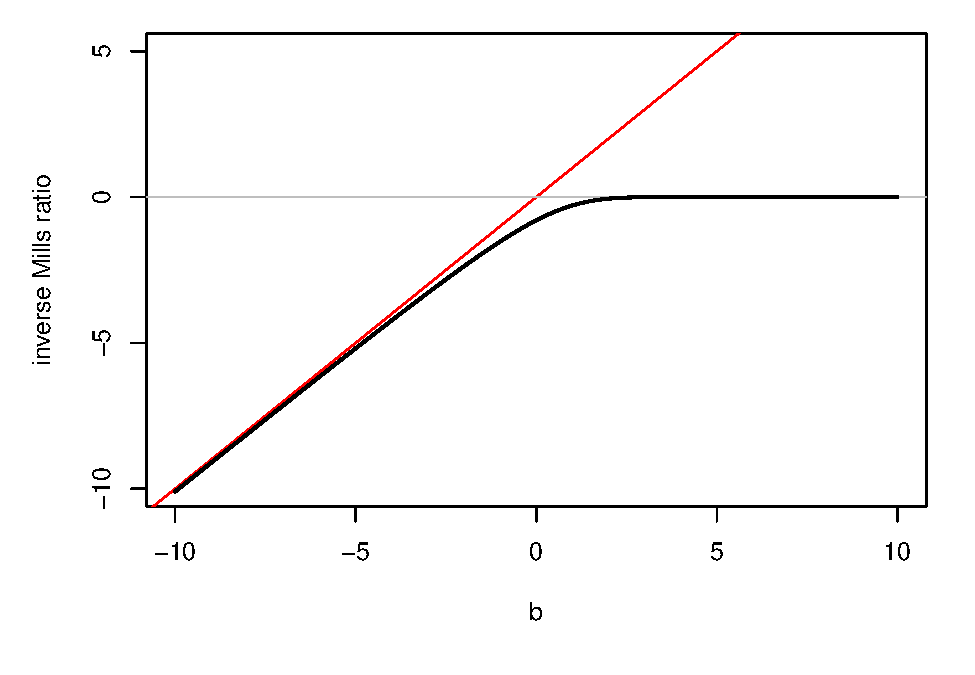
\includegraphics{AdvECTS_files/figure-latex/inverseMills-1} 

}

\caption{$\mathbb{E}(X|X<b)$ as a function of $b$ when $X\sim \mathcal{N}(0,1)$ (in black).}\label{fig:inverseMills}
\end{figure}

\begin{proposition}[p.d.f. of a multivariate Gaussian variable]
\protect\hypertarget{prp:pdfMultivarGaussian}{}\label{prp:pdfMultivarGaussian}If \(Y \sim \mathcal{N}(\mu,\Omega)\) and if \(Y\) is a \(n\)-dimensional vector, then the density function of \(Y\) is:
\[
\frac{1}{(2 \pi)^{n/2}|\Omega|^{1/2}}\exp\left[-\frac{1}{2}\left(Y-\mu\right)'\Omega^{-1}\left(Y-\mu\right)\right].
\]
\end{proposition}

\hypertarget{proofs}{%
\section{Proofs}\label{proofs}}

\hypertarget{MLEproperties}{%
\subsection{Proof of Proposition \ref{prp:MLEproperties}}\label{MLEproperties}}

\begin{proof}
Assumptions (i) and (ii) (in the set of Assumptions \ref{hyp:MLEregularity}) imply that \(\boldsymbol\theta_{MLE}\) exists (\(=\mbox{argmax}_\theta (1/n)\log \mathcal{L}(\boldsymbol\theta;\mathbf{y})\)).

\((1/n)\log \mathcal{L}(\boldsymbol\theta;\mathbf{y})\) can be interpreted as the sample mean of the r.v. \(\log f(Y_i;\boldsymbol\theta)\) that are i.i.d. Therefore \((1/n)\log \mathcal{L}(\boldsymbol\theta;\mathbf{y})\) converges to \(\mathbb{E}_{\boldsymbol\theta_0}(\log f(Y;\boldsymbol\theta))\) -- which exists (Assumption iv).

Because the latter convergence is uniform (Assumption v), the solution \(\boldsymbol\theta_{MLE}\) almost surely converges to the solution to the limit problem:
\[
\mbox{argmax}_\theta \mathbb{E}_{\boldsymbol\theta_0}(\log f(Y;\boldsymbol\theta)) = \mbox{argmax}_\theta \int_{\mathcal{Y}} \log f(y;\boldsymbol\theta)f(y;\boldsymbol\theta_0) dy.
\]

Properties of the Kullback information measure (see Prop. \ref{prp:Kullback}), together with the identifiability assumption (ii) implies that the solution to the limit problem is unique and equal to \(\boldsymbol\theta_0\).

Consider a r.v. sequence \(\boldsymbol\theta\) that converges to \(\boldsymbol\theta_0\). The Taylor expansion of the score in a neighborood of \(\boldsymbol\theta_0\) yields to:
\[
\frac{\partial \log \mathcal{L}(\boldsymbol\theta;\mathbf{y})}{\partial \boldsymbol\theta} = \frac{\partial \log \mathcal{L}(\boldsymbol\theta_0;\mathbf{y})}{\partial \boldsymbol\theta} + \frac{\partial^2 \log \mathcal{L}(\boldsymbol\theta_0;\mathbf{y})}{\partial \boldsymbol\theta \partial \boldsymbol\theta'}(\boldsymbol\theta - \boldsymbol\theta_0) + o_p(\boldsymbol\theta - \boldsymbol\theta_0)
\]

\(\boldsymbol\theta_{MLE}\) converges to \(\boldsymbol\theta_0\) and satisfies the likelihood equation \(\frac{\partial \log \mathcal{L}(\boldsymbol\theta;\mathbf{y})}{\partial \boldsymbol\theta} = \mathbf{0}\). Therefore:
\[
\frac{\partial \log \mathcal{L}(\boldsymbol\theta_0;\mathbf{y})}{\partial \boldsymbol\theta} \approx - \frac{\partial^2 \log \mathcal{L}(\boldsymbol\theta_0;\mathbf{y})}{\partial \boldsymbol\theta \partial \boldsymbol\theta'}(\boldsymbol\theta_{MLE} - \boldsymbol\theta_0),
\]
or equivalently:
\[
\frac{1}{\sqrt{n}} \frac{\partial \log \mathcal{L}(\boldsymbol\theta_0;\mathbf{y})}{\partial \boldsymbol\theta} \approx
\left(- \frac{1}{n} \sum_{i=1}^n \frac{\partial^2 \log f(y_i;\boldsymbol\theta_0)}{\partial \boldsymbol\theta \partial \boldsymbol\theta'} \right)\sqrt{n}(\boldsymbol\theta_{MLE} - \boldsymbol\theta_0),
\]

By the law of large numbers, we have: \(\left(- \frac{1}{n} \sum_{i=1}^n \frac{\partial^2 \log f(y_i;\boldsymbol\theta_0)}{\partial \boldsymbol\theta \partial \boldsymbol\theta'} \right) \overset{}\rightarrow \frac{1}{n} \mathbf{I}(\boldsymbol\theta_0) = \mathcal{I}_Y(\boldsymbol\theta_0)\).

Besides, we have:
\begin{eqnarray*}
\frac{1}{\sqrt{n}} \frac{\partial \log \mathcal{L}(\boldsymbol\theta_0;\mathbf{y})}{\partial \boldsymbol\theta} &=& \sqrt{n} \left( \frac{1}{n} \sum_i \frac{\partial \log f(y_i;\boldsymbol\theta_0)}{\partial \boldsymbol\theta} \right) \\
&=& \sqrt{n} \left( \frac{1}{n} \sum_i \left\{ \frac{\partial \log f(y_i;\boldsymbol\theta_0)}{\partial \boldsymbol\theta} - \mathbb{E}_{\boldsymbol\theta_0} \frac{\partial \log f(Y_i;\boldsymbol\theta_0)}{\partial \boldsymbol\theta} \right\} \right)
\end{eqnarray*}
which converges to \(\mathcal{N}(0,\mathcal{I}_Y(\boldsymbol\theta_0))\) by the CLT.

Collecting the preceding results leads to (b). The fact that \(\boldsymbol\theta_{MLE}\) achieves the FDCR bound proves (c).
\end{proof}

\hypertarget{Walddistri}{%
\subsection{Proof of Proposition \ref{prp:Walddistri}}\label{Walddistri}}

\begin{proof}
We have \(\sqrt{n}(\hat{\boldsymbol\theta}_{n} - \boldsymbol\theta_{0}) \overset{d}{\rightarrow} \mathcal{N}(0,\mathcal{I}(\boldsymbol\theta_0)^{-1})\) (Eq. \ref(eq:normMLE)). A Taylor expansion around \(\boldsymbol\theta_0\) yields to:
\begin{equation}
\sqrt{n}(h(\hat{\boldsymbol\theta}_{n}) - h(\boldsymbol\theta_{0})) \overset{d}{\rightarrow} \mathcal{N}\left(0,\frac{\partial h(\boldsymbol\theta_{0})}{\partial \boldsymbol\theta'}\mathcal{I}(\boldsymbol\theta_0)^{-1}\frac{\partial h(\boldsymbol\theta_{0})'}{\partial \boldsymbol\theta}\right). \label{eq:XXX}
\end{equation}
Under \(H_0\), \(h(\boldsymbol\theta_{0})=0\) therefore:
\begin{equation}
\sqrt{n} h(\hat{\boldsymbol\theta}_{n}) \overset{d}{\rightarrow} \mathcal{N}\left(0,\frac{\partial h(\boldsymbol\theta_{0})}{\partial \boldsymbol\theta'}\mathcal{I}(\boldsymbol\theta_0)^{-1}\frac{\partial h(\boldsymbol\theta_{0})'}{\partial \boldsymbol\theta}\right). \label{eq:lm10}
\end{equation}
Hence
\[
\sqrt{n} \left(
\frac{\partial h(\boldsymbol\theta_{0})}{\partial \boldsymbol\theta'}\mathcal{I}(\boldsymbol\theta_0)^{-1}\frac{\partial h(\boldsymbol\theta_{0})'}{\partial \boldsymbol\theta}
\right)^{-1/2} h(\hat{\boldsymbol\theta}_{n}) \overset{d}{\rightarrow} \mathcal{N}\left(0,Id\right).
\]
Taking the quadratic form, we obtain:
\[
n h(\hat{\boldsymbol\theta}_{n})'  \left(
\frac{\partial h(\boldsymbol\theta_{0})}{\partial \boldsymbol\theta'}\mathcal{I}(\boldsymbol\theta_0)^{-1}\frac{\partial h(\boldsymbol\theta_{0})'}{\partial \boldsymbol\theta}
\right)^{-1} h(\hat{\boldsymbol\theta}_{n}) \overset{d}{\rightarrow} \chi^2(r).
\]

The fact that the test has asymptotic level \(\alpha\) directly stems from what precedes. \textbf{Consistency of the test}: Consider \(\theta_0 \in \Theta\). Because the MLE is consistent, \(h(\hat{\boldsymbol\theta}_{n})\) converges to \(h(\boldsymbol\theta_0) \ne 0\). Eq. \eqref{eq:XXX} is still valid. It implies that \(\xi^W_n\) converges to \(+\infty\) and therefore that \(\mathbb{P}_{\boldsymbol\theta}(\xi^W_n \ge \chi^2_{1-\alpha}(r)) \rightarrow 1\).
\end{proof}

\hypertarget{LMdistri}{%
\subsection{Proof of Proposition \ref{prp:LMdistri}}\label{LMdistri}}

\begin{proof}
Notations: ``\(\approx\)'' means ``equal up to a term that converges to 0 in probability''. We are under \(H_0\). \(\hat{\boldsymbol\theta}^0\) is the constrained ML estimator; \(\hat{\boldsymbol\theta}\) denotes the unconstrained one.

We combine the two Taylor expansion: \(h(\hat{\boldsymbol\theta}_n) \approx \dfrac{\partial h(\boldsymbol\theta_0)}{\partial \boldsymbol\theta'}(\hat{\boldsymbol\theta}_n - \boldsymbol\theta_0)\) and \(h(\hat{\boldsymbol\theta}_n^0) \approx \dfrac{\partial h(\boldsymbol\theta_0)}{\partial \boldsymbol\theta'}(\hat{\boldsymbol\theta}_n^0 - \boldsymbol\theta_0)\) and we use \(h(\hat{\boldsymbol\theta}_n^0)=0\) (by definition) to get:
\begin{equation}
\sqrt{n}h(\hat{\boldsymbol\theta}_n) \approx \dfrac{\partial h(\boldsymbol\theta_0)}{\partial \boldsymbol\theta'}\sqrt{n}(\hat{\boldsymbol\theta}_n - \hat{\boldsymbol\theta}^0_n). \label{eq:lm1}
\end{equation}
Besides, we have (using the definition of the information matrix):
\begin{equation}
\frac{1}{\sqrt{n}}\frac{\partial \log \mathcal{L}(\hat{\boldsymbol\theta}^0_n;\mathbf{y})}{\partial \boldsymbol\theta} \approx
\frac{1}{\sqrt{n}}\frac{\partial \log \mathcal{L}(\boldsymbol\theta_0;\mathbf{y})}{\partial \boldsymbol\theta} - \mathcal{I}(\boldsymbol\theta_0)\sqrt{n}(\hat{\boldsymbol\theta}^0_n-\boldsymbol\theta_0) \label{eq:lm29}
\end{equation}
and:
\begin{equation}
0=\frac{1}{\sqrt{n}}\frac{\partial \log \mathcal{L}(\hat{\boldsymbol\theta}_n;\mathbf{y})}{\partial \boldsymbol\theta} \approx
\frac{1}{\sqrt{n}}\frac{\partial \log \mathcal{L}(\boldsymbol\theta_0;\mathbf{y})}{\partial \boldsymbol\theta} - \mathcal{I}(\boldsymbol\theta_0)\sqrt{n}(\hat{\boldsymbol\theta}_n-\boldsymbol\theta_0).\label{eq:lm30}
\end{equation}
Taking the difference and multiplying by \(\mathcal{I}(\boldsymbol\theta_0)^{-1}\):
\begin{equation}
\sqrt{n}(\hat{\boldsymbol\theta}_n-\hat{\boldsymbol\theta}_n^0) \approx
\mathcal{I}(\boldsymbol\theta_0)^{-1}\frac{1}{\sqrt{n}}\frac{\partial \log \mathcal{L}(\hat{\boldsymbol\theta}^0_n;\mathbf{y})}{\partial \boldsymbol\theta}
\mathcal{I}(\boldsymbol\theta_0).\label{eq:lm2}
\end{equation}
Eqs. \eqref{eq:lm1} and \eqref{eq:lm2} yield to:
\begin{equation}
\sqrt{n}h(\hat{\boldsymbol\theta}_n) \approx \dfrac{\partial h(\boldsymbol\theta_0)}{\partial \boldsymbol\theta'} \mathcal{I}(\boldsymbol\theta_0)^{-1}\frac{1}{\sqrt{n}}\frac{\partial \log \mathcal{L}(\hat{\boldsymbol\theta}^0_n;\mathbf{y})}{\partial \boldsymbol\theta}.\label{eq:lm3}
\end{equation}

Recall that \(\hat{\boldsymbol\theta}^0_n\) is the MLE of \(\boldsymbol\theta_0\) under the constraint \(h(\boldsymbol\theta)=0\). The vector of Lagrange multipliers \(\hat\lambda_n\) associated to this program satisfies:
\begin{equation}
\frac{\partial \log \mathcal{L}(\hat{\boldsymbol\theta}^0_n;\mathbf{y})}{\partial \boldsymbol\theta}+ \frac{\partial h'(\hat{\boldsymbol\theta}^0_n;\mathbf{y})}{\partial \boldsymbol\theta}\hat\lambda_n = 0.\label{eq:multiplier}
\end{equation}
Substituting the latter equation in Eq. \eqref{eq:lm3} gives:
\[
\sqrt{n}h(\hat{\boldsymbol\theta}_n) \approx
- \dfrac{\partial h(\boldsymbol\theta_0)}{\partial \boldsymbol\theta'} \mathcal{I}(\boldsymbol\theta_0)^{-1}
\frac{\partial h'(\hat{\boldsymbol\theta}^0_n;\mathbf{y})}{\partial \boldsymbol\theta} \frac{\hat\lambda_n}{\sqrt{n}} \approx
- \dfrac{\partial h(\boldsymbol\theta_0)}{\partial \boldsymbol\theta'} \mathcal{I}(\boldsymbol\theta_0)^{-1}
\frac{\partial h'(\boldsymbol\theta_0;\mathbf{y})}{\partial \boldsymbol\theta} \frac{\hat\lambda_n}{\sqrt{n}}
\]
which yields:
\begin{equation}
\frac{\hat\lambda_n}{\sqrt{n}} \approx - \left(
\dfrac{\partial h(\boldsymbol\theta_0)}{\partial \boldsymbol\theta'} \mathcal{I}(\boldsymbol\theta_0)^{-1}
\frac{\partial h'(\boldsymbol\theta_0;\mathbf{y})}{\partial \boldsymbol\theta}
\right)^{-1}
\sqrt{n}h(\hat{\boldsymbol\theta}_n).\label{eq:lm20}
\end{equation}
It follows, from Eq. \eqref{eq:lm10}, that:
\[
\frac{\hat\lambda_n}{\sqrt{n}} \overset{d}{\rightarrow} \mathcal{N}\left(0,\left(
\dfrac{\partial h(\boldsymbol\theta_0)}{\partial \boldsymbol\theta'} \mathcal{I}(\boldsymbol\theta_0)^{-1}
\frac{\partial h'(\boldsymbol\theta_0;\mathbf{y})}{\partial \boldsymbol\theta}
\right)^{-1}\right).
\]
Taking the quadratic form of the last equation gives:
\[
\frac{1}{n}\hat\lambda_n' \dfrac{\partial h(\hat{\boldsymbol\theta}^0_n)}{\partial \boldsymbol\theta'} \mathcal{I}(\hat{\boldsymbol\theta}^0_n)^{-1}
\frac{\partial h'(\hat{\boldsymbol\theta}^0_n;\mathbf{y})}{\partial \boldsymbol\theta} \hat\lambda_n \overset{d}{\rightarrow} \chi^2(r).
\]
Using Eq. \eqref{eq:multiplier}, it appears that the left-hand side term of the last equation is \(\xi^{LM}\) as defined in Eq. \eqref{eq:xiLM}. Consistency: see Remark 17.3 in \citet{gourieroux_monfort_1995}.
\end{proof}

\hypertarget{equivWaldLM}{%
\subsection{Proof of Proposition \ref{prp:equivWaldLM}}\label{equivWaldLM}}

\begin{proof}
We have (using Eq. \ref(eq:multiplier)):
\[
\xi^{LM}_n = \frac{1}{n}\hat\lambda_n' \dfrac{\partial h(\hat{\boldsymbol\theta}^0_n)}{\partial \boldsymbol\theta'} \mathcal{I}(\hat{\boldsymbol\theta}^0_n)^{-1}
\frac{\partial h'(\hat{\boldsymbol\theta}^0_n;\mathbf{y})}{\partial \boldsymbol\theta} \hat\lambda_n.
\]
Since, under \(H_0\), \(\hat{\boldsymbol\theta}_n^0\approx\hat{\boldsymbol\theta}_n \approx {\boldsymbol\theta}_0\), Eq. \eqref{eq:lm20} therefore implies that:
\[
\xi^{LM} \approx n h(\hat{\boldsymbol\theta}_n)' \left(
\dfrac{\partial h(\hat{\boldsymbol\theta}_n)}{\partial \boldsymbol\theta'} \mathcal{I}(\hat{\boldsymbol\theta}_n)^{-1}
\frac{\partial h'(\hat{\boldsymbol\theta}_n;\mathbf{y})}{\partial \boldsymbol\theta}
\right)^{-1}
h(\hat{\boldsymbol\theta}_n) = \xi^{W},
\]
which gives the result.
\end{proof}

\hypertarget{equivLRLM}{%
\subsection{Proof of Proposition \ref{prp:equivLRLM}}\label{equivLRLM}}

\begin{proof}
The second-order taylor expansions of \(\log \mathcal{L}(\hat{\boldsymbol\theta}^0_n,\mathbf{y})\) and \(\log \mathcal{L}(\hat{\boldsymbol\theta}_n,\mathbf{y})\) are:
\begin{eqnarray*}
\log \mathcal{L}(\hat{\boldsymbol\theta}_n,\mathbf{y}) &\approx& \log \mathcal{L}(\boldsymbol\theta_0,\mathbf{y})
+ \frac{\partial \log \mathcal{L}(\boldsymbol\theta_0,\mathbf{y})}{\partial \boldsymbol\theta'}(\hat{\boldsymbol\theta}_n-\boldsymbol\theta_0)
- \frac{n}{2} (\hat{\boldsymbol\theta}_n-\boldsymbol\theta_0)' \mathcal{I}(\boldsymbol\theta_0) (\hat{\boldsymbol\theta}_n-\boldsymbol\theta_0)\\
\log \mathcal{L}(\hat{\boldsymbol\theta}^0_n,\mathbf{y}) &\approx& \log \mathcal{L}(\boldsymbol\theta_0,\mathbf{y})
+ \frac{\partial \log \mathcal{L}(\boldsymbol\theta_0,\mathbf{y})}{\partial \boldsymbol\theta'}(\hat{\boldsymbol\theta}^0_n-\boldsymbol\theta_0)
- \frac{n}{2} (\hat{\boldsymbol\theta}^0_n-\boldsymbol\theta_0)' \mathcal{I}(\boldsymbol\theta_0) (\hat{\boldsymbol\theta}^0_n-\boldsymbol\theta_0).
\end{eqnarray*}
Taking the difference, we obtain:
\[
\xi_n^{LR} \approx 2\frac{\partial \log \mathcal{L}(\boldsymbol\theta_0,\mathbf{y})}{\partial \boldsymbol\theta'}
(\hat{\boldsymbol\theta}_n-\hat{\boldsymbol\theta}^0_n) + n (\hat{\boldsymbol\theta}^0_n-\boldsymbol\theta_0)' \mathcal{I}(\boldsymbol\theta_0) (\hat{\boldsymbol\theta}^0_n-\boldsymbol\theta_0) - n (\hat{\boldsymbol\theta}_n-\boldsymbol\theta_0)' \mathcal{I}(\boldsymbol\theta_0) (\hat{\boldsymbol\theta}_n-\boldsymbol\theta_0).
\]
Using \(\dfrac{1}{\sqrt{n}}\frac{\partial \log \mathcal{L}(\boldsymbol\theta_0;\mathbf{y})}{\partial \boldsymbol\theta} \approx \mathcal{I}(\boldsymbol\theta_0)\sqrt{n}(\hat{\boldsymbol\theta}_n-\boldsymbol\theta_0)\) (Eq. \eqref{eq:lm30}), we have:
\[
\xi_n^{LR} \approx
2n(\hat{\boldsymbol\theta}_n-\boldsymbol\theta_0)'\mathcal{I}(\boldsymbol\theta_0)
(\hat{\boldsymbol\theta}_n-\hat{\boldsymbol\theta}^0_n)
+ n (\hat{\boldsymbol\theta}^0_n-\boldsymbol\theta_0)' \mathcal{I}(\boldsymbol\theta_0) (\hat{\boldsymbol\theta}^0_n-\boldsymbol\theta_0) - n (\hat{\boldsymbol\theta}_n-\boldsymbol\theta_0)' \mathcal{I}(\boldsymbol\theta_0) (\hat{\boldsymbol\theta}_n-\boldsymbol\theta_0).
\]
In the second of the three terms in the sum, we replace \((\hat{\boldsymbol\theta}^0_n-\boldsymbol\theta_0)\) by \((\hat{\boldsymbol\theta}^0_n-\hat{\boldsymbol\theta}_n+\hat{\boldsymbol\theta}_n-\boldsymbol\theta_0)\) and we develop the associated product. This leads to:
\begin{equation}
\xi_n^{LR} \approx n (\hat{\boldsymbol\theta}^0_n-\hat{\boldsymbol\theta}_n)' \mathcal{I}(\boldsymbol\theta_0)^{-1} (\hat{\boldsymbol\theta}^0_n-\hat{\boldsymbol\theta}_n). \label{eq:lr10}
\end{equation}
The difference between Eqs. \eqref{eq:lm29} and \eqref{eq:lm30} implies:
\[
\frac{1}{\sqrt{n}}\frac{\partial \log \mathcal{L}(\hat{\boldsymbol\theta}^0_n;\mathbf{y})}{\partial \boldsymbol\theta} \approx
\mathcal{I}(\boldsymbol\theta_0)\sqrt{n}(\hat{\boldsymbol\theta}_n-\hat{\boldsymbol\theta}^0_n),
\]
which, associated to Eq. @\ref(eq:lr10), gives:
\[
\xi_n^{LR} \approx \frac{1}{n} \frac{\partial \log \mathcal{L}(\hat{\boldsymbol\theta}^0_n;\mathbf{y})}{\partial \boldsymbol\theta'} \mathcal{I}(\boldsymbol\theta_0)^{-1} \frac{\partial \log \mathcal{L}(\hat{\boldsymbol\theta}^0_n;\mathbf{y})}{\partial \boldsymbol\theta} \approx \xi_n^{LM}.
\]
Hence \(\xi_n^{LR}\) has the same asymptotic distribution as \(\xi_n^{LM}\).

Let's show that the test is consistent. For this, note that:
\[
\frac{\log \mathcal{L}(\hat{\boldsymbol\theta},\mathbf{y}) - \log \mathcal{L}(\hat{\boldsymbol\theta}^0,\mathbf{y})}{n} = \frac{1}{n} \sum_{i=1}^n[\log f(y_i;\hat{\boldsymbol\theta}_n) - \log f(y_i;\hat{\boldsymbol\theta}_n^0)] \rightarrow \mathbb{E}_0[\log f(Y;\boldsymbol\theta_0) - \log f(Y;\boldsymbol\theta_\infty)],
\]
where \(\boldsymbol\theta_\infty\), the pseudo true value, is such that \(h(\boldsymbol\theta_\infty) \ne 0\) (by definition of \(H_1\)). From the Kullback inequality and the asymptotic identifiability of \(\boldsymbol\theta_0\), it follows that \(\mathbb{E}_0[\log f(Y;\boldsymbol\theta_0) - \log f(Y;\boldsymbol\theta_\infty)] >0\). Therefore \(\xi_n^{LR} \rightarrow + \infty\) under \(H_1\).
\end{proof}

\hypertarget{proofTVTCL}{%
\subsection{Proof of Eq. \eqref{eq:TCL2}}\label{proofTVTCL}}

\begin{proof}
We have:
\begin{eqnarray*}
&&T\mathbb{E}\left[(\bar{y}_T - \mu)^2\right]\\
&=& T\mathbb{E}\left[\left(\frac{1}{T}\sum_{t=1}^T(y_t - \mu)\right)^2\right] = \frac{1}{T} \mathbb{E}\left[\sum_{t=1}^T(y_t - \mu)^2+2\sum_{s<t\le T}(y_t - \mu)(y_s - \mu)\right]\\
&=& \gamma_0 +\frac{2}{T}\left(\sum_{t=2}^{T}\mathbb{E}\left[(y_t - \mu)(y_{t-1} - \mu)\right]\right) +\frac{2}{T}\left(\sum_{t=3}^{T}\mathbb{E}\left[(y_t - \mu)(y_{t-2} - \mu)\right]\right) + \dots \\
&&+ \frac{2}{T}\left(\sum_{t=T-1}^{T}\mathbb{E}\left[(y_t - \mu)(y_{t-(T-2)} - \mu)\right]\right) + \frac{2}{T}\mathbb{E}\left[(y_t - \mu)(y_{t-(T-1)} - \mu)\right]\\
&=&  \gamma_0 + 2 \frac{T-1}{T}\gamma_1 + \dots + 2 \frac{1}{T}\gamma_{T-1} .
\end{eqnarray*}
Therefore:
\begin{eqnarray*}
T\mathbb{E}\left[(\bar{y}_T - \mu)^2\right] - \sum_{j=-\infty}^{+\infty} \gamma_j &=& - 2\frac{1}{T}\gamma_1 - 2\frac{2}{T}\gamma_2 - \dots - 2\frac{T-1}{T}\gamma_{T-1} - 2\gamma_T - 2 \gamma_{T+1} + \dots
\end{eqnarray*}
And then:
\[
\left|T\mathbb{E}\left[(\bar{y}_T - \mu)^2\right] - \sum_{j=-\infty}^{+\infty} \gamma_j\right| \le 2\frac{1}{T}|\gamma_1| + 2\frac{2}{T}|\gamma_2| + \dots + 2\frac{T-1}{T}|\gamma_{T-1}| + 2|\gamma_T| + 2 |\gamma_{T+1}| + \dots
\]

For any \(q \le T\), we have:
\begin{eqnarray*}
\left|T\mathbb{E}\left[(\bar{y}_T - \mu)^2\right] - \sum_{j=-\infty}^{+\infty} \gamma_j\right| &\le& 2\frac{1}{T}|\gamma_1| + 2\frac{2}{T}|\gamma_2| + \dots + 2\frac{q-1}{T}|\gamma_{q-1}| +2\frac{q}{T}|\gamma_q| +\\
&&2\frac{q+1}{T}|\gamma_{q+1}| + \dots  + 2\frac{T-1}{T}|\gamma_{T-1}| + 2|\gamma_T| + 2 |\gamma_{T+1}| + \dots\\
&\le& \frac{2}{T}\left(|\gamma_1| + 2|\gamma_2| + \dots + (q-1)|\gamma_{q-1}| +q|\gamma_q|\right) +\\
&&2|\gamma_{q+1}| + \dots  + 2|\gamma_{T-1}| + 2|\gamma_T| + 2 |\gamma_{T+1}| + \dots
\end{eqnarray*}

Consider \(\varepsilon > 0\). The fact that the autocovariances are absolutely summable implies that there exists \(q_0\) such that (Cauchy criterion, Theorem \ref{thm:cauchycritstatic}):
\[
2|\gamma_{q_0+1}|+2|\gamma_{q_0+2}|+2|\gamma_{q_0+3}|+\dots < \varepsilon/2.
\]
Then, if \(T > q_0\), it comes that:
\[
\left|T \mathbb{E}\left[(\bar{y}_T - \mu)^2\right] - \sum_{j=-\infty}^{+\infty} \gamma_j\right|\le \frac{2}{T}\left(|\gamma_1| + 2|\gamma_2| + \dots + (q_0-1)|\gamma_{q_0-1}| +q_0|\gamma_{q_0}|\right) + \varepsilon/2.
\]
If \(T \ge 2\left(|\gamma_1| + 2|\gamma_2| + \dots + (q_0-1)|\gamma_{q_0-1}| +q_0|\gamma_{q_0}|\right)/(\varepsilon/2)\) (\(= f(q_0)\), say) then
\[
\frac{2}{T}\left(|\gamma_1| + 2|\gamma_2| + \dots + (q_0-1)|\gamma_{q_0-1}| +q_0|\gamma_{q_0}|\right) \le \varepsilon/2.
\]
Then, if \(T>f(q_0)\) and \(T>q_0\), i.e.~if \(T>\max(f(q_0),q_0)\), we have:
\[
\left|T \mathbb{E}\left[(\bar{y}_T - \mu)^2\right] - \sum_{j=-\infty}^{+\infty} \gamma_j\right|\le \varepsilon.
\]
\end{proof}

\hypertarget{smallestMSE}{%
\subsection{Proof of Proposition \ref{prp:smallestMSE}}\label{smallestMSE}}

\begin{proof}
We have:
\begin{eqnarray}
\mathbb{E}([y_{t+1} - y^*_{t+1}]^2) &=& \mathbb{E}\left([\color{blue}{\{y_{t+1} - \mathbb{E}(y_{t+1}|x_t)\}} + \color{red}{\{\mathbb{E}(y_{t+1}|x_t)  - y^*_{t+1}\}}]^2\right)\nonumber\\
&=&  \mathbb{E}\left(\color{blue}{[y_{t+1} - \mathbb{E}(y_{t+1}|x_t)]}^2\right) + \mathbb{E}\left(\color{red}{[\mathbb{E}(y_{t+1}|x_t)  - y^*_{t+1}]}^2\right)\nonumber\\
&& + 2\mathbb{E}\left( \color{blue}{[y_{t+1} - \mathbb{E}(y_{t+1}|x_t)]}\color{red}{ [\mathbb{E}(y_{t+1}|x_t)  - y^*_{t+1}]}\right). \label{eq:1}
\end{eqnarray}
Let us focus on the last term. We have:
\begin{eqnarray*}
&&\mathbb{E}\left(\color{blue}{[y_{t+1} - \mathbb{E}(y_{t+1}|x_t)]}\color{red}{ [\mathbb{E}(y_{t+1}|x_t)  - y^*_{t+1}]}\right)\\
&=& \mathbb{E}( \mathbb{E}( \color{blue}{[y_{t+1} - \mathbb{E}(y_{t+1}|x_t)]}\color{red}{ \underbrace{[\mathbb{E}(y_{t+1}|x_t)  - y^*_{t+1}]}_{\mbox{function of $x_t$}}}|x_t))\\
&=& \mathbb{E}( \color{red}{ [\mathbb{E}(y_{t+1}|x_t)  - y^*_{t+1}]} \mathbb{E}( \color{blue}{[y_{t+1} - \mathbb{E}(y_{t+1}|x_t)]}|x_t))\\
&=& \mathbb{E}( \color{red}{ [\mathbb{E}(y_{t+1}|x_t)  - y^*_{t+1}]} \color{blue}{\underbrace{[\mathbb{E}(y_{t+1}|x_t) - \mathbb{E}(y_{t+1}|x_t)]}_{=0}})=0.
\end{eqnarray*}

Therefore, Eq. \eqref{eq:1} becomes:
\begin{eqnarray*}
&&\mathbb{E}([y_{t+1} - y^*_{t+1}]^2) \\
&=&  \underbrace{\mathbb{E}\left(\color{blue}{[y_{t+1} - \mathbb{E}(y_{t+1}|x_t)]}^2\right)}_{\mbox{$\ge 0$ and does not depend on $y^*_{t+1}$}} + \underbrace{\mathbb{E}\left(\color{red}{[\mathbb{E}(y_{t+1}|x_t)  - y^*_{t+1}]}^2\right)}_{\mbox{$\ge 0$ and depends on $y^*_{t+1}$}}.
\end{eqnarray*}
This implies that \(\mathbb{E}([y_{t+1} - y^*_{t+1}]^2)\) is always larger than \(\color{blue}{\mathbb{E}([y_{t+1} - \mathbb{E}(y_{t+1}|x_t)]^2)}\), and is therefore minimized if the second term is equal to zero, that is if \(\mathbb{E}(y_{t+1}|x_t) = y^*_{t+1}\).
\end{proof}

\hypertarget{estimVARGaussian}{%
\subsection{Proof of Proposition \ref{prp:estimVARGaussian}}\label{estimVARGaussian}}

\begin{proof}
Using Proposition \ref{prp:multivarG} (in Appendix \ref{XXX}), we obtain that, conditionally on \(x_1\), the log-likelihood is given by
\begin{eqnarray*}
\log\mathcal{L}(Y_{T};\theta) & = & -(Tn/2)\log(2\pi)+(T/2)\log\left|\Omega^{-1}\right|\\
&  & -\frac{1}{2}\sum_{t=1}^{T}\left[\left(y_{t}-\Pi'x_{t}\right)'\Omega^{-1}\left(y_{t}-\Pi'x_{t}\right)\right].
\end{eqnarray*}
Let's rewrite the last term of the log-likelihood:
\begin{eqnarray*}
\sum_{t=1}^{T}\left[\left(y_{t}-\Pi'x_{t}\right)'\Omega^{-1}\left(y_{t}-\Pi'x_{t}\right)\right] & =\\
\sum_{t=1}^{T}\left[\left(y_{t}-\hat{\Pi}'x_{t}+\hat{\Pi}'x_{t}-\Pi'x_{t}\right)'\Omega^{-1}\left(y_{t}-\hat{\Pi}'x_{t}+\hat{\Pi}'x_{t}-\Pi'x_{t}\right)\right] & =\\
\sum_{t=1}^{T}\left[\left(\hat{\varepsilon}_{t}+(\hat{\Pi}-\Pi)'x_{t}\right)'\Omega^{-1}\left(\hat{\varepsilon}_{t}+(\hat{\Pi}-\Pi)'x_{t}\right)\right],
\end{eqnarray*}
where the \(j^{th}\) element of the \((n\times1)\) vector \(\hat{\varepsilon}_{t}\) is the sample residual, for observation \(t\), from an OLS regression of \(y_{j,t}\) on \(x_{t}\). Expanding the previous equation, we get:
\begin{eqnarray*}
&&\sum_{t=1}^{T}\left[\left(y_{t}-\Pi'x_{t}\right)'\Omega^{-1}\left(y_{t}-\Pi'x_{t}\right)\right]  = \sum_{t=1}^{T}\hat{\varepsilon}_{t}'\Omega^{-1}\hat{\varepsilon}_{t}\\
&&+2\sum_{t=1}^{T}\hat{\varepsilon}_{t}'\Omega^{-1}(\hat{\Pi}-\Pi)'x_{t}+\sum_{t=1}^{T}x'_{t}(\hat{\Pi}-\Pi)\Omega^{-1}(\hat{\Pi}-\Pi)'x_{t}.
\end{eqnarray*}
Let's apply the trace operator on the second term (that is a scalar):
\begin{eqnarray*}
\sum_{t=1}^{T}\hat{\varepsilon}_{t}'\Omega^{-1}(\hat{\Pi}-\Pi)'x_{t} & = & Tr\left(\sum_{t=1}^{T}\hat{\varepsilon}_{t}'\Omega^{-1}(\hat{\Pi}-\Pi)'x_{t}\right)\\
=  Tr\left(\sum_{t=1}^{T}\Omega^{-1}(\hat{\Pi}-\Pi)'x_{t}\hat{\varepsilon}_{t}'\right) & = & Tr\left(\Omega^{-1}(\hat{\Pi}-\Pi)'\sum_{t=1}^{T}x_{t}\hat{\varepsilon}_{t}'\right).
\end{eqnarray*}
Given that, by construction (property of OLS estimates), the sample residuals are orthogonal to the explanatory variables, this term is zero. Introducing \(\tilde{x}_{t}=(\hat{\Pi}-\Pi)'x_{t}\), we have
\begin{eqnarray*}
\sum_{t=1}^{T}\left[\left(y_{t}-\Pi'x_{t}\right)'\Omega^{-1}\left(y_{t}-\Pi'x_{t}\right)\right] =\sum_{t=1}^{T}\hat{\varepsilon}_{t}'\Omega^{-1}\hat{\varepsilon}_{t}+\sum_{t=1}^{T}\tilde{x}'_{t}\Omega^{-1}\tilde{x}_{t}.
\end{eqnarray*}
Since \(\Omega\) is a positive definite matrix, \(\Omega^{-1}\) is as well. Consequently, the smallest value that the last term can take is obtained for \(\tilde{x}_{t}=0\), i.e.~when \(\Pi=\hat{\Pi}.\)

The MLE of \(\Omega\) is the matrix \(\hat{\Omega}\) that maximizes \(\Omega\overset{\ell}{\rightarrow}L(Y_{T};\hat{\Pi},\Omega)\). We have:
\begin{eqnarray*}
\log\mathcal{L}(Y_{T};\hat{\Pi},\Omega) & = & -(Tn/2)\log(2\pi)+(T/2)\log\left|\Omega^{-1}\right| -\frac{1}{2}\sum_{t=1}^{T}\left[\hat{\varepsilon}_{t}'\Omega^{-1}\hat{\varepsilon}_{t}\right].
\end{eqnarray*}

Matrix \(\hat{\Omega}\) is a symmetric positive definite. It is easily checked that the (unrestricted) matrix that maximizes the latter expression is symmetric positive definite matrix. Indeed:
\[
\frac{\partial \log\mathcal{L}(Y_{T};\hat{\Pi},\Omega)}{\partial\Omega}=\frac{T}{2}\Omega'-\frac{1}{2}\sum_{t=1}^{T}\hat{\varepsilon}_{t}\hat{\varepsilon}'_{t}\Rightarrow\hat{\Omega}'=\frac{1}{T}\sum_{t=1}^{T}\hat{\varepsilon}_{t}\hat{\varepsilon}'_{t},
\]
which leads to the result.
\end{proof}

\hypertarget{OLSVAR}{%
\subsection{Proof of Proposition \ref{prp:OLSVAR}}\label{OLSVAR}}

\begin{proof}
Let us drop the \(i\) subscript. Rearranging Eq. \eqref{eq:olsar1}, we have:
\[
\sqrt{T}(\mathbf{b}-\boldsymbol{\beta}) =  (X'X/T)^{-1}\sqrt{T}(X'\boldsymbol\varepsilon/T).
\]
Let us consider the autocovariances of \(\mathbf{v}_t = x_t \varepsilon_t\), denoted by \(\gamma^v_j\). Using the fact that \(x_t\) is a linear combination of past \(\varepsilon_t\)s and that \(\varepsilon_t\) is a white noise, we get that \(\mathbb{E}(\varepsilon_t x_t)=0\). Therefore
\[
\gamma^v_j = \mathbb{E}(\varepsilon_t\varepsilon_{t-j}x_tx_{t-j}').
\]
If \(j>0\), we have \(\mathbb{E}(\varepsilon_t\varepsilon_{t-j}x_tx_{t-j}')=\mathbb{E}(\mathbb{E}[\varepsilon_t\varepsilon_{t-j}x_tx_{t-j}'|\varepsilon_{t-j},x_t,x_{t-j}])=\) \(\mathbb{E}(\varepsilon_{t-j}x_tx_{t-j}'\mathbb{E}[\varepsilon_t|\varepsilon_{t-j},x_t,x_{t-j}])=0\). Note that we have \(\mathbb{E}[\varepsilon_t|\varepsilon_{t-j},x_t,x_{t-j}]=0\) because \(\{\varepsilon_t\}\) is an i.i.d. white noise sequence. If \(j=0\), we have:
\[
\gamma^v_0 = \mathbb{E}(\varepsilon_t^2x_tx_{t}')= \mathbb{E}(\varepsilon_t^2) \mathbb{E}(x_tx_{t}')=\sigma^2\mathbf{Q}.
\]
The convergence in distribution of \(\sqrt{T}(X'\boldsymbol\varepsilon/T)=\sqrt{T}\frac{1}{T}\sum_{t=1}^Tv_t\) results from the Central Limit Theorem for covariance-stationary processes, using the \(\gamma_j^v\) computed above.
\end{proof}

\hypertarget{additional-codes}{%
\section{Additional codes}\label{additional-codes}}

\hypertarget{App:GEV}{%
\subsection{Simulating GEV distributions}\label{App:GEV}}

The following lines of code have been used to generate Figure \ref{fig:GEV}.

\begin{Shaded}
\begin{Highlighting}[]
\NormalTok{n.sim }\OtherTok{\textless{}{-}} \DecValTok{4000}
\FunctionTok{par}\NormalTok{(}\AttributeTok{mfrow=}\FunctionTok{c}\NormalTok{(}\DecValTok{1}\NormalTok{,}\DecValTok{3}\NormalTok{),}
    \AttributeTok{plt=}\FunctionTok{c}\NormalTok{(.}\DecValTok{2}\NormalTok{,.}\DecValTok{95}\NormalTok{,.}\DecValTok{2}\NormalTok{,.}\DecValTok{85}\NormalTok{))}
\NormalTok{all.rhos }\OtherTok{\textless{}{-}} \FunctionTok{c}\NormalTok{(.}\DecValTok{3}\NormalTok{,.}\DecValTok{6}\NormalTok{,.}\DecValTok{95}\NormalTok{)}
\ControlFlowTok{for}\NormalTok{(j }\ControlFlowTok{in} \DecValTok{1}\SpecialCharTok{:}\FunctionTok{length}\NormalTok{(all.rhos))\{}
\NormalTok{  theta }\OtherTok{\textless{}{-}} \DecValTok{1}\SpecialCharTok{/}\NormalTok{all.rhos[j]}
\NormalTok{  v1 }\OtherTok{\textless{}{-}} \FunctionTok{runif}\NormalTok{(n.sim)}
\NormalTok{  v2 }\OtherTok{\textless{}{-}} \FunctionTok{runif}\NormalTok{(n.sim)}
\NormalTok{  w }\OtherTok{\textless{}{-}} \FunctionTok{rep}\NormalTok{(.}\DecValTok{000001}\NormalTok{,n.sim)}
  \CommentTok{\# solve for f(w) = w*(1 {-} log(w)/theta) {-} v2 = 0}
  \ControlFlowTok{for}\NormalTok{(i }\ControlFlowTok{in} \DecValTok{1}\SpecialCharTok{:}\DecValTok{20}\NormalTok{)\{}
\NormalTok{    f.i }\OtherTok{\textless{}{-}}\NormalTok{ w }\SpecialCharTok{*}\NormalTok{ (}\DecValTok{1} \SpecialCharTok{{-}} \FunctionTok{log}\NormalTok{(w)}\SpecialCharTok{/}\NormalTok{theta) }\SpecialCharTok{{-}}\NormalTok{ v2}
\NormalTok{    f.prime }\OtherTok{\textless{}{-}} \DecValTok{1} \SpecialCharTok{{-}} \FunctionTok{log}\NormalTok{(w)}\SpecialCharTok{/}\NormalTok{theta }\SpecialCharTok{{-}} \DecValTok{1}\SpecialCharTok{/}\NormalTok{theta}
\NormalTok{    w }\OtherTok{\textless{}{-}}\NormalTok{ w }\SpecialCharTok{{-}}\NormalTok{ f.i}\SpecialCharTok{/}\NormalTok{f.prime}
\NormalTok{  \}}
\NormalTok{  u1 }\OtherTok{\textless{}{-}} \FunctionTok{exp}\NormalTok{(v1}\SpecialCharTok{\^{}}\NormalTok{(}\DecValTok{1}\SpecialCharTok{/}\NormalTok{theta) }\SpecialCharTok{*} \FunctionTok{log}\NormalTok{(w))}
\NormalTok{  u2 }\OtherTok{\textless{}{-}} \FunctionTok{exp}\NormalTok{((}\DecValTok{1}\SpecialCharTok{{-}}\NormalTok{v1)}\SpecialCharTok{\^{}}\NormalTok{(}\DecValTok{1}\SpecialCharTok{/}\NormalTok{theta) }\SpecialCharTok{*} \FunctionTok{log}\NormalTok{(w))}

  \CommentTok{\# Get eps1 and eps2 using the inverse of the Gumbel distribution\textquotesingle{}s cdf:}
\NormalTok{  eps1 }\OtherTok{\textless{}{-}} \SpecialCharTok{{-}}\FunctionTok{log}\NormalTok{(}\SpecialCharTok{{-}}\FunctionTok{log}\NormalTok{(u1))}
\NormalTok{  eps2 }\OtherTok{\textless{}{-}} \SpecialCharTok{{-}}\FunctionTok{log}\NormalTok{(}\SpecialCharTok{{-}}\FunctionTok{log}\NormalTok{(u2))}
  \FunctionTok{cbind}\NormalTok{(}\FunctionTok{cor}\NormalTok{(eps1,eps2),}\DecValTok{1}\SpecialCharTok{{-}}\NormalTok{all.rhos[j]}\SpecialCharTok{\^{}}\DecValTok{2}\NormalTok{)}
  \FunctionTok{plot}\NormalTok{(eps1,eps2,}\AttributeTok{pch=}\DecValTok{19}\NormalTok{,}\AttributeTok{col=}\StringTok{"\#FF000044"}\NormalTok{,}
       \AttributeTok{main=}\FunctionTok{paste}\NormalTok{(}\StringTok{"rho = "}\NormalTok{,}\FunctionTok{toString}\NormalTok{(all.rhos[j]),}\AttributeTok{sep=}\StringTok{""}\NormalTok{),}
       \AttributeTok{xlab=}\FunctionTok{expression}\NormalTok{(epsilon[}\DecValTok{1}\NormalTok{]),}
       \AttributeTok{ylab=}\FunctionTok{expression}\NormalTok{(epsilon[}\DecValTok{2}\NormalTok{]),}
       \AttributeTok{cex.lab=}\DecValTok{2}\NormalTok{,}\AttributeTok{cex.main=}\FloatTok{1.5}\NormalTok{)}
\NormalTok{\}}
\end{Highlighting}
\end{Shaded}

\hypertarget{IRFDELTA}{%
\subsection{Computing the covariance matrix of IRF using the delta method}\label{IRFDELTA}}

\begin{Shaded}
\begin{Highlighting}[]
\NormalTok{irf.function }\OtherTok{\textless{}{-}} \ControlFlowTok{function}\NormalTok{(THETA)\{}
\NormalTok{  c }\OtherTok{\textless{}{-}}\NormalTok{ THETA[}\DecValTok{1}\NormalTok{]}
\NormalTok{  phi }\OtherTok{\textless{}{-}}\NormalTok{ THETA[}\DecValTok{2}\SpecialCharTok{:}\NormalTok{(p}\SpecialCharTok{+}\DecValTok{1}\NormalTok{)]}
  \ControlFlowTok{if}\NormalTok{(q}\SpecialCharTok{\textgreater{}}\DecValTok{0}\NormalTok{)\{}
\NormalTok{    theta }\OtherTok{\textless{}{-}} \FunctionTok{c}\NormalTok{(}\DecValTok{1}\NormalTok{,THETA[(}\DecValTok{1}\SpecialCharTok{+}\NormalTok{p}\SpecialCharTok{+}\DecValTok{1}\NormalTok{)}\SpecialCharTok{:}\NormalTok{(}\DecValTok{1}\SpecialCharTok{+}\NormalTok{p}\SpecialCharTok{+}\NormalTok{q)])}
\NormalTok{  \}}\ControlFlowTok{else}\NormalTok{\{}
\NormalTok{    theta }\OtherTok{\textless{}{-}} \DecValTok{1}
\NormalTok{  \}}
\NormalTok{  sigma }\OtherTok{\textless{}{-}}\NormalTok{ THETA[}\DecValTok{1}\SpecialCharTok{+}\NormalTok{p}\SpecialCharTok{+}\NormalTok{q}\SpecialCharTok{+}\DecValTok{1}\NormalTok{]}
\NormalTok{  r }\OtherTok{\textless{}{-}} \FunctionTok{dim}\NormalTok{(Matrix.of.Exog)[}\DecValTok{2}\NormalTok{] }\SpecialCharTok{{-}} \DecValTok{1}
\NormalTok{  beta }\OtherTok{\textless{}{-}}\NormalTok{ THETA[(}\DecValTok{1}\SpecialCharTok{+}\NormalTok{p}\SpecialCharTok{+}\NormalTok{q}\SpecialCharTok{+}\DecValTok{1}\SpecialCharTok{+}\DecValTok{1}\NormalTok{)}\SpecialCharTok{:}\NormalTok{(}\DecValTok{1}\SpecialCharTok{+}\NormalTok{p}\SpecialCharTok{+}\NormalTok{q}\SpecialCharTok{+}\DecValTok{1}\SpecialCharTok{+}\NormalTok{(r}\SpecialCharTok{+}\DecValTok{1}\NormalTok{))]}
  
\NormalTok{  irf }\OtherTok{\textless{}{-}} \FunctionTok{sim.arma}\NormalTok{(}\DecValTok{0}\NormalTok{,phi,beta,}\AttributeTok{sigma=}\FunctionTok{sd}\NormalTok{(Ramey}\SpecialCharTok{$}\NormalTok{ED3\_TC,}\AttributeTok{na.rm=}\ConstantTok{TRUE}\NormalTok{),}\AttributeTok{T=}\DecValTok{60}\NormalTok{,}\AttributeTok{y.0=}\FunctionTok{rep}\NormalTok{(}\DecValTok{0}\NormalTok{,}\FunctionTok{length}\NormalTok{(x}\SpecialCharTok{$}\NormalTok{phi)),}\AttributeTok{nb.sim=}\DecValTok{1}\NormalTok{,}\AttributeTok{make.IRF=}\DecValTok{1}\NormalTok{,}
                  \AttributeTok{X=}\ConstantTok{NaN}\NormalTok{,}\AttributeTok{beta=}\ConstantTok{NaN}\NormalTok{)}
  \FunctionTok{return}\NormalTok{(irf)}
\NormalTok{\}}

\NormalTok{IRF}\FloatTok{.0} \OtherTok{\textless{}{-}} \DecValTok{100}\SpecialCharTok{*}\FunctionTok{irf.function}\NormalTok{(x}\SpecialCharTok{$}\NormalTok{THETA)}
\NormalTok{eps }\OtherTok{\textless{}{-}}\NormalTok{ .}\DecValTok{00000001}
\NormalTok{d.IRF }\OtherTok{\textless{}{-}} \ConstantTok{NULL}
\ControlFlowTok{for}\NormalTok{(i }\ControlFlowTok{in} \DecValTok{1}\SpecialCharTok{:}\FunctionTok{length}\NormalTok{(x}\SpecialCharTok{$}\NormalTok{THETA))\{}
\NormalTok{  THETA.i }\OtherTok{\textless{}{-}}\NormalTok{ x}\SpecialCharTok{$}\NormalTok{THETA}
\NormalTok{  THETA.i[i] }\OtherTok{\textless{}{-}}\NormalTok{ THETA.i[i] }\SpecialCharTok{+}\NormalTok{ eps}
\NormalTok{  IRF.i }\OtherTok{\textless{}{-}} \DecValTok{100}\SpecialCharTok{*}\FunctionTok{irf.function}\NormalTok{(THETA.i)}
\NormalTok{  d.IRF }\OtherTok{\textless{}{-}} \FunctionTok{cbind}\NormalTok{(d.IRF,}
\NormalTok{                 (IRF.i }\SpecialCharTok{{-}}\NormalTok{ IRF}\FloatTok{.0}\NormalTok{)}\SpecialCharTok{/}\NormalTok{eps}
\NormalTok{                 )}
\NormalTok{\}}
\NormalTok{mat.var.cov.IRF }\OtherTok{\textless{}{-}}\NormalTok{ d.IRF }\SpecialCharTok{\%*\%}\NormalTok{ x}\SpecialCharTok{$}\NormalTok{I }\SpecialCharTok{\%*\%} \FunctionTok{t}\NormalTok{(d.IRF)}
\end{Highlighting}
\end{Shaded}


  \bibliography{book.bib,packages.bib}

\end{document}
